\documentclass[letterpaper,12pt]{article}

% @@@@@@@@@@@@@@@@@@@@@@@@@@@@@@@@@@@@@@@@@@@@@@@@@@@@@@@@@@@@>
% VALORES A MODIFICAR POR USTED:
% @@@@@@@@@@@@@@@@@@@@@@@@@@@@@@@@@@@@@@@@@@@@@@@@@@@@@@@@@@@@>

% NOTE: Leer nota en el README sobre la font.
\newcommand{\titulo}{Resolución del Problema de Ruteo de Vehículos Periódico mediante un Enfoque Data-Driven con Aprendizaje por Refuerzo}
\newcommand{\ciudad}{San Joaquín} % e.g. Valparaíso

% TODO: Consultar el formato de los nombres:
\newcommand{\nombrealumno}{Javiera Elena Gutiérrez Abarca}
\newcommand{\nombreprofesor}{Elizabeth Montero}
\newcommand{\nombrecorreferente}{Nombre del correferente}

% Mes y año del examen
\newcommand{\mesexamen}{Diciembre}
\newcommand{\anioexamen}{2026}

% Dedicatoria y agradecimientos
\newcommand{\dedicatoria}{
Dedico esta memoria a mi madre Jimena y a mi padre Javier, por el esfuerzo inmenso que hicieron para entregarme la oportunidad de estudiar, por cada sacrificio silencioso, por su apoyo constante y por creer en mí, incluso en los momentos en que yo dudé de mí misma. A mi hermana mayor Tamara, por estar siempre presente, por acompañarme en los momentos difíciles y por nunca dudar de que sería capaz. Y también a mí, por no rendirme, por seguir adelante incluso cuando el camino se volvió difícil, y por llegar hasta aquí.
}
\newcommand{\agradecimientos}{ 
Quiero agradecer, en primer lugar, a mi profesora guía Elizabeth, por aceptar acompañarme en el desarrollo de esta memoria, por su disposición, orientación y por cada una de las revisiones que contribuyeron a mejorar este trabajo.

Agradezco también a mis amigas del colegio, por haber estado presentes incluso antes de que comenzara esta etapa universitaria, por acompañarme a lo largo de los años y por seguir siendo un espacio de confianza, apoyo y desconexión cuando más lo necesité.

A mis amistades de la universidad, tanto a mi primer grupo como a aquellas personas que fui conociendo durante el camino. En los momentos en que necesitaba desconectarme, despejar la mente o simplemente sentirme acompañada, nunca dudaron en estar presentes. No tengo el espacio para mencionarlos a todos, pero cada uno sabe a quiénes me refiero y el lugar importante que ocupó en este proceso.

A mis padres, Jimena y Javier, por motivarme constantemente, por recordarme que no debía rendirme ni cruzarme de brazos frente a las dificultades, y por entregarme siempre su apoyo incondicional. A mi hermana Tamara, por sus consejos, su compañía y por estar presente cada vez que la necesité.

Finalmente, agradezco a mis mascotas, Cucha, Kobe y Klay, que estuvieron conmigo en la habitación durante tantas horas de escritura, estudio y cansancio. Su compañía silenciosa hizo que este proceso se sintiera un poco menos solitario.

A todos quienes, de una u otra forma, fueron parte de este camino, muchas gracias.
}

% @@@@@@@@@@@@@@@@@@@@@@@@@@@@@@@@@@@@@@@@@@@@@@@@@@@@@@@@@@@@>

\newcommand{\resumen}{
Esta memoria desarrolla y evalúa un modelo basado en Aprendizaje por Refuerzo (RL) para el Problema de Ruteo de Vehículos Periódico (PVRP), como alternativa data-driven a las metaheurísticas clásicas. El problema se reformula como un Proceso de Decisión de Markov, en el que un agente entrenado con Maskable PPO construye la solución de forma secuencial. El modelo se evaluó sobre nueve instancias del conjunto NEO mediante un análisis multi-semilla, contrastándolo con una heurística voraz (Greedy) y con Variable Neighborhood Search (VNS). En instancias de $50$ clientes el agente supera a VNS (gaps de $+19{,}7\%$ frente a $+31{,}7\%$ en $p01$), aunque VNS recupera ventaja al escalar. Su principal fortaleza es el tiempo de inferencia, entre uno y dos órdenes de magnitud menor que VNS, lo que posiciona al RL como una alternativa veloz y competitiva dentro de un régimen bien caracterizado.
}
\newcommand{\resumeningles}{
This work develops and evaluates a Reinforcement Learning (RL) model for the Periodic Vehicle Routing Problem (PVRP), as a data-driven alternative to classical metaheuristics. The problem is reformulated as a Markov Decision Process, in which an agent trained with Maskable PPO builds the solution sequentially. The model was evaluated on nine instances of the NEO set through a multi-seed analysis, compared against a greedy heuristic (Greedy) and Variable Neighborhood Search (VNS). On $50$-customer instances the agent outperforms VNS (gaps of $+19{,}7\%$ versus $+31{,}7\%$ on $p01$), although VNS regains the advantage at larger scales. Its main strength is inference time, between one and two orders of magnitude lower than VNS, positioning RL as a fast and competitive alternative within a well-characterized regime.
}
\newcommand{\palabrasclave}{
problema de ruteo de vehículos periódico; aprendizaje por refuerzo; proceso de decisión de markov; optimización combinatoria.
}
\newcommand{\palabrasclaveingles}{
periodic vehicle routing problem; reinforcement learning; markov decision process; combinatorial optimization.
}
% @@@@@@@@@@@@@@@@@@@@@@@@@@@@@@@@@@@@@@@@@@@@@@@@@@@@@@@@@@@@>

% Paquete para importar imágenes
\usepackage{graphicx}
% Directorio de las imágenes
\graphicspath{ {figures/} }

% Idioma y fuentes
\usepackage[spanish,es-tabla]{babel}
\usepackage[T1]{fontenc}

\usepackage{fontspec}
% Los siguientes comandos fueron sugeridos por @anibalbastiass (ver issue#5)
% para contar con Carlito en cursiva y negrita.
\setmainfont{Carlito}[BoldFont={* Bold}]
\setmainfont{Carlito}[ItalicFont={* Italic}]

% Paquete para definir cualquier tamaño de font
\usepackage{anyfontsize}

% Settear font
\setmainfont{Carlito}

% Tamaño de la página y márgenes
\usepackage[letterpaper,top=2.5cm,bottom=3cm,left=3cm,right=3cm,marginparwidth=1.75cm]{geometry}

% Determinar interlineado:
\renewcommand{\baselinestretch}{1.0}

% Eliminar sangrías:
\setlength{\parindent}{0cm}

% Paquete para definir los formatos de los títulos
\usepackage[explicit]{titlesec}

\titleformat{name=\section}[block]{\fontsize{16}{24}\selectfont\bfseries}{}{0pt}{#1}
\titleformat{name=\section,numberless}[block]{\fontsize{16}{24}\selectfont\bfseries}{}{0pt}{#1}
\titlespacing*{name=\section}{0pt}{0pt}{0.5cm}
\titlespacing*{name=\section,numberless}{0pt}{0pt}{0.5cm}

% Separación entre parrafos
\setlength{\parskip}{0.4cm}

% Paquetes de utilidad general
\usepackage{amsmath}
\usepackage{graphicx}
\usepackage{float}
\usepackage[colorlinks=true, allcolors=blue]{hyperref}
\usepackage{tikz}
\usepackage{csquotes}

% AGREGADOS POR MI %
\usepackage{pgfplots}
\pgfplotsset{compat=1.18}
\usepackage{booktabs}
\usepackage{caption}
\usepackage{array}
\usepackage{tabularx}
\usepackage{multirow}
\usetikzlibrary{arrows.meta,positioning,fit, calc, shapes.geometric, fit,backgrounds, patterns}
\usepackage{subcaption}
\usepackage{xspace}
\usepackage{amssymb}

\usepackage[ruled,vlined,linesnumbered,spanish]{algorithm2e}

\renewcommand{\algorithmcfname}{Algoritmo}
\SetAlgoCaptionSeparator{:}
\DontPrintSemicolon

\SetKwInput{KwIn}{Input}
\SetKwInput{KwOut}{Output}
\SetKw{KwReturn}{return}

\SetNlSty{textbf}{}{}
\SetNlSkip{0.6em}
\SetAlgoNlRelativeSize{-1}

% COLORES %
\usepackage{xcolor}
\definecolor{pvrpBlock}{HTML}{F3F4F6}   % gris claro
\definecolor{pvrpAgent}{HTML}{DDE7D6}   % verde salvia suave
\definecolor{pvrpBorder}{HTML}{2F2F2F}  % gris oscuro
\definecolor{agentFill}{HTML}{F2DEC7}   % beige suave
\definecolor{envFill}{HTML}{E6E8F8}     % lavanda suave

\definecolor{maskAction}{HTML}{E2E2E2}   % gris pastel
\definecolor{maskValid}{HTML}{BFE3B4}    % verde pastel
\definecolor{maskInvalid}{HTML}{F4C2C2}  % rojo/rosado pastel

\definecolor{stateFill}{HTML}{E6E6FA}   % lavanda suave
\definecolor{layerFill}{HTML}{F4E3CC}   % beige suave
\definecolor{policyFill}{HTML}{D8F0D2}  % verde suave
\definecolor{valueFill}{HTML}{F1D6D9}   % rosado suave
\definecolor{pvrpBorder}{HTML}{2F2F2F}

\definecolor{greedyFill}{HTML}{8E44AD}   % morado
\definecolor{greedyLine}{HTML}{5B2C6F}

\definecolor{vnsFill}{HTML}{F28E2B}      % naranjo
\definecolor{vnsLine}{HTML}{A64F03}

\definecolor{rlFill}{HTML}{1F77B4}       % azul
\definecolor{rlLine}{HTML}{0B3C5D}

\definecolor{rlAColor}{HTML}{0057B8}     % azul intenso
\definecolor{rlCColor}{HTML}{C00000}     % rojo sobrio
\definecolor{vnsColor}{HTML}{F28E2B}     % naranjo


% Formato de las tablas de contenido
\usepackage{tocbasic}

%% Originalmente se usaba tocstyle en vez de tocbasic.
%% Si se quiere usar, descomentar:
% \usepackage[tocflat]{tocstyle}
% \usetocstyle{allwithdot}
%% tocstyle.sty se obtener de https://github.com/firemodels/fds/blob/master/Manuals/LaTeX_Style_Files/tocstyle.sty

% Para obtener el número de la última página
\usepackage{lastpage}

% Header y footer
\usepackage{fancyhdr}
\fancypagestyle{portada}{
    \lhead{}
    \chead{}
    \rhead{}
    \lfoot{}
    \cfoot{\fontsize{10}{12}\selectfont \thepage}
    \rfoot{}
    \renewcommand{\headrulewidth}{0pt}
}
\fancypagestyle{intermedio}{
    \lhead{}
    \chead{\fontsize{10}{12}\selectfont\MakeUppercase{\titulo}}
    \rhead{}
    \lfoot{}
    \cfoot{\fontsize{10}{12}\selectfont Página \textbf{\thepage}\ de \textbf{\pageref{LastPage}}}
    \rfoot{}
    \renewcommand{\headrulewidth}{1pt}
}

% Comandos para secciones
\newcommand{\secnumbersection}[1]{
\addtocounter{section}{1}
\phantomsection
\section*{CAPÍTULO \thesection \texorpdfstring{\\}\ #1}
\addcontentsline{toc}{section}{CAPÍTULO \thesection : #1}
\setcounter{subsection}{0}
}
\newcommand{\secnumberlesssection}[1]{
\section*{#1}
\phantomsection
\addcontentsline{toc}{section}{#1}
\setcounter{subsection}{0}
}

% Nombres
\addto\captionsspanish{\renewcommand{\contentsname}{ÍNDICE DE CONTENIDOS}}
\addto\captionsspanish{\renewcommand{\listfigurename}{ÍNDICE DE FIGURAS}}
\addto\captionsspanish{\renewcommand{\listtablename}{ÍNDICE DE TABLAS}}
\makeatletter
\renewenvironment{thebibliography}[1]
     {\secnumberlesssection{REFERENCIAS BIBLIOGRÁFICAS}
      \@mkboth{\MakeUppercase\bibname}{\MakeUppercase\bibname}%
      \list{\@biblabel{\@arabic\c@enumiv}}%
           {\settowidth\labelwidth{\@biblabel{#1}}%
            \leftmargin\labelwidth
            \advance\leftmargin\labelsep
            \@openbib@code
            \usecounter{enumiv}%
            \let\p@enumiv\@empty
            \renewcommand\theenumiv{\@arabic\c@enumiv}}%
      \sloppy
      \clubpenalty4000
      \@clubpenalty \clubpenalty
      \widowpenalty4000%
      \sfcode`\.\@m}
     {\def\@noitemerr
       {\@latex@warning{Empty `thebibliography' environment}}%
      \endlist}
\makeatother

% Personalizar Tabla de Contenidos

\usepackage{tocloft}
\renewcommand{\cftsecfont}{\fontsize{12}{14}\selectfont\fontspec{Carlito}}
\renewcommand{\cftsubsecfont}{\fontsize{12}{14}\selectfont\fontspec{Carlito}}
\renewcommand{\cftsubsubsecfont}{\fontsize{12}{14}\selectfont\fontspec{Carlito}}

\renewcommand\cftfigfont{\fontsize{12}{14}\selectfont\fontspec{Carlito}}

% Links sin color
\usepackage{hyperref}
\hypersetup{colorlinks = false}

% Comando para secciónes sin enumeración
% (sugerido por @anibalbastiass https://github.com/autopawn/tex-thesis-template/issues/5#issuecomment-916106128)
\newcommand{\secnumberlesssubsection}[1]{
\subsection*{#1}
\phantomsection
\addcontentsline{toc}{subsection}{#1}
\setcounter{subsection}{0}
}



% @@@@@@@@@@@@@@@@@@@@@@@@@@@@@@@@@@@@@@@@@@@@@@@@@@@@@@@@@@@@>

% Forma de uso:
% \secnumberlesssubsection{"Sub seccion sin enumeración"}
\usepackage{color}
\newcommand*{\eli}[1]{{\textcolor{red}{Eli: #1}}\xspace} 
\newcommand*{\javi}[1]{{\textcolor{blue}{Javi: #1}}\xspace} 
% @@@@@@@@@@@@@@@@@@@@@@@@@@@@@@@@@@@@@@@@@@@@@@@@@@@@@@@@@@@@>
\begin{document}
\sloppy % Para evitar que referencias se escapen de los márgenes.

\pagestyle{portada}
\pagenumbering{roman}
\input{portadas}

\newpage
\secnumberlesssection{ACRÓNIMOS}

{\setlength{\parskip}{0.25cm}
\noindent \textbf{ACO} \textit{Ant Colony Optimization} \\
\noindent \textbf{Agentic AI} \textit{Agentic Artificial Intelligence}\\
\noindent \textbf{BKS} \textit{Best Known Solution}\\
\noindent \textbf{CVRP} \textit{Capacitated Vehicle Routing Problem}\\
\noindent \textbf{GA} \textit{Genetic Algorithm}\\
\noindent \textbf{GPU} \textit{Graphics Processing Unit}\\
\noindent \textbf{MDP} \textit{Markov Decision Process}. \textbf{Glosario:} \hyperlink{glo:mdp}{\textcolor{blue}{Proceso de Decisión de Markov}}.\\
\noindent \textbf{MDVRP} \textit{Multi-Depot Vehicle Routing Problem}\\
\noindent \textbf{ML} \textit{Machine Learning}\\
\noindent \textbf{NP} \textit{Non-deterministic Polynomial time}\\
\noindent \textbf{NP-hard} \textit{Non-deterministic Polynomial-time Hard}\\
\noindent \textbf{OPVRPTW} \textit{Open Periodic Vehicle Routing Problem with Time Windows}\\
\noindent \textbf{PPO} \textit{Proximal Policy Optimization} \textbf{Glosario:} \hyperlink{glo:ppo}{\textcolor{blue}{Proximal Policy Optimization}.\\\\
\noindent \textbf{PSO} \textit{Particle Swarm Optimization}\\
\noindent \textbf{PVRP} \textit{Periodic Vehicle Routing Problem}. \textbf{Glosario:} \hyperlink{glo:pvrp}{\textcolor{blue}{Periodic Vehicle Routing Problem}}.\\
\noindent \textbf{RL} \textit{Reinforcement Learning}. \textbf{Glosario:} \hyperlink{glo:rl}{\textcolor{blue}{Aprendizaje por Refuerzo}}.\\
\noindent \textbf{SDVRP} \textit{Split Delivery Vehicle Routing Problem}\\
\noindent \textbf{TSP} \textit{Traveling Salesperson Problem} \\
\noindent \textbf{VNS} \textit{Variable Neighborhood Search} \\
\noindent \textbf{VRP} \textit{Vehicle Routing Problem}\\
\noindent \textbf{VRPTW} \textit{Vehicle Routing Problem with Time Windows}
}

\secnumberlesssection{GLOSARIO}

{\setlength{\parskip}{0.35cm}
\setlength{\parindent}{0cm}

\hangindent=1.5cm \hypertarget{glo:2opt}{\textbf{2-opt}} Operador clásico de búsqueda local para problemas de ruteo que elimina cruces de aristas en una ruta reconectando dos de sus segmentos de forma alternativa. Es una de las herramientas de refinamiento local más utilizadas en metaheurísticas para VRP y su ausencia en el enfoque puramente constructivo del agente RL es una de las causas geométricas del gap observado frente al BKS.

\hangindent=1.5cm \hypertarget{glo:actorcritico}{\textbf{Actor-crítico}}
Arquitectura de Aprendizaje por Refuerzo que entrena en paralelo dos componentes: una \emph{función de política} (actor), que decide qué acción tomar en cada estado, y una \emph{función de valor} (crítico), que estima cuán bueno es el estado actual en términos de recompensa futura esperada. Ambas comparten habitualmente las primeras capas de la red neuronal y se especializan al final. Esta arquitectura es la base de PPO y estabiliza el aprendizaje al reducir la varianza del gradiente de política.

\hangindent=1.5cm \hypertarget{glo:aprendizaje}{\textbf{Aprendizaje por Refuerzo}}
Paradigma del aprendizaje automático en el que un agente aprende una política de decisión mediante ensayo y error, interactuando con un entorno para maximizar una recompensa acumulada a lo largo del tiempo. A diferencia del aprendizaje supervisado, no requiere ejemplos etiquetados: el agente descubre por sí mismo qué acciones son buenas a partir de las señales de recompensa que recibe. El marco formal que sustenta este paradigma es el Proceso de Decisión de Markov ~\cite{SuttonBarto2014}.

\hangindent=1.5cm \hypertarget{glo:datadriven}{\textbf{Enfoque data-driven}}
Metodología, también conocida en español como \emph{guiada por datos}, que extrae estrategias de decisión directamente de los datos o de la interacción con un entorno simulado, en lugar de reglas fijas diseñadas manualmente por expertos. En optimización combinatoria, representa un cambio de paradigma que permite abordar problemas dinámicos y adaptativos con mayor flexibilidad que las heurísticas tradicionales ~\cite{bertsimas2018predictiveprescriptiveanalytics}.

\hangindent=1.5cm \hypertarget{glo:multiinstancia}{\textbf{Entrenamiento multi-instancia}}
Esquema en el que un solo agente se entrena de forma alternada sobre varias instancias del problema, con el objetivo de aprender una política más general aplicable a múltiples configuraciones.

\hangindent=1.5cm \hypertarget{glo:gap}{\textbf{Gap}} 
Métrica de calidad que mide la diferencia porcentual entre el costo de la solución obtenida por un método y el costo de la mejor solución conocida (BKS) para una instancia dada. Un gap de $0\%$ equivale a igualar al BKS; valores positivos indican soluciones de mayor costo. Se calcula como $\text{gap}(\%) = (\text{costo}_{\text{método}} - \text{costo}_{\text{BKS}}) / \text{costo}_{\text{BKS}} \times 100$.

\hangindent=1.5cm \hypertarget{glo:greedy}{\textbf{Greedy}} 
Método constructivo, también conocido en español como \emph{heurística voraz}, que en cada paso elige la mejor opción inmediata sin considerar su impacto en decisiones futuras. En VRP, típicamente selecciona reiteradamente al cliente factible más cercano hasta agotar la capacidad del vehículo. Su carácter miope lo hace rápido pero limita la calidad de las soluciones que produce, razón por la cual se emplea como línea base en la comparación de métodos.

\hangindent=1.5cm \hypertarget{glo:heuristica}{\textbf{Heurística}}
Método de resolución que aplica reglas prácticas para construir soluciones factibles de buena calidad en tiempos computacionales reducidos, sin garantía de alcanzar el óptimo global. Constituyen la familia más amplia de métodos utilizados en problemas NP-hard como el VRP y sus variantes, precisamente porque los métodos exactos resultan inviables en instancias de tamaño realista.

\hangindent=1.5cm \hypertarget{glo:hiperparametros}{\textbf{Hiperparámetros}}
Parámetros de configuración del algoritmo de entrenamiento que se fijan antes de comenzar el proceso de aprendizaje y no se ajustan durante el mismo. En el caso de PPO incluyen, entre otros, el coeficiente de entropía, la tasa de aprendizaje, la arquitectura de la red neuronal y el número total de pasos de entrenamiento. Su calibración es determinante para el desempeño y estabilidad del método.


\hangindent=1.5cm \hypertarget{glo:maskableppo}{\textbf{Maskable PPO}}
Variante del algoritmo PPO con soporte nativo para el enmascaramiento de acciones. Integra la máscara directamente en el muestreo de acciones y en el cálculo del gradiente de política, garantizando que el agente nunca asigne probabilidad positiva a acciones bloqueadas. Es especialmente adecuada para problemas de optimización combinatoria con restricciones duras, como el PVRP.

\hangindent=1.5cm \hypertarget{glo:metaheuristica}{\textbf{Metaheurística}}
Marco de optimización de alto nivel que combina estrategias de exploración y explotación del espacio de soluciones para escapar de óptimos locales y alcanzar soluciones de alta calidad, sin garantía del óptimo global. Ejemplos representativos incluyen Variable Neighborhood Search (VNS), algoritmos genéticos y colonias de hormigas. Se distinguen de las heurísticas simples por su capacidad de adaptar la búsqueda dinámicamente.

\hangindent=1.5cm \hypertarget{glo:multifrec}{\textbf{Multi-frecuencia}}
Escenario del PVRP en el que los clientes requieren más de una visita dentro del horizonte de planificación, lo que obliga al método a coordinar patrones de días válidos por cliente. Cuando esta condición se combina con múltiples vehículos por día, la complejidad combinatoria excede la capacidad del enfoque constructivo del agente RL, constituyendo el límite estructural del método identificado en la validación.

\hangindent=1.5cm \hypertarget{glo:optimolocal}{\textbf{Óptimo local}}
Solución cuyo costo no puede mejorarse mediante modificaciones pequeñas dentro de una vecindad definida, aunque no sea necesariamente la mejor solución global del problema. Las metaheurísticas incorporan mecanismos específicos para escapar de óptimos locales, como el cambio dinámico de estructuras de vecindad en VNS.

\hangindent=1.5cm \hypertarget{glo:optcombinatoria}{\textbf{Optimización combinatoria}}
Rama de la optimización matemática que busca la mejor solución dentro de un conjunto finito y discreto de configuraciones, sujeto a restricciones que definen la factibilidad. El PVRP y sus variantes pertenecen a esta rama, y su carácter NP-hard motiva el desarrollo de métodos aproximados como las heurísticas, las metaheurísticas y, más recientemente, los enfoques data-driven ~\cite{bengio2020machinelearningcombinatorialoptimization}.

\hangindent=1.5cm \hypertarget{glo:pvrp}{\textbf{Periodic Vehicle Routing Problem}}
Variante del Vehicle Routing Problem que extiende el ruteo a un horizonte de planificación de varios días, exigiendo determinar tanto los días de visita para cada cliente (según su frecuencia requerida y sus patrones válidos) como las rutas específicas de cada jornada. Es el problema central de esta memoria y pertenece a la clase de problemas NP-hard ~\cite{HEMMELMAYR2009791}.

\hangindent=1.5cm \hypertarget{glo:mdp}{\textbf{Proceso de Decisión de Markov}}
Marco matemático formal que modela problemas de decisión secuencial mediante cuatro componentes: un conjunto de estados, un conjunto de acciones, una función de transición entre estados y una función de recompensa. La propiedad de Markov garantiza que la decisión óptima depende solo del estado actual y no de la historia previa. Es el fundamento teórico sobre el cual se reformula el PVRP para su resolución mediante Aprendizaje por Refuerzo ~\cite{SuttonBarto2014}.

\hangindent=1.5cm \hypertarget{glo:ppo}{\textbf{Proximal Policy Optimization}}
Es un algoritmo de Aprendizaje por Refuerzo que ajusta la política dando pasos pequeños y controlados, evitando cambios bruscos que puedan arruinar el entrenamiento. Es muy usado porque logra un excelente equilibrio entre simplicidad, estabilidad y rendimiento~\cite{Schulman2017}.

\hangindent=1.5cm \hypertarget{glo:rewardhacking}{\textbf{Reward hacking}}
Fenómeno, también conocido en español como \emph{vulneración de la recompensa}, en el que el agente RL descubre y explota una debilidad del diseño de la función de recompensa para maximizar la señal numérica sin cumplir la intención del diseñador. En esta memoria, una formulación inicial con penalización de magnitud fija ante cualquier infactibilidad produjo agentes que aprendían soluciones triviales (no visitar a nadie), lo que motivó el rediseño hacia una penalización proporcional al número de clientes no atendidos.

\hangindent=1.5cm \hypertarget{glo:zeroshot}{\textbf{Transferencia cero-shot}}
Evaluación, también conocida en inglés como \emph{zero-shot transfer}, de un agente previamente entrenado sobre una instancia distinta de la que se usó para su entrenamiento, sin ningún reajuste de parámetros ni reentrenamiento. Permite medir la capacidad de generalización de la política aprendida y distinguir entre aprendizaje genuino y
memorización de configuraciones específicas.

}

%Índice de contenidos:
\newpage
\thispagestyle{portada}
\tableofcontents

%Índice de figuras:
\newpage
\thispagestyle{portada}
\phantomsection
\addcontentsline{toc}{section}{ÍNDICE DE FIGURAS}
\listoffigures
\phantomsection
\addcontentsline{toc}{section}{ÍNDICE DE TABLAS}
\listoftables

\newpage
\pagestyle{intermedio}
\pagenumbering{arabic}
\secnumberlesssection{INTRODUCCIÓN}

La gestión logística constituye hoy un pilar de la economía global y un factor determinante de la competitividad empresarial. Dentro de este ámbito, la planificación eficiente de rutas de transporte es una necesidad transversal a industrias como la gestión de residuos, la distribución de alimentos o los servicios de mantenimiento. De este contexto surge el Problema de Ruteo de Vehículos Periódico (PVRP), que busca diseñar rutas óptimas para una flota que debe atender a un conjunto de clientes con una frecuencia determinada a lo largo de un horizonte de planificación de varios días. Tradicionalmente, esta familia de problemas se ha abordado mediante heurísticas y metaheurísticas; sin embargo, su dependencia de reglas fijas y de una calibración manual meticulosa limita su capacidad de adaptación frente a los entornos dinámicos que caracterizan a la logística moderna.

El PVRP es un problema de optimización combinatoria clasificado como NP-hard. Su dificultad no proviene únicamente del ruteo espacial, sino de la doble decisión que impone: determinar simultáneamente en qué días se visita a cada cliente y qué rutas se ejecutan en cada jornada. Esta combinación de decisiones temporales y espaciales expande el espacio de soluciones de forma exponencial y vuelve inviables a los métodos exactos en instancias de tamaño real. Frente a este panorama, el Aprendizaje por Refuerzo (RL) ha emergido como una alternativa prometedora, ya que permite que un agente aprenda políticas de decisión directamente desde la interacción con el entorno, en lugar de depender de reglas diseñadas manualmente. No obstante, su aplicación a variantes con dimensión temporal como el PVRP sigue siendo un área incipiente, sin modelos consolidados que aborden de forma conjunta la asignación de días y la construcción de rutas periódicas.

Esta memoria aborda dicha brecha desarrollando y evaluando un modelo basado en RL para la resolución del PVRP, bajo un enfoque data-driven. La propuesta reformula el problema como un proceso de decisión de Markov (MDP), en el que un agente construye la solución de manera secuencial, seleccionando los nodos de la ruta uno a uno y decidiendo en cada paso si continuar la ruta actual o cerrarla. Bajo este diseño, la asignación de los días de visita no se impone mediante reglas externas, sino que emerge de forma implícita del contexto de cada decisión. Sobre esta formulación se implementa un agente entrenado con el algoritmo Maskable PPO, cuyo desempeño se contrasta con dos métodos de referencia: una heurística voraz (Greedy) y la metaheurística Variable Neighborhood Search (VNS). La validación se organiza en torno a tres ejes, calidad, robustez y generalización, evaluados sobre instancias del conjunto NEO~\cite{NEO2013} agrupadas en tres familias estructurales y tres escalas de clientes, con un análisis estadístico multi-semilla que respalda la reproducibilidad de los resultados.

El presente documento se organiza en cinco capítulos. El Capítulo~\ref{sec:def} define el problema, su contexto, complejidad y formulación matemática, junto con los objetivos del trabajo. El Capítulo 2 presenta el marco conceptual y el estado del arte, cubriendo la optimización combinatoria, el aprendizaje por refuerzo y su aplicación a problemas de ruteo. El Capítulo 3 desarrolla la propuesta de solución, detallando la formulación del PVRP como MDP, la arquitectura del agente y los métodos de comparación y evaluación. El Capítulo 4 expone la validación experimental, con los resultados por escala, la identificación de los límites del método y el análisis de generalización. Finalmente, el capítulo 5 sintetiza los hallazgos, discute las limitaciones y contribuciones del trabajo, y plantea las líneas de investigación futuras.

\newpage
\secnumbersection{DEFINICIÓN DEL PROBLEMA}
\label{sec:def}

%=============================================================%
\subsection{Contexto} \label{sec:Contexto}
%=============================================================%
La gestión logística se ha consolidado como un pilar fundamental de la economía global, siendo determinante para la competitividad empresarial. En el año 2024, los costos logísticos comerciales en Estados Unidos alcanzaron los 2,6 billones de dólares, lo que representa aproximadamente el 8,8\% del PIB \footnote{El Producto Interno Bruto (PIB) corresponde al valor monetario total de los bienes y servicios finales producidos dentro de un país en un período determinado, y es utilizado comúnmente como indicador del tamaño y desempeño de una economía.} ~\cite{CSCMP2024}. Dicha cifra evidencia que la logística no es solo una función operativa, sino también una característica estructural de la economía moderna.

En tal escenario, la optimización del transporte adquiere un rol crítico. Diversas industrias como la gestión de residuos, la distribución de alimentos y los servicios de mantenimiento, entre muchas otras, enfrentan diariamente el desafío de planificar y gestionar rutas eficientes~\cite{UpperVRP}. De esta necesidad surge el Periodic Vehicle Routing Problem (PVRP), el cual busca diseñar rutas óptimas para una flota de vehículos que debe atender a clientes con una frecuencia específica dentro de un horizonte de planificación determinado, como semanal o mensual~\cite{EKSIOGLU20091472}. Este enfoque permite equilibrar la carga de trabajo y mejorar la eficiencia operativa a largo plazo.

No obstante, la complejidad inherente a tales problemas ha superado la capacidad de los métodos de planificación tradicional ante la volatilidad del mercado actual. Como resultado, la industria logística está experimentando una acelerada transformación tecnológica. De acuerdo con el reporte de tendencias tecnológicas para 2025 de Gartner, las cadenas de suministro están evolucionando hacia el uso de Agentic AI y técnicas de Reinforcement Learning, las cuales permiten la toma de decisiones autónomas y adaptativas frente a interrupciones, superando las limitaciones y la rigidez de las heurísticas clásicas~\cite{Gartner2025}.

%=============================================================%
\subsection{Motivación} \label{sec:Motivacion}
%=============================================================%
A pesar de los avances en métodos de optimización, la resolución de variantes complejas como el Periodic Vehicle Routing Problem (PVRP) continúa representando un desafío significativo. En escenarios reales, las empresas deben enfrentar condiciones operativas cambiantes, tales como variaciones en la demanda, interrupciones o modificaciones en el entorno logístico. Estas características hacen que la planificación de rutas no solo muestre eficiencia computacional, sino también capacidad de adaptación.

Tradicionalmente, este tipo de problemas ha sido abordado mediante heurísticas y metaheurísticas, las cuales buscan obtener soluciones de buena calidad en tiempos computacionales razonables. Entre los enfoques más utilizados se encuentran métodos basados en búsquedas locales, algoritmos evolutivos y técnicas como Variable Neighborhood Search (VNS)~\cite{HEMMELMAYR2009791}. Si bien estos métodos han demostrado ser efectivos, su desempeño depende en gran medida de las suposiciones y configuraciones bajo las cuales fueron diseñados.

Diversos estudios han identificado limitaciones en estos enfoques cuando se aplican a entornos dinámicos. En primer lugar, muchas heurísticas operan bajo reglas fijas predefinidas, lo que dificulta su adaptación frente a cambios inesperados en el entorno operativo, requiriendo frecuentemente procesos completos de reoptimización~\cite{nazari2018reinforcementlearningsolvingvehicle}. En segundo lugar, la calidad de las soluciones obtenidas suele depender fuertemente de la calibración de múltiples parámetros del algoritmo, cuya configuración adecuada puede resultar compleja y propensa al error humano~\cite{Chen,inproceedings}. Finalmente, algunos algoritmos constructivos presentan un comportamiento miope, priorizando decisiones locales logrando beneficios inmediatos pero sin considerar necesariamente su impacto global en el horizonte completo de planificación~\cite{inbook}.

Tales limitaciones evidencian la necesidad de explorar enfoques que permitan mejorar la capacidad adaptativa de los sistemas de planificación logística. Frente a este panorama, el Aprendizaje por Refuerzo (RL) ha emergido como una alternativa prometedora, ya que permite que un agente aprenda políticas de decisión directamente a partir de la interacción con el entorno, en lugar de depender exclusivamente de reglas creadas manualmente~\cite{SuttonBarto2014}. Lo anterior abre la posibilidad de desarrollar modelos capaces de adaptarse a diferentes instancias del problema y responder de forma más flexible a las condiciones cambiantes propias de los sistemas logísticos.

%=============================================================%
\subsection{Variantes relacionadas} \label{sec:Variantesrelacionadas}
%=============================================================%

El estudio del Vehicle Routing Problem (VRP) y sus variantes constituye un área consolidada y ampliamente documentada dentro de la optimización combinatoria, abordando diferentes configuraciones como el Capacitated Vehicle Routing Problem (CVRP) y el Vehicle Routing Problem with Time Windows (VRPTW)\cite{Casas}. Tradicionalmente, estos problemas han sido resueltos mediante heurísticas y metaheurísticas diseñadas para escenarios estáticos o de un solo periodo. Sin embargo, al extender el horizonte de planificación, como ocurre en el Periodic Vehicle Routing Problem (PVRP), el problema adquiere una complejidad adicional, ya que no sólo se deben determinar las rutas de los vehículos, sino también definir previamente el patrón de días en que cada cliente será atendido. Las implicancias de esta doble decisión sobre la complejidad computacional se analizan en detalle en la Sección \ref{sec:Complejidaddelproblema} ~\cite{EKSIOGLU20091472, inbook, HEMMELMAYR2009791}.

En respuesta a estas dificultades, diversos enfoques han sido propuestos en la literatura. Entre ellos, destacan las metaheurísticas como Variable Neighborhood Search (VNS), que han demostrado ser efectivas para explorar el espacio de soluciones del PVRP \cite{HEMMELMAYR2009791}. No obstante, estos métodos dependen fuertemente de reglas diseñadas manualmente y de una meticulosa calibración de parámetros, lo que limita su capacidad de adaptación a entornos dinámicos. Más recientemente, el uso de técnicas de aprendizaje automático, y en particular del Aprendizaje por Refuerzo (RL), ha emergido como una alternativa prometedora. Trabajos como el de Nazari et al.~\cite{nazari2018reinforcementlearningsolvingvehicle} han demostrado la capacidad de estos enfoques para aprender políticas de ruteo de manera intrínseca, construyendo soluciones de forma secuencial sin depender de reglas explícitas.

No obstante, si bien el Aprendizaje por Refuerzo ha mostrado resultados prometedores en ruteo estático, su aplicación a variantes temporales más complejas como el PVRP aún es un área incipiente y presenta importantes desafíos. Las investigaciones actuales carecen de modelos consolidados que aborden de manera conjunta la asignación de días y la creación de rutas periódicas mediante agentes autónomos, lo que motiva directamente la investigación y propuesta de solución presentada en esta memoria.

%=============================================================%
\subsection{Complejidad del problema} \label{sec:Complejidaddelproblema}
%=============================================================%
Como se mencionó previamente, el Periodic Vehicle Routing Problem (PVRP) se inscribe en la familia de problemas de optimización combinatoria conocidos como Vehicle Routing Problems (VRP). Estos han sido ampliamente estudiados en la investigación de operaciones dada su gran relevancia en aplicaciones logísticas reales. Su objetivo principal es determinar la planificación óptima de rutas para una flota de vehículos destinada a atender a un conjunto de clientes, minimizando el costo total de transporte bajo el cumplimiento de restricciones operacionales.

Desde el punto de vista computacional, el PVRP es clasificado como un problema NP-hard, lo que implica que no se conocen algoritmos capaces de encontrar soluciones óptimas en tiempo polinomial para todas las instancias del problema. Su complejidad surge de la naturaleza combinatoria del espacio de soluciones, el cual crece de manera exponencial a medida que aumenta el número de clientes, vehículos o periodos considerados en el horizonte de planificación~\cite{inbook}.

En el caso del PVRP, esta dificultad resalta por la incorporación de un horizonte temporal. A diferencia del VRP clásico, donde los clientes son atendidos en una única instancia, el PVRP exige determinar simultáneamente la asignación de los días de visita y las rutas a ejecutar en cada periodo. Esta doble decisión amplía de forma significativa el espacio de búsqueda, aumentando la complejidad computacional del problema~\cite{EKSIOGLU20091472}.

Como consecuencia, los métodos de programación matemática resultan inviables para instancias de gran tamaño, ya que el tiempo de cómputo requerido crece rápidamente con el tamaño del problema. Por esta razón, se ha recurrido al desarrollo de heurísticas y metaheurísticas capaces de obtener soluciones de buena calidad en tiempos computacionales razonables, aunque sin garantizar el óptimo global.

%=============================================================%
\subsection{Definición del problema} \label{sec:Definiciondelproblema}
%=============================================================%
El Periodic Vehicle Routing Problem (PVRP), introducido originalmente por Beltrami y Bodin~\cite{BeltramiBodin}, surge de la necesidad de planificar rutas a lo largo de un horizonte temporal para satisfacer la demanda de clientes que requieren múltiples visitas. 

Matemáticamente, el problema se define sobre un horizonte temporal de planificación $T = \{1, 2, \dots, t\}$ días. Se modela utilizando un grafo completo dirigido $G = (V, A)$, donde $V = \{0, 1, \dots, N\}$ es el conjunto de nodos, donde el nodo $\{0\}$ representa el depósito y el resto de nodos, $V' = \{1, \dots, N\}$, corresponden a los clientes. El conjunto de arcos $A = \{(i,j) : i,j \in V, i \neq j\}$ representa las conexiones entre los nodos, donde cada arco $(i,j)$ tiene asociado un costo de viaje $c_{ij}$. Se dispone de un conjunto de vehículos $K$, cada uno con una capacidad máxima $Q$. Cada cliente $i \in V'$ tiene asociada una demanda $q_{i}$ constante por visita y una frecuencia de visitas requerida $f_{i}$ dentro del horizonte $T$. Para satisfacer dicha frecuencia, cada cliente tiene un conjunto de combinaciones válidas de días de visita permitidos, denotado como $C_{i}$.

La solución al PVRP consiste en seleccionar exactamente una combinación de días $p \in C_{i}$ para cada cliente $i$, y simultáneamente construir un conjunto de rutas para cada vehículo $k \in K$ en cada día $d \in T$, tal que:
\begin{itemize}
    \item Todas las rutas comiencen y terminen en el depósito.
    \item Cada cliente sea visitado exactamente en los días estipulados por su combinación elegida.
    \item La demanda total de los clientes visitados por un vehículo en un solo día no excede su capacidad $Q$.
    \item Se minimice el costo total de las rutas a lo largo de todo el horizonte temporal.
\end{itemize}

\subsubsection{Ejemplo ilustrativo}
Para ilustrar el problema de forma más clara, imaginemos una empresa distribuidora de bebidas que planifica sus rutas en un horizonte temporal de 3 días ($T = \{\text{Lunes}, \text{Martes}, \text{Miércoles}\}$). La empresa cuenta con 2 camiones, cada uno con una capacidad máxima de $Q = 50$ unidades, y atiende a dos clientes con las siguientes características:

\begin{itemize}
    \item \textbf{Cliente A:} Demanda de $q_A = 30$ unidades por visita. Requiere $2$ visitas en el horizonte ($f_A = 2$). 
    
    \item \textbf{Cliente B:} Demanda de $q_B = 30$ unidades por visita. Requiere $1$ visita en el horizonte ($f_B = 1$). 
\end{itemize}

Una solución factible al problema requiere definir, en una primera etapa, la asignación temporal correspondiente, por ejemplo: visitar al Cliente A los días lunes y miércoles, y al Cliente B el lunes. En segundo lugar, se deben generar las rutas espaciales óptimas para cada camión en cada uno de dichos días, asegurando que el peso de las bebidas demandadas no supere la capacidad del camión asignado, minimizando los kilómetros totales recorridos al final de los tres días. La Figura \ref{fig:ejemplo_pvrp} ilustra la configuración espacial y temporal de esta solución óptima.

\begin{figure}[hbt!]
\centering
\begin{tikzpicture}[
    node distance=2cm,
    depot/.style={rectangle, draw=black, thick, fill=gray!20, minimum size=8mm, font=\small},
    client/.style={circle, draw=black, thick, fill=white, minimum size=8mm, font=\small},
    truck1/.style={->, thick, blue, >=stealth},
    truck2/.style={->, thick, red, >=stealth},
]
% LUNES
\begin{scope}[xshift=0cm]
    \node at (0, 3.5) {\textbf{Lunes}};
    \node[depot] (D1) at (0,0) {Depósito};
    \node[client] (A1) at (-1.5, 2) {A};
    \node[client] (B1) at (1.5, 2) {B};   
    % Rutas Lunes
    \draw[truck1] (D1) to[bend left=20] node[left, font=\scriptsize, xshift=-0.1cm] {Camión 1} (A1);
    \draw[truck1] (A1) to[bend left=20] (D1);
    \draw[truck2] (D1) to[bend left=20] node[right, font=\scriptsize, xshift=0.7cm] {Camión 2} (B1);
    \draw[truck2] (B1) to[bend left=20] (D1);
\end{scope}
% MARTES
\begin{scope}[xshift=5cm]
    \node at (0, 3.5) {\textbf{Martes}};
    \node[depot] (D2) at (0,0) {Depósito};
    \node[client, draw=gray, text=gray] (A2) at (-1.5, 2) {A};
    \node[client, draw=gray, text=gray] (B2) at (1.5, 2) {B};
    \node[font=\small, text=gray] at (0, 1) {(Sin visitas)};
\end{scope}
% MIERCOLES
\begin{scope}[xshift=10cm]
    \node at (0, 3.5) {\textbf{Miércoles}};
    \node[depot] (D3) at (0,0) {Depósito};
    \node[client] (A3) at (-1.5, 2) {A};
    \node[client, draw=gray, text=gray] (B3) at (1.5, 2) {B};
    \draw[truck1] (D3) to[bend left=20] node[left, font=\scriptsize, xshift=-0.1cm] {Camión 1} (A3);
    \draw[truck1] (A3) to[bend left=20] (D3);
\end{scope}
\end{tikzpicture}
\caption{\label{fig:ejemplo_pvrp}Representación de la solución óptima del PVRP para el ejemplo ilustrativo.}
Fuente: Elaboración propia.
\end{figure}


%=============================================================%
\subsubsection{Modelo Matemático} \label{sec:ModeloMatematico}
Para formular matemáticamente el Problema de Ruteo de Vehículos Periódico (PVRP), se sigue la estructura propuesta en~\cite{Coene2010}, donde se integran decisiones de asignación temporal y ruteo vehicular.

Sea $G = (V, A)$ un grafo dirigido, donde:
\begin{itemize}
    \item $V = \{0, 1, 2, ..., N\}$ es el conjunto de nodos, donde $0$ representa el depósito y $1,...,N$ los clientes.
    \item $A$ es el conjunto de arcos.
\end{itemize}

Se define un horizonte de planificación $T = \{1, ..., T\}$ días y un conjunto de vehículos $K$.

Cada cliente $i \in V'$ posee:
\begin{itemize}
    \item Una frecuencia de visita $f_i$,
    \item Una demanda $q_i$.
\end{itemize}

Se define un conjunto de combinaciones de días $C$, donde cada combinación $c \in C$ corresponde a un subconjunto de días del horizonte.

\textbf{Variables de decisión}

\begin{itemize}
    \item \textbf{Variable de ruteo:}
\[
x_{ijkt} =
\begin{cases}
1, & \text{si el vehículo } k \text{ viaja desde } i \text{ a } j \text{ en el día } t \\
0, & \text{en caso contrario}
\end{cases}
\]

    \item \textbf{Variable de asignación de patrón:}
\[
y_{ic} =
\begin{cases}
1, & \text{si el cliente } i \text{ es asignado al patrón } c \\
0, & \text{en caso contrario}
\end{cases}
\]
\end{itemize}

La función objetivo minimiza el costo total de transporte en el horizonte:

\begin{equation}
\min \sum_{i \in V} \sum_{j \in V} \sum_{k \in K} \sum_{t \in T} d_{ij} x_{ijkt}
\end{equation}

Sujeto a:

\textbf{Asignación de patrón:}
\begin{equation}
\sum_{c \in C: f_c = f_i} y_{ic} = 1 \quad \forall i \in V'
\end{equation}

\textbf{Consistencia entre patrón y visitas:}
\begin{equation}
\sum_{j \in V} \sum_{k \in K} x_{ijkt} = \sum_{c \in C} a_{ct} y_{ic} \quad \forall i \in V', \forall t \in T
\end{equation}

donde $a_{ct} = 1$ si el día $t$ pertenece al patrón $c$, y 0 en caso contrario.

\textbf{Conservación de flujo:}
\begin{equation}
\sum_{i \in V} x_{ihkt} = \sum_{j \in V} x_{hjkt} \quad \forall h \in V, \forall k \in K, \forall t \in T
\end{equation}

\textbf{Salida desde el depósito:}
\begin{equation}
\sum_{j \in V'} x_{0jkt} \leq 1 \quad \forall k \in K, \forall t \in T
\end{equation}

\textbf{Capacidad vehicular:}
\begin{equation}
\sum_{i \in V'} q_i \sum_{j \in V} x_{ijkt} \leq Q_k \quad \forall k \in K, \forall t \in T
\end{equation}

\textbf{Eliminación de subrutas:}
\begin{equation}
\sum_{i \in S} \sum_{j \in S} x_{ijkt} \leq |S| - 1 \quad \forall S \subseteq V', |S| \geq 2, \forall k \in K, \forall t \in T
\end{equation}

\textbf{Dominio de variables:}
\begin{equation}
x_{ijkt} \in \{0,1\}, \quad y_{ic} \in \{0,1\}
\end{equation}

A continuación se presentan los objetivos de este trabajo de memoria.

%=============================================================%
\subsection{Objetivo General} \label{sec:ObjetivoGeneral}
Desarrollar y evaluar un modelo basado en Aprendizaje por Refuerzo para la resolución del PVRP, con el fin de determinar políticas de ruteo eficientes y adaptativas.

\subsubsection{Objetivos Específicos}
\begin{enumerate}
    \item Analizar el estado del arte de las técnicas de optimización para el PVRP y las aplicaciones de Aprendizaje por Refuerzo en problemas de ruteo.
    \item Crear un entorno de simulación que modele adecuadamente las características y restricciones del PVRP.
    \item Crear un agente de Aprendizaje por Refuerzo funcional que sea capaz de interactuar con el entorno PVRP simulado y completar un ciclo de entrenamiento.
    \item Evaluar el modelo entrenado ejecutándose sobre un conjunto de instancias de PVRP, midiendo el costo total de las rutas generadas para cuantificar la diferencia respecto a los mejores resultados conocidos ~\cite{NEO2013}. 
    \item Comparar los resultados obtenidos por el modelo de RL con los de otros métodos de resolución reportados, incluyendo tanto una heurística simple como el algoritmo Greedy, así como un acercamiento ad-hoc del estado del arte, tal como la Búsqueda de Entorno Variable (VNS).
\end{enumerate}
 \label{sec:def}
\newpage
\secnumbersection{MARCO CONCEPTUAL}\label{sec:lol}
%=============================================================%
\subsection{Marco teórico}
%=============================================================%
El Vehicle Routing Problem (VRP) es uno de los problemas más estudiados en el área de optimización combinatoria. Su objetivo consiste en establecer una configuración óptima de rutas que permita a una flota de vehículos abastecer a una red de clientes, con el fin de minimizar el costo total de transporte, la distancia o el tiempo de viaje, mientras se satisfacen diversas restricciones operacionales~\cite{EKSIOGLU20091472}.

Desde su formulación inicial, el VRP ha evolucionado debido a la creciente complejidad de los sistemas logísticos modernos. Diversas variantes del problema han sido propuestas para modelar de forma más realista las condiciones operativas en sistemas de distribución, incorporando restricciones como capacidades limitadas de los vehículos, ventanas de tiempo para la atención de clientes, múltiples depósitos o demandas estocásticas~\cite{EKSIOGLU20091472}, entre otras. Estas extensiones han permitido que el VRP sea aplicado en una amplia variedad de contextos industriales, incluyendo logística urbana, distribución de mercancías, recolección de residuos y servicios de transporte.

Debido a su elevada complejidad computacional, tanto el VRP como sus variantes han sido ampliamente estudiados mediante diversas estrategias de resolución. En particular, se ha demostrado que el VRP pertenece a la clase de problemas NP-hard, lo que implica que el uso de algoritmos exactos resulta inviable para instancias de gran escala. Por consiguiente, gran parte de los estudios se ha centrado en el desarrollo de métodos aproximados capaces de generar soluciones de alta calidad en tiempos computacionales razonables~\cite{EKSIOGLU20091472}.

Los estudios recientes sugieren una transición progresiva desde estos enfoques de optimización clásicos hacia métodos híbridos que combinan técnicas tradicionales con acercamientos data-driven, permitiendo abordar problemas logísticos cada vez más dinámicos y complejos. A continuación, se detallará la evolución de estos conceptos, partiendo desde el problema clásico y su variante periódica (PVRP), hasta llegar a las metodologías de resolución basadas en heurísticas y, más recientemente, en el aprendizaje por refuerzo (RL).

%=============================================================%
\subsubsection{Optimización combinatoria} \label{sec:Optimizacioncombinatoria}
La optimización combinatoria es una rama de las matemáticas aplicadas enfocada en encontrar la mejor solución posible dentro de un conjunto finito de configuraciones. En estos problemas, las variables de decisión son discretas y el propósito central es minimizar o maximizar una función objetivo, asegurando al mismo tiempo el cumplimiento de un conjunto de restricciones operacionales~\cite{bengio2020machinelearningcombinatorialoptimization}.

La gran mayoría de los desafíos logísticos y de transporte caen bajo este marco matemático. El Vehicle Routing Problem (VRP) y sus diversas extensiones son ejemplos clásicos de este campo, el espacio de soluciones está compuesto por todas las combinaciones posibles de rutas que pueden trazarse para abastecer a una red de clientes. 

La característica que define y complica estos problemas es su explosión combinatoria. A medida que aumenta el tamaño de la instancia (más clientes, más vehículos o más días de planificación), el número de soluciones posibles crece de manera exponencial. Esta barrera estructural es la que vuelve inviables a los algoritmos exactos para problemas de escala real, forzando históricamente el uso de heurísticas aproximadas para encontrar resultados de buena calidad en tiempos prudentes.

Sin embargo, en los últimos años ha surgido una convergencia tecnológica que busca romper esta limitación matemática. La integración de modelos de aprendizaje automático con algoritmos tradicionales ha dado origen a la \textit{learning-based combinatorial optimization}\footnote{La optimización combinatoria basada en aprendizaje integra modelos de aprendizaje automático en algoritmos tradicionales para mejorar la toma de decisiones, reemplazando cálculos intensivos por inferencias rápidas y adaptativas.}~\cite{bengio2020machinelearningcombinatorialoptimization}. Esta nueva línea de investigación no busca probar todas las combinaciones, sino que aprovecha los patrones estructurales ocultos en los datos del problema para \enquote{guiar} el proceso de búsqueda hacia las mejores zonas del espacio de soluciones de forma mucho más directa.

%=============================================================%
\subsubsection{Aprendizaje por refuerzo} \label{sec:Aprendizajeporrefuerzo}
En el campo del aprendizaje automático, el Aprendizaje por Refuerzo (Reinforcement Learning o RL) se posiciona como el marco teórico ideal para materializar esta optimización basada en la experiencia. A diferencia de otras ramas de la inteligencia artificial que aprenden memorizando ejemplos históricos, en el RL un \enquote{agente} aprende de forma autónoma interactuando mediante ensayo y error con un entorno dinámico. El agente observa la situación actual, toma una decisión y recibe una retroalimentación del entorno. Su objetivo algorítmico es descubrir la estrategia o política de decisión que maximice su recompensa acumulada a largo plazo~\cite{SuttonBarto2014}.

Formalmente, este proceso de aprendizaje se modela como un Proceso de Decisión de Markov (MDP). Un MDP se estructura sobre cuatro componentes matemáticos: un espacio de estados, un conjunto de acciones, una función de transición y una función de recompensa. En cada paso, la elección del agente no solo determina el beneficio inmediato, sino que altera el estado futuro del sistema, obligándolo a planificar con visión a futuro.

Esta capacidad para manejar problemas de decisión secuencial es la gran fortaleza del RL frente a la optimización combinatoria~\cite{bengio2020machinelearningcombinatorialoptimization}. Armar una ruta logística no es un evento de un solo paso; es una sucesión continua de micro-decisiones (qué cliente visitar primero, cuál después, cuándo retornar al depósito). Bajo el enfoque del RL, el agente aprende a construir estas soluciones de manera progresiva. En lugar de depender de heurísticas o reglas humanas inyectadas en el código para decidir el próximo paso, el agente aprende las reglas del juego directamente desde la experiencia, ajustando su comportamiento hasta descubrir cómo ensamblar las rutas más eficientes posibles~\cite{bengio2020machinelearningcombinatorialoptimization, SuttonBarto2014}.

% NUEVOS PARRAFOS %
%\javi{Profe! agregué la explicación de qué es una red neuronal (neuronas, capas, pesos, activación, entrenamiento) con la fórmula de la neurona, citando el libro Deep Learning de Goodfellow. Así los hiperparámetros del Cap 3 se entienden desde acá}

Ahora bien, para que un agente pueda representar políticas de decisión complejas como las que exige el ruteo, se requiere una estructura capaz de aproximar funciones no lineales a partir de la experiencia. Esa estructura es la \textit{red neuronal artificial}. Una red neuronal es un modelo computacional inspirado en la organización del cerebro, compuesto por unidades de procesamiento llamadas \textit{neuronas}, organizadas en capas: una capa de entrada que recibe los datos, una o más capas ocultas que los procesan, y una capa de salida que entrega el resultado~\cite{Goodfellow2016}.

Cada neurona realiza una operación simple. Recibe un conjunto de entradas $x_1, x_2, \dots, x_n$, las pondera mediante un vector de \textit{pesos} $w_1, w_2, \dots, w_n$ ajustables, les suma un sesgo $b$, y aplica una \textit{función de activación} $\sigma$ que introduce no linealidad. Formalmente, la salida $y$ de una neurona se expresa como:

\begin{equation}
    \label{eq:neurona}
    y = \sigma\left( \sum_{i=1}^{n} w_i x_i + b \right).
\end{equation}

La función de activación $\sigma$ es la que permite a la red aprender relaciones complejas y no lineales. Las funciones habituales son la tangente hiperbólica (\textit{Tanh}) y la unidad lineal rectificada (\textit{ReLU}). Los pesos $w_i$ y los sesgos $b$ constituyen los \textit{parámetros} de la red y son precisamente los valores que el proceso de entrenamiento ajusta.

El aprendizaje consiste en modificar estos parámetros para que la salida de la red se acerque cada vez más al comportamiento deseado. Esto se logra evaluando el error de las predicciones mediante una función objetivo y propagando ese error hacia atrás a través de las capas (\textit{backpropagation}), lo que permite calcular en qué dirección ajustar cada peso. Con estos gradientes, un algoritmo de optimización actualiza los parámetros paso a paso. La magnitud de cada uno de estos pasos está controlada por un hiperparámetro llamado \textit{tasa de aprendizaje}. La cantidad y el tamaño de las capas ocultas definen la \textit{arquitectura} de la red y determinan su capacidad de representación: redes más grandes pueden capturar patrones más complejos, a costa de un entrenamiento más exigente~\cite{Goodfellow2016}.

% AQUI TERMINAN LOS NUEVOS PARRAFOS %

Para que el agente logre aprender esta política, los métodos modernos entrenan dos redes al mismo tiempo: una función de política $\pi_\theta(a \mid s)$, que decide qué acción tomar con base en las probabilidades; y una función de valor $V_\phi(s)$, que evalúa qué tan bueno es el estado en el que se encuentra. A esta estructura se le conoce como \textit{actor-crítico}. En la práctica, la función de valor actúa como un crítico que guía al actor, dándole una señal de referencia que estabiliza y acelera todo el proceso de aprendizaje ~\cite{SuttonBarto2014}.

Además, como el agente aprende exclusivamente de su propia experiencia, enfrenta un dilema constante: debe equilibrar la exploración, que es atreverse a probar acciones nuevas para descubrir mejores estrategias con la explotación, ir a la segura y usar el conocimiento adquirido para asegurar su recompensa. Para controlar este balance, la función objetivo del entrenamiento incorpora un término de entropía. En palabras simples, esto castiga al agente si se vuelve demasiado predecible o rígido muy rápido, obligándolo a seguir evaluando distintas alternativas antes de casarse con una estrategia definitiva.


%=============================================================%
\subsubsection{Enfoques Data-Driven} \label{sec:EnfoquesData-Driven}
El proceso de aprendizaje descrito en la sección anterior requiere de una materia prima fundamental para funcionar: la información. Los enfoques data-driven (guiados por datos) en optimización representan un cambio de paradigma en la forma de abordar problemas complejos. En lugar de depender exclusivamente de modelos matemáticos rígidos y supuestos teóricos que muchas veces no se cumplen en la realidad, estas metodologías extraen patrones y estrategias de decisión directamente a partir de registros históricos o interacciones en entornos simulados~\cite{bertsimas2018predictiveprescriptiveanalytics}.

En el contexto de la investigación de operaciones, la aparición de los enfoques data-driven ha consolidado la transición hacia la analítica prescriptiva. Ya no es suficiente con construir modelos que simplemente anticipen lo que va a ocurrir, el verdadero valor radica en sistemas capaces de recomendar proactivamente qué acciones tomar para optimizar la operación frente a ese escenario previsto~\cite{bertsimas2018predictiveprescriptiveanalytics}. La integración de técnicas de aprendizaje automático con la teoría de optimización es precisamente lo que permite dar este salto.

Para la industria logística, la ventaja crítica de una arquitectura guiada por datos es su resiliencia frente a la incertidumbre. En el mundo real, los sistemas de distribución habitan en entornos altamente dinámicos donde factores como variaciones de demanda de último minuto, congestión vehicular o problemas en la flota cambian el panorama constantemente. Un enfoque estático tradicional requiere ser rediseñado cuando el entorno cambia. Un enfoque data-driven permite que el sistema asimile la nueva información y ajuste sus reglas de decisión de forma orgánica, manteniendo operaciones eficientes frente a condiciones cambiantes~\cite{bertsimas2018predictiveprescriptiveanalytics}.

%=============================================================%
\subsection{Estado del arte} \label{Estadodelarte}
%=============================================================%

%=============================================================%
\subsubsection{Vehicle Routing Problem} \label{sec:VehicleRoutingProblem}
Introducido originalmente por Dantzig y Ramser en 1959, el Vehicle Routing Problem (VRP) se formuló como una generalización del clásico Problema del Vendedor Viajero (Traveling Salesperson Problem, TSP). En su versión más simple, el modelo asume la existencia de un depósito central, una flota de vehículos homogénea y un conjunto de clientes dispersos geográficamente. El objetivo radica en diseñar un conjunto de rutas cerradas que comiencen y terminen en el depósito, garantizando que cada cliente sea visitado exactamente una vez, de modo que se minimice la distancia total recorrida~\cite{Pangaribuan}.

A medida que los sistemas de distribución comercial han madurado, los supuestos del modelo clásico han resultado insuficientes para capturar las condiciones operacionales del mundo real. Por ende, la literatura ha extendido el modelo base para incorporar diversas restricciones prácticas. Entre las variantes más relevantes destacan:

\begin{itemize}
    \item \textbf{CVRP (Capacitated VRP):} Constituye la extensión principal del problema, incorporando restricciones estrictas sobre la capacidad máxima de carga que cada vehículo puede transportar~\cite{EKSIOGLU20091472}.
    
    \item \textbf{VRPTW (VRP with Time Windows):} Exige que el servicio a cada cliente se realice dentro de un intervalo de tiempo específico o \enquote{ventana temporal}, prohibiendo las llegadas tempranas y tardías.
    
    \item \textbf{MDVRP (Multi-Depot VRP):} Esta variante contempla múltiples depósitos desde donde los vehículos pueden iniciar su recorrido.
    
    \item \textbf{SDVRP (Split Delivery VRP):} En este enfoque se relaja la restricción de visita única, permitiendo que la demanda de un cliente sea atendida por más de un vehículo~\cite{Pangaribuan}.
    
    \item \textbf{PVRP (Periodic VRP):} Extiende el horizonte de planificación de un único día a múltiples periodos. Requiere que cada cliente reciba un número específico de visitas, lo que  introduce flexibilidad y restricciones en la programación de los días de atención~\cite{HEMMELMAYR2009791}.
\end{itemize}

Mientras que gran parte de estas extensiones se centra en cómo organizar las rutas en un día estático, el PVRP suma un nuevo desafío: la necesidad de planificar en un horizonte temporal de varios días. Como este problema es la base de esta memoria, a continuación se explican en detalle sus características y la complejidad que conlleva.

%=============================================================%
\subsubsection{Periodic Vehicle Routing Problem} \label{sec:PeriodicVehicleRoutingProblem}
El Periodic Vehicle Routing Problem (PVRP) es la extensión natural del modelo clásico cuando la operación logística no se limita a un solo día, sino que abarca un horizonte temporal continuo, como puede ser una semana o un mes. A diferencia del VRP tradicional, donde basta con visitar a cada cliente una sola vez, en el PVRP los clientes tienen una frecuencia de visitas requerida~\cite{HEMMELMAYR2009791}. Esto significa que el modelo ya no solo debe responder a la pregunta de \enquote{cómo llegar}, sino también a la pregunta de \enquote{cuándo ir}.

A nivel estructural, esta característica convierte al PVRP en un problema de optimización de dos grandes niveles. En una primera etapa, el sistema debe armar el calendario de visitas, asignando a cada cliente un patrón de días específico dentro del horizonte. Una vez que los días están definidos, la segunda etapa consiste en resolver un ruteo espacial para cada jornada, construyendo las rutas solo con los clientes programados para ese día~\cite{Francis, HEMMELMAYR2009791}. 

El gran desafío radica en que el costo final del sistema es la suma de todas las rutas generadas en el horizonte completo. Por lo tanto, estas dos etapas están profundamente conectadas: una mala asignación de los días de visita arruinará la eficiencia de las rutas diarias. Al combinarlas decisiones temporales y espaciales, el espacio de soluciones crece drásticamente respecto al VRP clásico, con las consecuencias sobre la complejidad computacional ya discutidas en la Sección \ref{sec:Complejidaddelproblema} ~\cite{EKSIOGLU20091472}.

En la práctica, dominar este modelo es esencial para industrias que operan mediante entregas o recolecciones rutinarias, como la gestión de residuos sólidos, el abastecimiento continuo de supermercados o la reposición de inventarios~\cite{Pangaribuan}. Para capturar con aún más precisión estas operaciones, el modelo base se ha seguido extendiendo incorporando, entre otros, ventanas de tiempo o flotas con capacidades distintas~\cite{HEMMELMAYR2009791}. Sin embargo, debido a su alta complejidad estructural, la comunidad científica ha tenido que alejarse de los métodos exactos y diseñar técnicas de resolución especializadas, comenzando históricamente por los enfoques heurísticos y metaheurísticos.

%=============================================================%
\subsubsection{Métodos heurísticos y metaheurísticos para PVRP} \label{sec:Metodos}
Debido a la intratabilidad de los métodos exactos, se han desarrollado alternativas más pragmáticas. Inicialmente, las investigaciones se apoyaron en algoritmos heurísticos, como el clásico algoritmo de Clarke y Wright. Estos métodos funcionan aplicando reglas lógicas deductivas para construir soluciones factibles rápido. El problema es que estos algoritmos suelen quedarse atrapados en \enquote{óptimos locales}. Es decir, no pueden continuar el proceso de búsqueda una vez encontrada una solución aceptable. Para superar esta barrera, nacieron las metaheurísticas: marcos de optimización más inteligentes y robustos que incorporan estrategias para explorar y explotar metódicamente el espacio de soluciones. Algoritmos como los Genéticos (GA), Optimización por Enjambre de Partículas (PSO) y Colonias de Hormigas (ACO) demostraron ser sumamente efectivos para abordar problemas de ruteo a gran escala~\cite{EKSIOGLU20091472, Pangaribuan}.

Cuando estas técnicas se aplican a la complejidad del ruteo periódico (PVRP), la metaheurística que destaca por sobre el resto es la Búsqueda de Entorno Variable (Variable Neighborhood Search, VNS). Su éxito en esta variante no es casualidad: el VNS basa su estrategia en alternar sistemáticamente entre diferentes estructuras de \enquote{vecindad}. Esta mecánica es ideal para lidiar con la doble toma de decisiones del PVRP, ya que el algoritmo puede usar un operador para cambiar el patrón de días de un cliente (exploración temporal) y, en la misma iteración, usar un operador distinto para reordenar la ruta de un camión en un día específico (mejora espacial)~\cite{HEMMELMAYR2009791}. 

Sin embargo, a pesar de su innegable efectividad histórica, las metaheurísticas presentan un problema importante de cara a la logística moderna. Su rendimiento depende casi por completo de un diseño manual exhaustivo por parte de un experto. Requieren programar reglas fijas, crear operadores de vecindad adecuados y demandan una calibración de parámetros detallada y adaptada a cada conjunto de datos~\cite{EKSIOGLU20091472}. 

Esta rigidez operativa significa que si el entorno logístico cambia o la empresa enfrenta un nuevo escenario, el algoritmo no tiene la capacidad de adaptarse por sí solo; debe ser recalibrado por un humano. Como respuesta a este problema, ha surgido un fuerte interés en sustituir estas reglas diseñadas manualmente por estrategias autónomas, abriendo la puerta a los enfoques guiados por datos y al aprendizaje automático~\cite{Pangaribuan}.

%=============================================================%
\subsubsection{Aplicaciones de Machine Learning y Reinforcement Learning en problemas de ruteo} \label{sec:Aplicaciones}
Como respuesta a la rigidez y fuerte dependencia humana de las metaheurísticas, la tendencia actual de la investigación apunta hacia métodos guiados por datos. En este escenario, el aprendizaje por refuerzo (RL) ha emergido como una de las alternativas más prometedoras. A diferencia de la programación tradicional, el RL no se basa en reglas predefinidas. En su lugar, un \enquote{agente} aprende a tomar decisiones interactuando directamente con un entorno, recibiendo recompensas (o penalizaciones) según qué tan buenas sean sus acciones a lo largo del tiempo. Dado que armar una ruta logística es esencialmente una secuencia de decisiones continuas (elegir a qué cliente ir después de otro), el aprendizaje por refuerzo resulta ideal para abordar esta clase de problemas combinatorios~\cite{SuttonBarto2014}.

La viabilidad de esta idea en logística quedó demostrada en trabajos como el de ~\cite{nazari2018reinforcementlearningsolvingvehicle}. En su investigación, reemplazaron las heurísticas de construcción por una red neuronal profunda entrenada usando aprendizaje por refuerzo. El agente tomaba decisiones observando el \enquote{estado} actual del sistema (como la capacidad restante del vehículo y las coordenadas de los clientes pendientes) y elegía el próximo destino de forma autónoma. Este enfoque demostró que un modelo puede aprender estrategias de ruteo altamente competitivas a partir de la experiencia.

% NUEVOS PARRAFOS %
El trabajo de~\cite{nazari2018reinforcementlearningsolvingvehicle} consolidó toda una línea de investigación conocida como \textit{construcción secuencial}, en la que el agente arma la solución nodo a nodo. Sus raíces conceptuales se remontan a las \textit{Pointer Networks}~\cite{VinyalsPointerNetworks2015}, que introdujeron la idea de \enquote{apuntar} a elementos de la entrada como decisiones secuenciales, y a~\cite{Bello2017}, que aplicó por primera vez el aprendizaje por refuerzo para aprender heurísticas constructivas sobre el problema del vendedor viajero. Posteriormente,~\cite{Kool2019} reemplazó la arquitectura recurrente por un modelo basado en mecanismos de atención, mejorando notablemente la calidad de las soluciones, y~\cite{Kwon2020POMO} refinó el entrenamiento aprovechando la existencia de múltiples soluciones óptimas equivalentes. Esta familia de métodos constructivos puros ha demostrado ser altamente efectiva, pero su desarrollo se ha concentrado casi exclusivamente en variantes \textit{no periódicas} del ruteo, como el CVRP y sus extensiones~\cite{Bogyrbayeva2024}.
% AQUI TERMINAN LOS NUEVOS PARRAFOS %

No obstante, cuando escalamos la dificultad hacia variantes que incluyen múltiples días, como el PVRP, pretender que un agente aprenda simultáneamente la asignación temporal y espacial desde cero es un desafío computacional enorme. Por esta razón, las investigaciones más recientes y exitosas se han enfocado en sistemas \enquote{híbridos}, integrando la rigurosidad de la optimización clásica con la capacidad adaptativa del aprendizaje por refuerzo.

Un excelente ejemplo de esta hibridación es el trabajo desarrollado por ~\cite{Chen}. Ellos aplicaron este concepto a una variante compleja del ruteo periódico (OPVRPTW) combinando RL con la metaheurística VNS. En lugar de usar el RL para mover los camiones cliente por cliente, utilizaron al agente como un \enquote{director de orquesta} de alto nivel. El agente aprendió a decidir dinámicamente qué operador de vecindad debía aplicar el VNS en cada iteración del algoritmo, logrando sacar al sistema de los óptimos locales con mucha mayor rapidez y superando el rendimiento de un VNS tradicional calibrado a mano.

% NUEVOS PARRAFOS %
Es importante precisar la naturaleza de este antecedente: en el trabajo de~\cite{Chen}, el aprendizaje por refuerzo no construye las rutas, sino que \textit{guía} la selección de operadores dentro de la fase de mejora local de la metaheurística. Corresponde, por tanto, a un enfoque híbrido RL+metaheurística, y no a un constructor secuencial que resuelva el problema periódico de principio a fin~\cite{Shahbazian2024}.

Del panorama anterior se desprende una brecha clara en la literatura. Los métodos de construcción secuencial pura han alcanzado gran madurez, pero sobre variantes no periódicas del ruteo, mientras que el ruteo periódico solo ha sido abordado mediante los esquemas híbridos ya mencionados. En la revisión bibliográfica realizada no se identificó un antecedente que aplique un enfoque de RL constructivo puro directamente sobre el Periodic Vehicle Routing Problem clásico, en el que la asignación de los días de visita emerja del propio proceso de construcción. Es precisamente en este punto de encuentro donde se sitúa la propuesta de esta memoria, cuyo detalle se desarrolla en el Capítulo 3.

Cabe finalmente advertir una ambigüedad de nomenclatura reciente: la sigla PVRP ha comenzado a emplearse también para el \textit{Profiled Vehicle Routing Problem}~\cite{Hua2025CAMP}, una variante que modela perfiles entre vehículos y clientes y que no guarda relación con la dimensión temporal del problema periódico abordado en este trabajo.
% AQUI TERMINAN LOS NUEVOS PARRAFOS %

%\javi{Profe!! amplié esta sección para dejar clara la novedad!! cerré marcando el vacío donde se ubica mi propuesta}

%=============================================================%
\subsection{Modelado del PVRP como proceso de decisión secuencial} \label{sec:Modelado}
%=============================================================%
Para aplicar este marco tecnológico a la resolución del Periodic Vehicle Routing Problem (PVRP), es necesario traducir la estructura del problema logístico al marco del Aprendizaje por Refuerzo. Esto implica reformular el PVRP como un Proceso de Decisión de Markov (MDP), donde la construcción de la solución no se obtiene de manera estática y global, sino de forma secuencial, paso a paso~\cite{SuttonBarto2014, bengio2020machinelearningcombinatorialoptimization}.

Para aplicar este marco al PVRP es necesario traducir la estructura del problema logístico al lenguaje del Aprendizaje por Refuerzo, reformulándolo como un Proceso de Decisión de Markov (MDP). Bajo esta perspectiva, la solución no se obtiene de forma estática y global, sino de manera secuencial: un agente observa el estado del sistema, selecciona una acción y recibe una recompensa, repitiendo este ciclo hasta completar el horizonte de planificación ~\cite{SuttonBarto2014, bengio2020machinelearningcombinatorialoptimization}. Los tres componentes de este MDP: la representación del estado, el espacio de acciones y la función de recompensa, admiten múltiples diseños posibles, y su especificación concreta constituye una de las contribuciones centrales de esta memoria. Dicha formulación se desarrolla en detalle en el Capítulo 3.

Esta formulación secuencial establece la base metodológica para aplicar el aprendizaje automático a problemas combinatorios. Al plantear el PVRP bajo la estructura genérica de un MDP, se habilita teóricamente el diseño de modelos basados en aprendizaje por refuerzo, sentando los fundamentos conceptuales para el desarrollo de la arquitectura propuesta en los capítulos posteriores de esta investigación~\cite{bengio2020machinelearningcombinatorialoptimization, bertsimas2018predictiveprescriptiveanalytics}.




\newpage
\secnumbersection{PROPUESTA DE SOLUCIÓN}

Tal como se estableció en el capítulo 2, el Periodic Vehicle Routing Problem (PVRP) puede reformularse como un proceso de decisión de Markov (MDP). Bajo este paradigma, la solución no se obtiene de forma estática ni mediante reglas predefinidas, sino que se construye secuencialmente a través de la interacción entre un agente y su entorno.

Los componentes fundamentales del enfoque, es decir, la representación del estado, el espacio de acciones, la función de recompensa y la red que aproxima la política son elementos estándar de cualquier formulación de ruteo mediante aprendizaje por refuerzo, y en ese sentido no constituyen una novedad en sí mismos. Lo distintivo de esta memoria radica en \textit{cómo} se definen y articulan esos componentes para el caso periódico. En particular, la contribución central es un enfoque de \textit{construcción secuencial pura} aplicado directamente sobre el PVRP clásico, en el que la asignación de los días de visita no se resuelve como una etapa separada ni se impone mediante reglas externas, sino que emerge de forma implícita del propio proceso constructivo. Como se estableció anteriormente, los métodos constructivos puros se han desarrollado casi exclusivamente sobre variantes no periódicas del ruteo, mientras que los escasos trabajos que abordan el PVRP mediante RL lo hacen a través de esquemas híbridos con metaheurísticas. Esta combinación de PVRP clásico, construcción secuencial pura, sin metaheurística acoplada y con patrones emergentes es la que, según la literatura revisada, no cuenta con un antecedente previo y es la que se desarrolla en este capítulo.

El enfoque propuesto en esta memoria se basa en definir con cuidado qué tipo de acciones tomará el agente. En lugar de hacer que el agente decida al mismo tiempo qué días visitar a cada cliente y cómo construir las rutas, se separa el problema para reducir su complejidad. Abordar ambas decisiones de forma simultánea generaría un espacio de búsqueda demasiado grande y difícil de manejar para un algoritmo que aprende desde cero. Por esta razón, se adopta una estrategia de construcción secuencial, donde el agente arma la solución paso a paso, seleccionando los nodos de la ruta uno a uno. Bajo este modelo, el agente construye la solución completa visitando un cliente a la vez, decidiendo en cada iteración si continuar la ruta en curso o cerrarla retornando al depósito. Cada decisión se toma en el contexto estricto del día y de los vehículos activos en la simulación, lo que hace que los patrones de visita queden determinados por la propia secuencia de construcción.

La metodología se inspira en la línea de trabajo de~\cite{nazari2018reinforcementlearningsolvingvehicle} (Capítulo 2, sección~\ref{sec:Aplicaciones}). Esta memoria extiende dicha idea al dominio periódico, integrando la dimensión temporal del PVRP como una variable crítica dentro de la representación del estado

En la práctica, el flujo de la solución opera a partir de una instancia del PVRP que define el entorno para el agente que codifica la situación actual del ruteo. El agente, guiado por su política aprendida, selecciona una acción válida que es restringida por un mecanismo de enmascaramiento para asegurar la factibilidad local. Posteriormente, el entorno ejecuta la transición, actualiza su estado interno y devuelve una recompensa numérica. Este bucle iterativo se repite hasta completar el horizonte de planificación, entregando finalmente una solución completa cuyo costo logístico puede evaluarse frente a los mejores resultados conocidos.

Esta forma de armar la solución lleva a la práctica el enfoque data-driven presentado en la Sección~\ref{sec:EnfoquesData-Driven} del Capítulo 2. En los métodos clásicos como Greedy o Variable Neighborhood Search, las reglas de decisión (como los criterios de cercanía o los operadores de búsqueda) tienen que diseñarse y programarse a mano antes de intentar resolver el problema. Aquí, en cambio, la política $\pi_\theta$ no tiene reglas explícitas. El agente la aprende por su cuenta, interactuando con la simulación y ajustando sus parámetros $\theta$ basándose en las recompensas que obtiene. Por lo tanto, la \enquote{inteligencia} para construir buenas rutas no viene de un código estático, sino de la propia experiencia que acumula el agente al entrenar. Esto es vital para resolver el problema de rigidez de las heurísticas tradicionales (Capítulo 1, sección~\ref{sec:Motivacion}). Si las condiciones del problema cambian, una metaheurística exige recalibrar todo a mano. Con el modelo propuesto, el agente puede adaptar su comportamiento simplemente reentrenando con los nuevos escenarios, sin necesidad de reconstruir el algoritmo desde cero.

\begin{figure}[H]
    \centering
    \resizebox{0.95\textwidth}{!}{%
    \begin{tikzpicture}[
        block/.style={
            draw=pvrpBorder,
            rounded corners,
            minimum width=2.8cm,
            minimum height=1.1cm,
            align=center,
            fill=pvrpBlock,
            font=\normalsize
        },
        agent/.style={
            draw=pvrpBorder,
            rounded corners,
            minimum width=2.5cm,
            minimum height=1.3cm,
            align=center,
            fill=pvrpAgent,
            font=\normalsize
        },
        arrow/.style={
            -{Latex[length=3mm]},
            thick,
            draw=pvrpBorder
        }
    ]
    
    \node[block] (instancia) at (0,0) {Instancia\\PVRP};
    \node[block] (entorno) at (4.2,0) {Entorno de\\simulación};
    \node[agent] (agente) at (8.4,0) {Agente};
    \node[block] (solucion) at (13.2,0) {Solución\\del PVRP};
    
    \draw[arrow] (instancia.east) -- (entorno.west);
    
    \draw[arrow] ([yshift=0.28cm]entorno.east) --
        node[above, font=\small] {$s_t, m_t$}
        ([yshift=0.28cm]agente.west);
    
    \draw[arrow] ([yshift=-0.28cm]agente.west) --
        node[below, font=\small] {$a_t$}
        ([yshift=-0.28cm]entorno.east);
    
    \draw[arrow] (agente.east) --
        node[above, font=\small, midway] {fin episodio}
        (solucion.west);
    
    \node[font=\small] at (4.2,-1.15) {recompensa $r_t$};
    
    \end{tikzpicture}}
    \caption{\label{fig:Pipeline} Pipeline general de la solución propuesta.}
    Fuente: Elaboración propia.
\end{figure}

La Figura~\ref{fig:Pipeline} resume el flujo completo de la solución propuesta. El entorno recibe una instancia del PVRP y presenta al agente un estado $s_t$ y una máscara $m_t$ de acciones válidas. El agente selecciona una acción $a_t$ y recibe la recompensa $r_t$ del entorno. Al finalizar el episodio se obtiene una solución completa del PVRP. 

%=============================================================%
\subsection{Formulación del PVRP como Proceso de Decisión de Markov} \label{sec:FormulacionMDP}
%=============================================================%
La traducción del PVRP desde su formulación matemática hacia el paradigma del Aprendizaje por Refuerzo requiere una representación formal bajo el marco de los Procesos de Decisión de Markov (MDP). Este mapeo permite modelar la construcción de rutas como una secuencia de decisiones interdependientes donde cada acción altera el estado del sistema logístico. En esta sección se detalla la especificación analítica de los componentes que estructuran el MDP, que configuran un aporte fundamental al diseño de la solución.

Para garantizar la claridad en las ecuaciones y algoritmos descritos a lo largo de esta memoria, en la Tabla~\ref{table:NotacionMatematica} se resume la notación matemática empleada.

\begin{table}[H]
    \centering
    \caption{\label{table:NotacionMatematica} Notación matemática utilizada en la formulación del problema.}
    \caption*{Fuente: Elaboración propia.}
    \renewcommand{\arraystretch}{1.15}
    \begin{tabular}{>{\centering\arraybackslash}p{3cm} p{10.5cm}}
        \toprule
        \textbf{Símbolo} & \textbf{Descripción} \\
        \midrule
        \multicolumn{2}{c}{\textbf{Parámetros del Problema de Ruteo}} \\
        \midrule
        $G = (V, A)$ & Grafo dirigido del problema \\
        $V$ & Conjunto de nodos (depósito y clientes) \\
        $V' = V \setminus \{0\}$ & Conjunto de clientes \\
        $A$ & Conjunto de arcos del grafo \\
        $N$ & Número de clientes ($N = |V'|$) \\
        $T$ & Horizonte de planificación (en días) \\
        $K$ & Conjunto de vehículos disponibles \\
        $Q$ & Capacidad máxima de cada vehículo \\
        $i, j$ & Índices para representar nodos específicos ($i, j \in V$) \\
        $k$ & Índice para representar un vehículo específico ($k \in K$) \\
        $q_i$ & Demanda del cliente $i \in V'$ \\
        $f_i$ & Frecuencia de visita requerida del cliente $i$ \\
        $c_{ij}$ & Costo de viaje del arco $(i,j) \in A$ \\
        $C_i$ & Conjunto de patrones válidos para el cliente $i$ \\
        \midrule
        \multicolumn{2}{c}{\textbf{Elementos del Agente y Entorno}} \\
        \midrule
        $t$ & Índice del paso de decisión dentro de un episodio \\
        $s_t$ & Estado observado en el paso $t$ \\
        $a_t$ & Acción seleccionada en el paso $t$ \\
        $r_t$ & Recompensa recibida en el paso $t$ \\
        $m_t$ & Máscara de acciones válidas en el paso $t$ \\
        $\pi_\theta(a \mid s)$ & Política del agente, parametrizada por $\theta$ \\
        $V_\phi(s)$ & Función de valor, parametrizada por $\phi$ \\
        $\theta, \phi$ & Parámetros (pesos) de las redes neuronales de política y valor \\
        \bottomrule
    \end{tabular}
\end{table}

Para modelar la dinámica del entorno de ruteo periódico, el problema se descompone en los siguientes elementos centrales de un MDP:

\begin{itemize}
    \item \textbf{Espacio de Estados ($S$):} Es un vector que guarda la información clave del sistema en cada paso $t$. Incluye la posición del vehículo actual, la capacidad que le queda (normalizada), el día de planificación actual, qué vehículo se está usando y el registro de los clientes ya visitados.

    \item \textbf{Espacio de Acciones ($A$):} Es un conjunto discreto de $N+1$ opciones. El agente puede decidir enviar el vehículo a un cliente en particular $a$ (donde $a \in \{1, \dots, N\}$) o elegir la acción $a=0$, que sirve para cerrar la ruta actual y hacer que el vehículo regrese al depósito.

    \item \textbf{Función de Transición ($P$):} Es un proceso determinista. Al elegir una acción $a_t$, el entorno actualiza de inmediato la posición del vehículo, resta la capacidad utilizada y marca la visita al cliente. Si se cierra una ruta o ya no quedan vehículos disponibles para ese día, el sistema avanza al día siguiente de la planificación.

    \item \textbf{Función de Recompensa ($r$):} Funciona en dos partes. Primero, una recompensa por paso que penaliza cada movimiento según el costo del trayecto recorrido ($r_t = -c_{ij}$). Segundo, se entrega una recompensa final al terminar el episodio. Esta otorga un bono si la solución completa es válida o aplica una penalización proporcional a la cantidad de clientes que quedaron sin visitar en caso de que sea infactible.

    \item \textbf{Manejo de Restricciones:} Se realiza de forma híbrida. Las restricciones operativas, como la capacidad máxima del vehículo o no visitar al mismo cliente dos veces el mismo día, se cumplen de forma estricta bloqueando opciones inválidas paso a paso. Por otro lado, el objetivo de cumplir con la demanda total de los clientes se incentiva de forma indirecta a través de la recompensa final.

    \item \textbf{Horizonte del Episodio:} El tiempo es finito. El episodio termina cuando se acaba el período de planificación $T$ y todos los vehículos del último día han gastado su capacidad o han vuelto al depósito.
\end{itemize}

La interacción entre el agente y el entorno sigue el ciclo clásico del aprendizaje por refuerzo. En cada paso $t$, el entorno entrega al agente el estado actual $s_t$ junto con una máscara binaria $m_t$, que indica qué acciones están permitidas en ese momento. Con esta información, el agente usa su política $\pi_\theta$ para elegir una acción válida $a_t$. Luego, el entorno ejecuta dicha acción, pasa al siguiente estado $s_{t+1}$, entrega una recompensa inmediata $r_t$ y verifica si el episodio ha terminado. Este flujo iterativo de control se ilustra en la Figura~\ref{fig:Ciclo}. 

%\eli{¿faltan flechitas acá?}  \javi{Siiii! estaban de forma muy delgada, pero ahora si se ven!}

\begin{figure}[H]
    \centering
    \begin{tikzpicture}[
        box/.style={
            draw=pvrpBorder,
            rounded corners,
            thick,
            minimum width=3.5cm,
            minimum height=1.45cm,
            align=center,
            font=\small
        },
        arrow/.style={
            -{Stealth[length=3mm,width=2mm]},
            line width=0.6pt,
            draw=pvrpBorder
        }
    ]
    
    \node[box, fill=pvrpAgent] (agent) at (0,0)
        {\textbf{Agente}\\[2pt] Política $\pi_{\theta}(a \mid s)$};
    
    \node[box, fill=pvrpBlock] (env) at (7.0,0)
        {\textbf{Entorno PVRP}\\[2pt] Estado interno};
    
    \draw[arrow]
        ([yshift=0.35cm]agent.east)
        to[out=22,in=158]
        node[midway, above, font=\small, inner sep=1pt]
        {acción $a_t$}
        ([yshift=0.35cm]env.west);
    
    \draw[arrow]
        ([yshift=-0.35cm]env.west)
        to[out=-158,in=-22]
        node[midway, yshift=-0.48cm, align=center, font=\small, inner sep=1pt]
        {estado $s_{t+1}$, máscara $m_{t+1}$\\ recompensa $r_t$, fin}
        ([yshift=-0.35cm]agent.east);
    
    \end{tikzpicture}
    \caption{\label{fig:Ciclo} Ciclo de interacción agente-entorno en el MDP del PVRP.}
    \caption*{Fuente: Elaboración propia.}
\end{figure}

El Algoritmo~\ref{alg:ciclo-agente} traduce el ciclo de la Figura~\ref{fig:Ciclo} en pasos concretos para describir cómo el agente genera una solución completa del PVRP.

\IncMargin{1.6em}
    \begin{algorithm}[H]
        \caption{Construcción de una solución del PVRP por el agente RL}
        \label{alg:ciclo-agente}
        
        \KwIn{Instancia del PVRP, política entrenada $\pi_\theta$}
        \KwOut{Solución completa $\mathcal{S}$, recompensa acumulada $G$}
        
        Inicializar el entorno con la instancia: $s_0 \leftarrow \texttt{entorno.reset()}$\;
        $G \leftarrow 0$\;
        $t \leftarrow 0$\;
        $\text{terminado} \leftarrow \text{Falso}$\;
        
        \While{no terminado}{ \label{l:ciclo}
            Obtener máscara de acciones válidas: $m_t \leftarrow \texttt{entorno.action\_masks()}$\;
            Muestrear acción de la política enmascarada: $a_t \sim \pi_\theta(a \mid s_t, m_t)$\;
            Ejecutar la acción en el entorno: $(s_{t+1}, r_t, \text{terminado}) \leftarrow \texttt{entorno.step}(a_t)$\;
            Acumular recompensa: $G \leftarrow G + r_t$\;
            $t \leftarrow t + 1$\;
        }
        
        Construir solución a partir del historial de acciones: $\mathcal{S} \leftarrow \texttt{entorno.get\_solution()}$\;
        \KwReturn{$\mathcal{S}, G$}
    \end{algorithm}
\DecMargin{1.6em}

Como se puede ver en el pseudocódigo. En la línea 1 se inicializa el entorno con la instancia, obteniendo el estado inicial $s_0$. Las líneas 2 a 4 inicializan la recompensa acumulada $G$, el contador de pasos $t$ y la señal de \textit{terminación}. El bucle principal (líneas 5 a 11), referenciado en la Línea~\ref{l:ciclo}, itera hasta el fin del episodio. En cada iteración se obtiene la máscara $m_t$ de acciones válidas (línea 6), se muestrea una acción de la política enmascarada (línea 7), se ejecuta la transición en el entorno (línea 8) y se acumula la recompensa obtenida (línea 9). Al finalizar el bucle, la línea 12 construye la solución completa a partir del historial de acciones ejecutadas.  Como se puede ver, el ciclo se detiene cuando el entorno devuelve la señal \textit{terminado}, lo cual ocurre cuando se acaba el tiempo de planificación y los vehículos del último día terminan su ruta. A lo largo del episodio, la recompensa se va sumando a la variable $G$, y el objetivo final es que el agente aprenda a maximizar este valor, lo cual se logra utilizando \textbf{PPO}. 

%\javi{Al final coloque la definición de PPO en el glosario :) Mi idea es hacer este tipo de enlace con los acronimos y el glosario, que opina? el rectángulo rojo es lo único que no me convence del todo} \eli{Prefiero solo en negrita.} \javi{Okay!!! lo dejé solo en negrita, saqué el hipervínculo}

%\eli{en la línea~\ref{l:ciclo}} \javi{ahora si :)}
%\eli{Describe el pseudocódigo brevemente aprovechando las líneas del algoritmo} \javi{listooooo!}

A continuación se detallan los cuatro componentes principales del Proceso de Decisión de Markov: la representación del estado, el espacio de acciones, la función de recompensa y el mecanismo de enmascaramiento.

%=============================================================%
\subsubsection{Representación del estado} \label{sec:Representaciondelestado}

La representación del estado dentro del Proceso de Decisión de Markov (MDP) es fundamental. Su función es entregarle al agente toda la información que necesita para tomar buenas decisiones de ruteo, abarcando al mismo tiempo la parte espacial (dónde estamos) y la temporal (en qué momento). Para lograr este propósito, se estructuró una representación vectorial de tamaño fijo que integra y unifica cuatro grupos fundamentales:

\begin{itemize}
    \item \textbf{Posición actual del agente:} Indica en qué nodo exacto se encuentra el vehículo activo en el paso $t$, ya sea en el depósito o en la ubicación de un cliente. Esta variable es esencial debido a que determina directamente las distancias relativas y los costos de transporte asociados al siguiente movimiento.

    \item \textbf{Capacidad residual del vehículo:} Muestra cuánta carga le queda disponible al vehículo actual, normalizada respecto a su capacidad máxima $Q$. Este parámetro condiciona el conjunto de decisiones factibles, determinando qué clientes pueden ser atendidos de forma inmediata sin superar los límites de volumen permitidos.

    \item \textbf{Progreso temporal:} Indica el día actual dentro del horizonte de planificación $T$ y qué vehículo específico estamos utilizando. Esto le da al agente el contexto temporal necesario para saber exactamente \enquote{dónde está parado} dentro de la planificación general.

    \item \textbf{Estado de visita de los clientes:} Es un registro detallado de cada cliente en la red. Guarda su demanda, la frecuencia con la que debe ser visitado y cuántas visitas le faltan para cumplir su patrón. Con esto, el agente puede evaluar la situación y priorizar a los clientes que aún necesitan atención.
\end{itemize}

El tamaño total de este vector depende directamente del número de clientes $N$ de la instancia, esto es debido a que el bloque de información correspondiente al estado de los clientes se replica exactamente $N$ veces dentro del arreglo.

Por ejemplo, para la instancia de referencia p01: constituida por un conjunto de 50 clientes y un horizonte de planificación de 2 días, esta metodología de codificación produce un vector de estado con un tamaño fijo de 204 características. Mantener esta dimensión fija para cada instancia es una decisión de gran relevancia. Esto implica que un agente entrenado opera de manera especializada sobre instancias de un mismo tamaño combinatorio, un detalle fundamental para el comportamiento del modelo que se analiza a fondo en la Sección~\ref{sec:Arquitecturadelagente}, al discutir las configuraciones según la escala de la red.

%=============================================================%
\subsubsection{Espacio de acciones} \label{sec:Espaciodeacciones}

En cada paso, el agente elige una acción dentro de un conjunto de $N+1$ opciones, donde $N$ representa el número de clientes que conforman la instancia:

\begin{itemize}
    \item \textbf{Acciones de visita ($a \in \{1, 2, \dots, N\}$):} Corresponde a la decisión de enviar el vehículo hacia el cliente $a$, añadiéndolo secuencialmente a la ruta que se esta armando.

    \item \textbf{Acción de cierre de ruta ($a = 0$):} Representa la instrucción de cerrar la ruta actual, ordenando el retorno del vehículo al depósito.  Esto da paso a utilizar el siguiente vehículo disponible o a comenzar el día siguiente.
\end{itemize}

La inclusión explícita de la acción \textit{cerrar ruta} dentro del espacio de decisiones responde a una elección de diseño intencional. En vez de imponer reglas externas para terminar los recorridos, se le da al agente el control directo sobre la estructura de la solución. Así, es el propio modelo el que decide cuántas rutas abrir y en qué momento exacto cerrarlas. De esta forma, la cantidad de rutas por día no es un parámetro fijo, sino el resultado directo de lo que aprende la red neuronal.

%=============================================================%
\subsubsection{Función de recompensa} \label{sec:Funcionderecompensa}
La función de recompensa es el mecanismo que guía al agente hacia soluciones de calidad, traduciendo los objetivos del PVRP en una señal numérica. Su diseño es uno de los puntos más críticos de todo el sistema, pues el comportamiento del modelo emerge directamente de cómo se define esta señal.

La recompensa se estructura en dos componentes. Durante la fase de construcción de las rutas, cada desplazamiento entre dos nodos $i$ y $j$ recibe una recompensa equivalente a la distancia recorrida en negativo:
\begin{equation}
    \label{eq:recompensa_transicion}
    r_t = -c_{ij},
\end{equation}
De esta forma, se asegura que maximizar la recompensa acumulada equivalga a minimizar el costo total de transporte, alineándose perfectamente con la función objetivo del modelo matemático.

Al terminar el episodio, se entrega una recompensa final. Esta le da un bono al agente si logró una solución factible, o lo castiga si dejó clientes sin visitar:

\begin{equation}
    \label{eq:recompensa_terminal}
    r_T =
    \begin{cases}
    +R_{\text{fact}} & \text{si la solución es factible,} \\
    -R_{\text{base}} - \lambda \cdot n_{\text{miss}} & \text{en caso contrario.}
    \end{cases}
\end{equation}

En la ecuación~\eqref{eq:recompensa_terminal}, $R_{\text{fact}}$ es el bono por lograr una solución factible, $R_{\text{base}}$ es la penalización base por infactibilidad, $n_{\text{miss}}$ es la cantidad de visitas que quedaron pendientes al terminar el episodio, y $\lambda$ es cuánto se penaliza por cada cliente faltante.

%\eli{¿tenemos resultados comparativos de esto?}
%\javi{SIIII corrí un barrido de 4 configuraciones sobre p01 variando la penalización base y el lambda; los resultados quedaron en la Tabla~\ref{tab:reward-hacking}.Reescribí el párrafo para explicarlo así, en vez de afirmar un colapso automático.}

%\eli{¿Se basa en la literatura?}
%\javi{SIII agregué la justificación teórica: la penalización proporcional se enmarca en el reward shaping, lo expliqué en un footnote (tal vez seria mejor el glosario?)}

El diseño de esta penalización terminal requirió especial cuidado, sustentando su formulación proporcional en el marco teórico del \textit{reward shaping}~\cite{NgHaradaRussell1999}. \textit{reward shaping} es una técnica del Aprendizaje por Refuerzo que consiste en modificar o enriquecer la función de recompensa para guiar al agente hacia el comportamiento deseado de forma más eficiente, sin alterar cuál es la política óptima del problema. Típicamente introduce señales intermedias o penalizaciones estructuradas que hacen más informativo el gradiente de aprendizaje. Bajo una penalización de magnitud estática ($\lambda = 0$), la formulación matemática evalúa de idéntica manera abandonar a un solo cliente que abandonar a la totalidad de la demanda. Esto elimina el gradiente de mejora entre soluciones parciales y deja al modelo sin incentivos para incrementar gradualmente su cobertura. Sin embargo, la manifestación empírica de este defecto algorítmico no es automática, sino que depende directamente de la relación entre la magnitud de la penalización base ($R_{\text{base}}$) y el costo típico de las rutas. Para caracterizar este comportamiento, se ejecutó un barrido paramétrico de cuatro configuraciones sobre la instancia $p01$ (semilla $0$; $300.000$ pasos), cuyos resultados se detallan en la Tabla~\ref{tab:reward-hacking}. 

%\eli{Javi, ¿basta con una sola semilla para concluir? Si no, puedes ejecutar varias, no necesariamente incluir el detalle de resultados, pero indicar que lo que muestra la tabla es representativo de los obtenido.}
%\javi{holiii profe, en lugar de multi-semilla sobre p01, verifiqué la robustez del fenómeno replicándolo en otra instancia (p04). Los valores de las tablas son representativos del comportamiento observado}

\begin{table}[H]
    \centering
    \renewcommand{\arraystretch}{1.15}
    \setlength{\tabcolsep}{6pt}
    \begin{tabular}{@{}cccccc@{}}
        \toprule
        $R_{\text{fact}}$ & $-R_{\text{base}}$ & $\lambda$ & \textbf{Costo} & \textbf{Gap (\%)} & \textbf{Factible} \\
        \midrule
        $+100$ & $-500$ & $0$   & $576{,}18$ & $+9{,}8$   & sí (5 rutas) \\
        $+100$ & $-100$ & $0$   & $4{,}47$   & $-99{,}1$  & NO (1 ruta) \\
        $+100$ & $-50$  & $0$   & $142{,}92$ & $-72{,}8$  & NO (4 rutas) \\
        $+100$ & $-50$  & $-50$ & $560{,}94$ & $+6{,}9$   & sí (5 rutas) \\
        \bottomrule
    \end{tabular}
    \caption{\label{tab:reward-hacking} Barrido de configuraciones de la recompensa terminal sobre la instancia $p01$ (semilla 0, $50$ clientes). Fuente: Elaboración propia.}
\end{table}

%\eli{Primero presentemos la tabla y después concluimos lo importante.}
%\javi{LISTO! agregué un párrafo que explica la tabla antes de concluir}

La Tabla~\ref{tab:reward-hacking} reporta cuatro configuraciones de la recompensa terminal, cada una definida por el bono de factibilidad $R_{\text{fact}}$, la penalización base $R_{\text{base}}$ y el coeficiente de penalización proporcional $\lambda$. Para cada configuración se indica el costo de la solución obtenida, su gap respecto a la mejor solución conocida, si resultó factible o no y el número de rutas construidas. Las tres primeras filas mantienen $\lambda = 0$ (penalización de magnitud fija) variando la penalización base de $-500$ a $-50$, mientras que la última fila reintroduce la penalización proporcional ($\lambda = -50$) sobre la penalización base más baja. Esta disposición permite aislar el efecto de cada término sobre la factibilidad de la solución.

Los datos revelan que el \textit{reward hacking} es un fenómeno condicional. Cuando la penalización base es grande respecto al costo típico de las rutas ($-500$), la factibilidad se sostiene por dominancia numérica incluso con $\lambda = 0$. Sin embargo, cuando la penalización base desciende al orden del costo típico ($-100$ o $-50$), el agente aprende políticas triviales de una o pocas rutas parciales cuyo retorno numérico resulta mejor que el de completar la solución, colapsando hacia soluciones infactibles. La reincorporación de la penalización proporcional ($\lambda = -50$) restaura la factibilidad incluso con una penalización base baja, ya que garantiza por diseño que abandonar más clientes sea siempre estrictamente peor que abandonar menos. La elección de $\lambda = -50$ adoptada en esta memoria se justifica, por tanto, como una decisión de robustez ante variaciones de otros hiperparámetros, y no como la corrección de un colapso observado en la configuración final.

%\eli{¿Esto se podría replicar en los casos más grandes también?}
%\javi{SIUUU! lo repliqué en p04 (75 clientes). El fenómeno se replica pero con otra forma: en p01 colapsaba a 1 ruta, en p04 a varias rutas parciales. La penalización proporcional rescata la factibilidad en ambas escalas}

Para verificar que este fenómeno no es exclusivo de la escala base, se replicó el mismo experimento sobre la instancia $p04$ ($75$ clientes, red $[512,512]$, $500.000$ pasos). Los resultados, resumidos en la Tabla~\ref{tab:reward-hacking-p04}, confirman que el \textit{reward hacking} se manifiesta también en escalas mayores, aunque con una forma distinta: mientras en $p01$ el agente colapsaba hacia una única ruta trivial, en $p04$ el colapso se traduce en múltiples rutas parciales mal terminadas, con un costo agregado bajo pero infactible. En ambas escalas, la reincorporación de la penalización proporcional ($\lambda = -50$) restaura la factibilidad, lo que confirma que esta decisión de diseño es robusta a través de escalas y no un ajuste específico de la instancia base. 

\begin{table}[H]
    \centering
    \renewcommand{\arraystretch}{1.15}
    \setlength{\tabcolsep}{6pt}
    \begin{tabular}{@{}cccccc@{}}
        \toprule
        $R_{\text{fact}}$ & $-R_{\text{base}}$ & $\lambda$ & \textbf{Costo} & \textbf{Gap (\%)} & \textbf{Factible} \\
        \midrule
        $+100$ & $-500$ & $0$   & $6{,}00$    & $-99{,}3$ & NO (1 ruta) \\
        $+100$ & $-50$  & $0$   & $233{,}84$  & $-72{,}0$ & NO (6 rutas) \\
        $+100$ & $-50$  & $-50$ & $1144{,}70$ & $+37{,}0$ & sí (10 rutas) \\
        \bottomrule
    \end{tabular}
    \caption{\label{tab:reward-hacking-p04} Replicación del barrido de recompensa terminal sobre la instancia $p04$ (semilla 0, $75$ clientes).}
    \caption*{Fuente: Elaboración propia.}
\end{table}

Cabe precisar que los gaps negativos de las filas infactibles no indican que dichas soluciones superen al BKS. Son artefactos de soluciones parciales cuyo costo es artificialmente bajo por haber omitido visitas. Por ello, la factibilidad debe leerse siempre en conjunto con el gap, de forma análoga al análisis que se aplica a la instancia $p02$ en el Capítulo 4.

%=============================================================%
\subsubsection{Enmascaramiento de acciones} \label{sec:enmascaramientodeacciones}
Uno de los mayores desafíos al aplicar Aprendizaje por Refuerzo a problemas con restricciones estrictas es evitar que el agente desperdicie entrenamiento explorando acciones inválidas. Para solucionarlo, se implementa un mecanismo dinámico de enmascaramiento de acciones (\textit{action masking}). Básicamente, en cada paso este filtro identifica cuáles son las opciones realmente posibles y obliga al agente a elegir exclusivamente entre ellas. Este enfoque ha demostrado ser una estrategia efectiva para incorporar restricciones en algoritmos de gradiente de política, siendo caracterizado en detalle por~\cite{HuangOntanon2020}.

%\eli{¿alguna referencia de la literatura que lo use?}
%\javi{Cité a Huang y Ontañón, que es el trabajo de referencia sobre invalid action masking en algoritmos de gradiente de política}

Formalmente, en cada paso $t$ se construye una máscara binaria $m_{t} \in \{0,1\}^{N+1}$ tal que $m_{t}[a] = 1$ si la acción $a$ es factible en el estado $s_{t}$, y $m_{t}[a] = 0$ en caso contrario. El agente solo puede asignar probabilidad positiva a las acciones válidas. Las reglas para armar esta máscara y asegurar que se cumplan las restricciones operativas son las siguientes:

\begin{itemize}
    \item Si un cliente ya fue visitado hoy, se bloquea (enmascarado). Esto evita que el vehículo pase dos veces por el mismo lugar en un solo día. Lo que es infactible.

    \item Si la demanda de un cliente es mayor que la capacidad que le queda al vehículo, también se enmascara. Así se asegura de no violar nunca la restricción de carga máxima.

    \item Se bloquea la opción de \enquote{cerrar ruta} si el vehículo todavía no ha visitado a ningún cliente. Así se evita que el agente genere rutas vacías sin sentido.

    \item Un cliente cuya cuota de visitas en el horizonte temporal ya esté satisfecha, según lo definido por su patrón, queda enmascarado de forma permanente para el resto del episodio.
\end{itemize}

Gracias a este filtro, cualquier ruta que arme el agente va a respetar sí o sí las reglas locales del PVRP. Esto reduce de manera importante el espacio de opciones que el agente tiene que explorar y acelera el entrenamiento. La Figura~\ref{fig:Enmascaramiento} muestra un ejemplo visual de cómo se aplica esta máscara en un estado concreto. Las acciones con $1$ están disponibles para ser elegidas, mientras que las que tienen $0$, ya sea por falta de capacidad o por visitas previas, quedan descartadas.

Cabe destacar que este mecanismo permite  asegurar las restricciones del día a día (locales). Las metas globales, como lograr visitar a todos los clientes durante la semana, no se pueden garantizar con esta máscara y se incentivan únicamente a través de la recompensa final.

\begin{figure}[H]
    \centering
    \begin{tikzpicture}[
        topcell/.style={
            draw=none,
            fill=maskAction,
            minimum width=0.8cm,
            minimum height=0.8cm,
            inner sep=0pt,
            align=center,
            font=\small
        },
        validcell/.style={
            draw=none,
            fill=maskValid,
            minimum width=0.8cm,
            minimum height=0.8cm,
            inner sep=0pt,
            align=center,
            font=\small\bfseries
        },
        invalidcell/.style={
            draw=none,
            fill=maskInvalid,
            minimum width=0.8cm,
            minimum height=0.8cm,
            inner sep=0pt,
            align=center,
            font=\small\bfseries
        },
        label/.style={
            font=\small\bfseries,
            anchor=east
        },
        symbol/.style={
            font=\small,
            anchor=east
        }
    ]
    
    \def\sep{1.05}

    \node[label] at (-1.4, 0.7) {Acción};
    \node[symbol] at (-0.65, 0.7) {$a_t$};
    
    \node[label] at (-1.4, -0.35) {Máscara};
    \node[symbol] at (-0.65, -0.35) {$m_t$};
    
    \foreach \i/\valor in {0/0,1/1,2/2,3/3,4/4,5/5}{
        \node[topcell] at (\i*\sep, 0.7) {\valor};
    }

    \node[validcell]   at (0*\sep, -0.35) {1};
    \node[invalidcell] at (1*\sep, -0.35) {0};
    \node[validcell]   at (2*\sep, -0.35) {1};
    \node[invalidcell] at (3*\sep, -0.35) {0};
    \node[validcell]   at (4*\sep, -0.35) {1};
    \node[validcell]   at (5*\sep, -0.35) {1};
    
    \draw[line width=1pt] (-0.45, 0.17) -- (5.75, 0.17);

    \foreach \k in {1,2,3,4,5}{
        \draw[line width=1pt] ({(\k - 0.5)*\sep}, 1.15) -- ({(\k - 0.5)*\sep}, -0.8);
    }
    
    \end{tikzpicture}
    
    \caption{\label{fig:Enmascaramiento} Ejemplo del mecanismo de enmascaramiento de acciones.}
    \caption*{Fuente: Elaboración propia.}
\end{figure}

%=============================================================%
\subsection{Arquitectura del agente} \label{sec:Arquitecturadelagente}
%=============================================================%
El agente propuesto se entrena mediante el algoritmo Proximal Policy Optimization (PPO)~\cite{Schulman2017} muy utilizado por ser estable y eficiente. Para integrar este entrenamiento con el filtro de acciones descrito en la Sección~\ref{sec:enmascaramientodeacciones}, se usa su variante \textit{Maskable PPO}~\cite{HuangOntanon2020}. Esta versión ya viene preparada para manejar restricciones de forma nativa, asegurando que el agente nunca asigne probabilidad a las acciones que la máscara marca como prohibidas. En la práctica, se emplea la implementación de Maskable PPO disponible en la librería \texttt{sb3-contrib} (versión $\geq 2{.}3{.}0$), una extensión de \textit{Stable-Baselines3}~\cite{Raffin2021}. Todo el desarrollo se realizó en Python $3{.}14$, apoyándose en \texttt{PyTorch} ($\geq 2{.}0$) como motor de las redes neuronales y en \texttt{Gymnasium} ($\geq 0{.}29$) para la interfaz del entorno de simulación.

\eli{¿Esto es python? Incluir detalle, versión y referencia. También sería bueno contar con un repositorio de códigos}
\javi{Profe, aclarado: es Python 3.14, uso sb3-contrib >= 2.3.0 (extensión de Stable-Baselines3, agregué su cita) sobre PyTorch y Gymnasium}

%\eli{¿descrito en el estado del arte? o citar}
%\eli{citar}
%\javi{Cité a Schulman et al. (2017), el paper original de PPO. Si quiere puedo agregarlo en el EA, aunque PPO tiene su explicación en el glosario}
 
A nivel estructural, tanto la política $\pi_{\theta}(a|s)$ como la función de valor $V_{\phi}(s)$ son redes neuronales completamente conectadas (\textit{Fully Connected}), cuyos fundamentos (neuronas, capas, pesos y funciones de activación) se presentaron en la Sección~\ref{sec:Aprendizajeporrefuerzo} del Capítulo 2. Para procesar mejor la información del estado, ambas redes comparten las primeras capas ocultas, como si fueran un solo \enquote{tronco} común. Luego, este tronco se divide en dos cabezas independientes. Una cabeza decide la política, es decir, qué acción tomar. La otra cabeza calcula el valor, es decir, qué tan bueno es el estado. Toda esta estructura se ilustra visualmente en la Figura~\ref{fig:Capas}, donde también se aprecia en qué punto entra en acción la máscara.

\begin{figure}[H]
    \centering
    \begin{tikzpicture}[
        font=\small,
        box/.style={
            draw=pvrpBorder,
            rounded corners=4pt,
            thick,
            minimum width=2.2cm,
            minimum height=1.55cm,
            align=center
        },
        smallbox/.style={
            draw=pvrpBorder,
            rounded corners=4pt,
            thick,
            minimum width=2.1cm,
            minimum height=1.45cm,
            align=center
        },
        arrow/.style={
            -{Latex[length=2.5mm]},
            thick,
            draw=pvrpBorder
        }
    ]
    
    \node[box, fill=stateFill] (estado) at (0,0)
        {\textbf{Estado}\\[2pt] $s_t$\\[2pt] $204$};
    
    \node[box, fill=layerFill] (capa1) at (3.2,0)
        {\textbf{Capa 1}\\[2pt] FC\\[2pt] $256$};
    
    \node[box, fill=layerFill] (capa2) at (6.4,0)
        {\textbf{Capa 2}\\[2pt] FC\\[2pt] $256$};
    
    \node[smallbox, fill=policyFill] (politica) at (9.6,1.05)
        {\textbf{Política}\\[2pt] $\pi_{\theta}(a \mid s)$\\[2pt] $N+1$};
    
    \node[smallbox, fill=valueFill] (valor) at (9.6,-1.15)
        {\textbf{Valor}\\[2pt] $V_{\phi}(s)$\\[2pt] $1$};
    
    \draw[arrow] (estado.east) -- (capa1.west);
    \draw[arrow] (capa1.east) -- (capa2.west);
    
    \draw[arrow] (capa2.east) -- (politica.west);
    \draw[arrow] (capa2.east) -- (valor.west);

    \node[text=gray, font=\small] at (4.8,-1.05) {tronco compartido};

    \node[
        draw=pvrpBorder,
        dashed,
        thick,
        rounded corners=3pt,
        fit=(politica),
        inner xsep=0.22cm,
        inner ysep=0.22cm
    ] (maskbox) {};
    
    \node[font=\small] at ($(maskbox.north)+(0,0.28)$)
        {máscara $m_t$ aplicada};
    
    \end{tikzpicture}
    
    \caption{\label{fig:Capas} Arquitectura de capas de la red del agente.}
    \caption*{Fuente: Elaboración propia.}
\end{figure}

La Figura~\ref{fig:Capas} distingue cuatro tipos de bloques por color. El bloque lavanda de la izquierda representa el vector de estado $s_t$, de dimensión $204$ para la instancia $p01$. Los dos bloques beige centrales son las capas ocultas completamente conectadas de $256$ neuronas cada una, que conforman el tronco compartido de procesamiento. En el extremo derecho, el bloque verde superior corresponde a la cabeza de política $\pi_\theta(a \mid s)$, sobre la cual se aplica la máscara $m_t$ (delimitada por el recuadro discontinuo), y el bloque rosado inferior corresponde a la cabeza de valor $V_\phi(s)$, un escalar que PPO utiliza para estimar el retorno esperado del estado.

%\eli{Indicar qué es cada caja usando sus colores.} \javi{Listo, agregué un párrafo que describe cada bloque de la figura por su color.}
%%

Formalmente, la cabeza de política produce un vector de puntajes (\textit{logits}) $z(s) \in \mathbb{R}^{|\mathcal{A}|}$, uno por cada acción posible. Para garantizar que el agente nunca seleccione una acción inválida, estos puntajes se combinan con la máscara $m_t \in \{0,1\}^{|\mathcal{A}|}$ antes de calcular las probabilidades: a las acciones prohibidas se les asigna un puntaje de $-\infty$, de modo que su probabilidad resultante sea nula. La política enmascarada se obtiene entonces mediante una función \textit{softmax} sobre los puntajes ajustados:
\begin{equation}
    \label{eq:politica_enmascarada}
    \pi_{\theta}(a \mid s) =
    \frac{\exp\!\big(z_a(s) + \mu_a\big)}
         {\sum_{a' \in \mathcal{A}} \exp\!\big(z_{a'}(s) + \mu_{a'}\big)},
    \qquad
    \mu_a =
    \begin{cases}
        0 & \text{si } m_t[a] = 1 \ (\text{acción válida}),\\
        -\infty & \text{si } m_t[a] = 0 \ (\text{acción bloqueada}).
    \end{cases}
\end{equation}

De esta forma, la máscara actúa directamente sobre la distribución de probabilidad de la política, asegurando por construcción que $\pi_{\theta}(a \mid s) = 0$ para toda acción bloqueada, evitando tener que descartar acciones inválidas más adelante.
%%

%\eli{Creo que falta más detalle. Algún esquema y las fórmulas relacionadas al proceso ayudarían a entender mejor. No explicamos redes en el estado del arte, ¿no?}
%\javi{LISTOO agregué la explicación de redes al estado del arte (Cap 2) y desde acá la referencio. También sumé la fórmula de cómo la red produce la política enmascarada}

Antes de presentar los valores adoptados, conviene detallar el significado de los hiperparámetros que gobiernan el entrenamiento. La \textit{arquitectura de red} indica el número y tamaño de las capas ocultas. La \textit{tasa de aprendizaje} controla la magnitud del paso con que se actualizan los pesos en cada iteración. El \textit{factor de descuento} $\gamma$ regula el peso relativo que se otorga a las recompensas futuras frente a las inmediatas. El \textit{coeficiente de entropía} pondera el término que fomenta la exploración, penalizando políticas que se vuelven deterministas de forma prematura. Finalmente, el \textit{tamaño de lote} corresponde al número de muestras procesadas en cada actualización de la red. 

%\eli{Creo que es necesario definir la red para entender qué significa el resto de los parámetros de la tabla. Desde arquitectura a tamaño de lote.} 
%\javi{LISTOOOO!! agregué un párrafo previo a la tabla que define cada hiperparámetro: arquitectura, tasa de aprendizaje, factor de descuento, coeficiente de entropía y tamaño de lote}

%%
La configuración de referencia se determinó mediante un proceso iterativo de calibración manual sobre la instancia base $p01$ ($50$ clientes), guiado por la evolución de la tasa de factibilidad y del gap respecto al BKS. Se exploraron combinaciones de arquitecturas $[64,64]$, $[128,128]$ y $[256,256]$, coeficientes de entropía en $\{0{,}01,\ 0{,}03,\ 0{,}05,\ 0{,}1\}$ y presupuestos de entrenamiento entre $100.000$ y $500.000$ pasos. Este proceso de calibración se realizó utilizando una única semilla, lo que constituye la práctica habitual en Aprendizaje por Refuerzo aplicado, dado el elevado costo computacional que implicaría un barrido multi-semilla completo. La reproducibilidad de la configuración adoptada se verificó a posteriori mediante la evaluación multi-semilla presentada en el Capítulo 4, donde las desviaciones estándar acotadas (en el rango $\pm 5\%$ a $\pm 7\%$) confirman que el desempeño obtenido no depende de la semilla particular empleada durante la calibración. 
%%

%\eli{Por lo mismo tal vez hay que incluir el detalle del proceso en el capítulo de validación, ¿no? ¿Cambian nuestros resultados si hacemos este análisis con otra instancia de referencia? ¿Podríamos hacerlo con alguna de las más grandes, por ejemplo?}
%\javi{Reformulé el párrafo!!}

%\eli{¿qué otros valores posibles se testearon? Si hay valores recomendados en la literatura, hay que incluir las citas correspondientes. ¿Qué tan sistemático fue el proceso? ¿Cuántas combinaciones se probaron? ¿Qué indicador de calidad se usó para comparar? ¿Cuánto tiempo tomó el proceso? Esto es como la sintonización de metaheurísticas. Probablemente lo que se ha hecho en el área puede servir para mejorar/avalar el proceso.} 
%\javi{Reformulé el párrafo!! Ahora describe el proceso: las combinaciones de arquitectura, entropía y pasos que se probaron, el indicador usado para comparar (factibilidad + gap sobre p01)}

\begin{table}[H]
    \centering
    \caption{\label{table:Hiperparametro} Hiperparámetros utilizados en el entrenamiento del agente.}
    \caption*{Fuente: Elaboración propia.}
    \renewcommand{\arraystretch}{1.12}
    \resizebox{\textwidth}{!}{%
    \begin{tabular}{@{}lcl@{}}
        \toprule
        \textbf{Hiperparámetro} & \textbf{Valor} & \textbf{Observación} \\
        \midrule

        Algoritmo & Maskable PPO & Variante con soporte nativo de enmascaramiento \\
        Arquitectura de red & $[256, 256]$ & Dos capas ocultas completamente conectadas \\
        Función de activación & Tanh & Estándar en políticas categóricas \\
        Coeficiente de entropía & $0{,}05$ & Por sobre el valor por defecto $(0{,}01)$ \\
        Tasa de aprendizaje & $3 \times 10^{-4}$ & Valor estándar de PPO \\
        Factor de descuento $\gamma$ & $0{,}99$ & Estándar para episodios finitos \\
        Pasos de entrenamiento & $300\,000$ & Garantiza convergencia en la escala base \\
        Tamaño de lote & $64$ & Estándar de la implementación \\

        \bottomrule
    \end{tabular}%
    }
\end{table}

De todos estos hiperparámetros, hubo dos decisiones de configuración que resultaron determinantes para el buen desempeño del modelo. Primero, usar capas de $256$ neuronas, mayores que las que trae por defecto la política \texttt{MlpPolicy} de Stable Baselines 3, que emplea dos capas de $64$ neuronas. Este aumento otorga a la red la capacidad necesaria para procesar toda la información que trae el vector de estado del PVRP. Segundo, subir el coeficiente de entropía a $0{,}05$, lo que obligó al agente a explorar más al principio del entrenamiento, evitando que se estancara prematuramente en óptimos locales.

%\eli{¿dónde vienen por defecto?} 
%\javi{ACLARADOOOOO los valores por defecto son los de la MlpPolicy de Stable Baselines 3 (dos capas de 64 neuronas)}

Adicionalmente, al probar este modelo en instancias con más clientes, se identificó que la configuración de la red debe escalar de manera proporcional a la dimensionalidad del problema. Las instancias con una mayor cantidad de clientes generan vectores de estado más grandes y episodios de construcción de rutas más extensos, lo que demanda una mayor capacidad de representación paramétrica y más pasos de entrenamiento para aprender. La Tabla~\ref{table:Config} muestra las tres configuraciones adoptadas según la escala de la instancia. La configuración base fue calibrada sobre $p01$ ($50$ clientes), para las instancias de $75$ y $100$ clientes, el vector de estado crece a $304$ y $404$ dimensiones respectivamente, lo que motivó ampliar la red a $[512, 512]$ y aumentar el presupuesto de entrenamiento a $500.000$ pasos. Este escalamiento es una decisión de diseño necesaria, ya que la configuración base resultó insuficiente en las escalas mayores, produciendo gaps deteriorados sin justificación estructural. 

%\eli{eventualmente pueden necesitar más aún, ¿no? Dado que se quedan con los valores máximos evaluados, ¿todos estos parámetros fueron obtenidos con un proceso que considera varias semillas?}
%\javi{Profe!! respondo las dos partes: la calibración se hizo con una sola semilla (lo explico en el párrafo de arriba, y la reproducibilidad la validé después con multi-semilla en el Cap 4). Y sobre si podrían necesitar más: el análisis de sensibilidad que agregué más abajo (barrido en p04) muestra justamente que valores más altos de red no siempre mejoran, hay un trade-off}

%\eli{Explicar el contenido de la tabla. } 
%\javi{LISTOOOOO!! agregué la explicación del contenido de la tabla: qué significa cada configuración y por qué la red debe crecer con el tamaño del estado.}

\begin{table}[H]
    \centering
    \caption{\label{table:Config} Configuración experimental según escala de instancia.}
    \caption*{Fuente: Elaboración propia.}
    \normalsize
    \setlength{\tabcolsep}{10pt}
    \renewcommand{\arraystretch}{1.12}
    \begin{tabular}{@{}ccccc@{}}
        \toprule
        \textbf{Escala} & \textbf{Clientes} & \textbf{Dim. estado} & \textbf{Arq. red} & \textbf{Pasos} \\
        \midrule
        Base        & $50$  & $204$ & $[256, 256]$ & $300\,000$ \\
        Intermedia  & $75$  & $304$ & $[512, 512]$ & $500\,000$ \\
        Mayor       & $100$ & $404$ & $[512, 512]$ & $500\,000$ \\
        \bottomrule
    \end{tabular}
\end{table}

%%
Una pregunta metodológica relevante es si la configuración adoptada es robusta frente a la elección de la instancia base, o si por el contrario resulta idiosincrática de $p01$. Para responderla empíricamente se ejecutó un barrido sistemático de calibración tomando $p04$ ($75$ clientes) como instancia de referencia, evaluando un grid de tres arquitecturas ($[256,256]$, $[512,512]$, $[768,768]$) por tres coeficientes de entropía ($0{,}01$, $0{,}05$, $0{,}1$), para un total de nueve configuraciones entrenadas con $500.000$ pasos. La Tabla~\ref{tab:barrido-p04} resume los resultados.

\begin{table}[H]
    \centering
    \renewcommand{\arraystretch}{1.15}
    \setlength{\tabcolsep}{7pt}
    \begin{tabular}{@{}llccc@{}}
        \toprule
        \textbf{Arquitectura} & \textbf{Ent. coef.} & \textbf{Costo} & \textbf{Gap (\%)} & \textbf{Factible} \\
        \midrule
        $[256,256]$ & $0{,}01$ & $1041{,}60$ & $+24{,}7$ & sí \\
        $[256,256]$ & $0{,}05$ & $1470{,}62$ & $+76{,}0$ & sí \\
        $[256,256]$ & $0{,}10$ & $1541{,}47$ & $+84{,}5$ & NO \\
        $[512,512]$ & $0{,}01$ & $1189{,}82$ & $+42{,}4$ & sí \\
        $[512,512]$ & $0{,}05$ & $1201{,}84$ & $+43{,}9$ & sí \\
        $[512,512]$ & $0{,}10$ & $1196{,}05$ & $+43{,}2$ & NO \\
        $[768,768]$ & $0{,}01$ & $1149{,}60$ & $+37{,}6$ & sí \\
        $[768,768]$ & $0{,}05$ & $1299{,}99$ & $+55{,}6$ & sí \\
        $[768,768]$ & $0{,}10$ & $1309{,}97$ & $+56{,}8$ & sí \\
        \bottomrule
    \end{tabular}
    \caption{\label{tab:barrido-p04} Barrido de calibración sobre la instancia $p04$ (semilla 0, $75$ clientes, $500.000$ pasos).}
    \caption*{Fuente: Elaboración propia.}
\end{table}

Del barrido emergen dos patrones consistentes. Primero, un coeficiente de entropía bajo ($0{,}01$) favorece sistemáticamente el gap medio en las tres arquitecturas, mientras que un valor alto ($0{,}10$) tiende a desestabilizar el entrenamiento, produciendo soluciones infactibles en dos de las tres configuraciones. Segundo, la mejor configuración sobre $p04$ ($[256,256]$ con entropía $0{,}01$) no coincide con la adoptada como referencia general ($[512,512]$ con entropía $0{,}05$), lo que sugiere que la calibración óptima no es universal, sino que depende de la instancia base empleada.

No obstante, este resultado debe interpretarse con cautela, ya que los valores del barrido corresponden a una única semilla. Para evaluar si la aparente superioridad de la configuración $[256,256]$ con entropía $0{,}01$ se sostiene, se ejecutó una verificación multi-semilla de dicha candidata sobre $p04$, contrastándola con la configuración adoptada bajo el mismo protocolo. La Tabla~\ref{tab:multisemilla-p04} presenta la comparación.

\begin{table}[H]
    \centering
    \renewcommand{\arraystretch}{1.15}
    \setlength{\tabcolsep}{8pt}
    \begin{tabular}{@{}lccc@{}}
        \toprule
        \textbf{Configuración} & \textbf{Gap medio} & \textbf{Rango} & \textbf{Factible} \\
        \midrule
        Candidata $[256,256]$, ent. $0{,}01$ & $+41{,}9\% \pm 11{,}4\%$ & $[+24{,}7\%,\ +55{,}5\%]$ & $5/5$ \\
        Adoptada $[512,512]$, ent. $0{,}05$  & $+53{,}9\% \pm 5{,}4\%$  & $[+43{,}9\%,\ +58{,}9\%]$ & $5/5$ \\
        \bottomrule
    \end{tabular}
    \caption{\label{tab:multisemilla-p04} Comparación multi-semilla ($5$ semillas) sobre $p04$ entre la configuración candidata y la adoptada.}
    \caption*{Fuente: Elaboración propia.}
\end{table}

La comparación revela un \textit{trade-off} entre calidad media y estabilidad. Si bien la configuración candidata alcanza un gap medio inferior ($+41{,}9\%$ frente a $+53{,}9\%$), lo hace con una desviación estándar más del doble de amplia ($\pm 11{,}4\%$ frente a $\pm 5{,}4\%$), y sus rangos de desempeño se solapan con los de la configuración adoptada. En otras palabras, la candidata es en promedio mejor, pero considerablemente más volátil: en algunas semillas produce soluciones muy buenas y en otras claramente peores. La configuración adoptada, en cambio, ofrece un comportamiento más predecible, una propiedad deseable de cara a un despliegue operativo donde la consistencia de los resultados es tan relevante como su calidad media. Por este motivo se mantiene la configuración original como referencia del estudio. Una calibración multi-semilla exhaustiva por instancia, que caracterice de forma rigurosa este trade-off en todas las escalas, se plantea como una línea de trabajo futuro. %\eli{Por lo mismo tal vez hay que incluir el detalle del proceso en el capítulo de validación... ¿Cambian nuestros resultados si hacemos este análisis con otra instancia de referencia?} \javi{Sí profe, lo probé empíricamente: hice un barrido completo sobre p04 (Tabla~\ref{tab:barrido-p04}) y verifiqué la mejor candidata con multi-semilla (Tabla~\ref{tab:multisemilla-p04}). El resultado: la calibración óptima sí depende de la instancia, pero hay un trade-off calidad-estabilidad, y la config adoptada es la más estable. Lo dejo como análisis de sensibilidad y trabajo futuro.}
%%

%\eli{Desde acá debiera ir en el capítulo de validación.}
%\eli{Probablemente lo primero que deba ir en ese capítulo es la descripción de los casos de prueba. }
%\javi{Movido, profe!!! Los métodos de comparación y evaluación ahora abren el Capítulo 4. Aquí en el Cap 3 se mantiene solo la arquitectura del agente}
\newpage
\secnumbersection{VALIDACIÓN DE LA SOLUCIÓN}
Este capítulo presenta la validación experimental de la propuesta. Se describen primero los casos de prueba empleados, los métodos de comparación y el protocolo de evaluación, para luego reportar los resultados obtenidos, los límites identificados del método y su capacidad de generalización. La totalidad de las implementaciones utilizadas en esta validación, incluyendo el entorno de simulación, el agente y los métodos de comparación, se encuentra disponible públicamente en el repositorio del proyecto~\cite{RepositorioPVRP}.

%=============================================================%
\subsection{Instancias de evaluación} \label{sec:Instanciasdeevaluacion}
%=============================================================%
Para asegurar una evaluación completa que cubra distintos niveles de dificultad, se seleccionó un conjunto representativo de instancias del repositorio global~\cite{NEO2013}. Antes de detallar la métrica, conviene recordar la notación empleada para caracterizar cada instancia: $N$ es el número de clientes, $T$ el horizonte de planificación en días, $|K|$ el número de vehículos disponibles por día, $Q$ la capacidad de cada vehículo, y la \textit{saturación} el porcentaje de utilización de la capacidad total de la flota respecto a la demanda de la instancia. La Tabla~\ref{table:MetodoEvaluacion} presenta las características de estos problemas, agrupados en tres familias estructurales.

\begin{table}[H]
    \centering
    \caption{\label{table:MetodoEvaluacion} Instancias consideradas para la evaluación experimental.}
    \caption*{Fuente: Elaboración propia.}
    \renewcommand{\arraystretch}{1.12}
    \setlength{\tabcolsep}{10pt}
    \begin{tabular}{@{}ccccccc@{}}
        \toprule
        \textbf{Familia} & \textbf{Instancia} & $N$ & $T$ & $|K|$ & $Q$ & \textbf{Saturación} \\
        \midrule
        \multirow{3}{*}{A}
        & $p01$ & $50$  & $2$ & $3$ & $160$ & $81\%$ \\
        & $p04$ & $75$  & $2$ & $5$ & $140$ & $97\%$ \\
        & $p07$ & $100$ & $2$ & $4$ & $200$ & $91\%$ \\
        \midrule
        \multirow{3}{*}{B}
        & $p02$ & $50$  & $5$ & $3$ & $160$ & $86\%$ \\
        & $p05$ & $75$  & $5$ & $6$ & $140$ & $82\%$ \\
        & $p08$ & $100$ & $5$ & $5$ & $200$ & $79\%$ \\
        \midrule
        \multirow{3}{*}{C}
        & $p03$ & $50$  & $5$  & $1$ & $160$ & $97\%$ \\
        & $p06$ & $75$  & $10$ & $1$ & $140$ & $97\%$ \\
        & $p09$ & $100$ & $8$  & $1$ & $200$ & $91\%$ \\
        \bottomrule
    \end{tabular}
\end{table}

Como se observa en la Tabla~\ref{table:MetodoEvaluacion}, las instancias varían en tamaño ($50$, $75$ y $100$ clientes) y se dividen según su complejidad intrínseca. La familia A presenta un horizonte corto con varios vehículos, pero sin multi-frecuencia. La familia B introduce el escenario más difícil, con un horizonte medio y el requerimiento de multi-frecuencia, entendida como la necesidad de que un mismo cliente sea visitado más de una vez a lo largo del horizonte de planificación, siguiendo un patrón de días válido. La familia C plantea un horizonte mucho más largo donde un solo vehículo debe encargarse de todo el ruteo.

Clasificar las instancias de esta forma, como se resume en la Tabla~\ref{table:Familias}, resulta clave para el análisis, pues permite aislar las variables y entender qué es lo que realmente le cuesta al modelo: si la dificultad proviene de una red muy grande (escala de clientes) o de las restricciones de tiempo y frecuencia de visita.

\begin{table}[H]
    \centering
    \caption{\label{table:Familias} Familias de instancias utilizadas en la evaluación.}
    \caption*{Fuente: Elaboración propia.}
    \renewcommand{\arraystretch}{1.18}
    \setlength{\tabcolsep}{9pt}
    \begin{tabular}{
        @{}
        >{\raggedright\arraybackslash}m{3.1cm}
        >{\raggedright\arraybackslash}m{5.2cm}
        >{\centering\arraybackslash}m{1.1cm}
        >{\centering\arraybackslash}m{1.1cm}
        >{\centering\arraybackslash}m{1.1cm}
        @{}
    }
        \toprule
        \textbf{Familia}
        & \textbf{Características}
        & \multicolumn{3}{c}{\textbf{Instancias}} \\
        \cmidrule(lr){3-5}
        & & \textbf{50} & \textbf{75} & \textbf{100} \\
        \midrule
        A - Simple
        & \begin{tabular}[c]{@{}l@{}}
            Horizonte corto \\
            Múltiples vehículos \\
            Sin multi-frecuencia
          \end{tabular}
        & $p01$ & $p04$ & $p07$ \\
        \addlinespace[4pt]
        B - Difícil
        & \begin{tabular}[c]{@{}l@{}}
            Horizonte medio \\
            Múltiples vehículos \\
            Multi-frecuencia
          \end{tabular}
        & $p02$ & $p05$ & $p08$ \\
        \addlinespace[4pt]
        C - Largo
        & \begin{tabular}[c]{@{}l@{}}
            Horizonte extendido \\
            Un único vehículo \\
            Sin multi-frecuencia
          \end{tabular}
        & $p03$ & $p06$ & $p09$ \\
        \bottomrule
    \end{tabular}
\end{table}

Es importante destacar que esta selección no es arbitraria, sino que responde a un diseño factorial completo de dos factores: la familia estructural (A, B, C) y la escala de clientes ($50$, $75$, $100$). El cruce de ambos factores produce las nueve celdas que se evalúan en este estudio, tal como resume la Tabla~\ref{table:CoberturaFactorial}. Este diseño permite aislar el efecto de cada factor sobre el desempeño del método: comparando dentro de una misma familia se observa el impacto puro de la escala, mientras que comparando a igual escala entre familias se observa el impacto puro de la estructura del problema.

\begin{table}[H]
    \centering
    \caption{\label{table:CoberturaFactorial} Diseño factorial $3 \times 3$ de la evaluación: familia estructural por escala de clientes.}
    \caption*{Fuente: Elaboración propia.}
    \renewcommand{\arraystretch}{1.25}
    \setlength{\tabcolsep}{12pt}
    \begin{tabular}{@{}cccc@{}}
        \toprule
        & \textbf{50 clientes} & \textbf{75 clientes} & \textbf{100 clientes} \\
        \midrule
        \textbf{Familia A} & $p01$ & $p04$ & $p07$ \\
        \textbf{Familia B} & $p02$ & $p05^{*}$ & $p08^{*}$ \\
        \textbf{Familia C} & $p03$ & $p06$ & $p09$ \\
        \bottomrule
    \end{tabular}
\end{table}

Respecto a la cobertura del estudio, cabe precisar su alcance. Las instancias del conjunto NEO empleadas constituyen un estándar consolidado para el PVRP clásico, y el diseño factorial descrito cubre sistemáticamente la variación en escala y estructura que caracteriza a este problema. Las celdas marcadas con un asterisco ($p05$ y $p08$, familia B en escalas de $75$ y $100$ clientes) se excluyen del entrenamiento del agente sobre la base del resultado sistemático de infactibilidad observado en $p02$ (familia B, $50$ clientes), documentado en la Sección~\ref{sec:limites}; los métodos de comparación sí se ejecutan sobre ellas. Por otra parte, variantes más ricas del problema, como aquellas que incorporan ventanas de tiempo, demandas estocásticas o múltiples depósitos, quedan fuera del alcance de esta memoria y se plantean como líneas de trabajo futuras en el Capítulo 5. 

%\eli{¿no hay más instancias PVRP en la literatura?} \javi{Profe, respondo acá: expliqué que las 9 instancias son un diseño factorial 3x3 (familia x escala), no una selección arbitraria, y agregué la Tabla~\ref{table:CoberturaFactorial} para mostrarlo. También aclaré el alcance: p05 y p08 se excluyen por el límite de familia B, y las variantes con ventanas de tiempo o demanda estocástica quedan como trabajo futuro.}

%=============================================================%
\subsection{Métodos de comparación} \label{sec:Metodosdecomparacion}
%=============================================================%
Para evaluar objetivamente la calidad de las soluciones generadas por el agente, se implementaron dos métodos de referencia que representan distintos niveles de complejidad. Ambos actúan como líneas base para contrastar tanto la eficiencia computacional como el desempeño en la optimización de la política aprendida.

El primer método es una \textbf{Heurística Constructiva Voraz (Greedy)}, una implementación propia basada en la clásica estrategia del vecino más cercano, adaptada al horizonte periódico. Primero asigna un patrón de días a cada cliente; luego, para cada jornada, construye las rutas eligiendo siempre al cliente disponible físicamente más cercano, hasta que el vehículo agota su capacidad. Al ser un enfoque \enquote{miope}, solo busca la mejor opción inmediata sin considerar su impacto sobre el resto de la planificación. Es una línea base sencilla y \textbf{determinista}, cuya principal ventaja es que calcula las soluciones casi al instante.

El segundo método es la \textbf{Metaheurística de Búsqueda de Entorno Variable (VNS)}, reconocida en la literatura como uno de los enfoques más efectivos para resolver el PVRP~\cite{HEMMELMAYR2009791} y cuyo funcionamiento se detalló en la Sección~\ref{sec:Aplicaciones}. Se implementó siguiendo los lineamientos metodológicos de Hemmelmayr et al.~\cite{HEMMELMAYR2009791}, adaptándolo a la representación de este trabajo, y se configuró con $100$ iteraciones para todas las instancias. \eli{Indicar en qué lenguaje se implementó}. \eli{El VNS está descrito de manera muy general. Indicar representación, inicialización, movimientos, perturbación y parámetros relevantes}. Por su capacidad de refinamiento iterativo, se escoge como el rival principal contra el cual se contrasta el desempeño del agente.

%\eli{¿Alguno es de la literatura? ¿Hay resultados en la literatura para comparación?} \eli{¿de la literatura?} \eli{Es determinista, ¿no?} \eli{¿Se implementa la propuesta de Hemmelmayr? ¿Es su código? Está explicada en el estado del arte. Indicar.}

%\javi{Respondo todos acá profe: (1) VNS viene de la literatura (Hemmelmayr et al. 2009), Greedy es implementación propia estándar del vecino más cercano. (2) El VNS es implementación propia siguiendo el esquema del paper, no su código original. (3) Sí, Greedy es determinista. (4) Quité la re-explicación del mecanismo de VNS porque ya está en el estado del arte (Sección 2.2.3), y desde acá remito. Configuré VNS con 100 iteraciones.}

%=============================================================%
\subsection{Métodos de evaluación} \label{sec:Metodosdeevaluacion}
%=============================================================%
Para validar la propuesta, la etapa de experimentación se organiza en torno a tres grandes ejes, que definen las dimensiones bajo las cuales se juzga el desempeño del agente.

\begin{itemize}
    \item \textbf{Calidad:} Mide la diferencia porcentual o \emph{gap} entre el costo de las rutas que genera el agente y el mejor resultado conocido en la literatura (\emph{Best Known Solution}, BKS). Permite determinar qué tan buenas son las soluciones obtenidas en comparación con los métodos de referencia y los resultados óptimos.

    \item \textbf{Robustez:} Dado que el algoritmo PPO incorpora un componente estocástico, su desempeño depende de la semilla aleatoria inicial. Por ello es necesario comprobar que los buenos resultados no sean producto del azar. Para esto, cada instancia se entrena con cinco semillas distintas, lo que permite medir el promedio y la desviación estándar del \emph{gap}, además de la proporción de corridas que alcanzan soluciones $100\%$ factibles. El protocolo detallado se describe en la Sección~\ref{sec:metodologiaexp}.

    \item \textbf{Generalización:} Evalúa si el agente realmente aprendió principios de ruteo transferibles o si solo memorizó la solución de una instancia particular. Para comprobarlo, el modelo se enfrenta a problemas no vistos durante el entrenamiento, aplicándolo directamente sin reajustar parámetros y entrenándolo con múltiples instancias en simultáneo.
\end{itemize}

%\eli{Capítulo de validación.} 
%\javi{Cumplido, profe: esta sección ya está en el capítulo de validación.}
%\eli{¿cuántas?: varias} \javi{Aclarado: cinco semillas distintas. El detalle del protocolo va en la Sección de metodología experimental.}

%=============================================================%
\subsection{Metodología experimental} \label{sec:metodologiaexp}
%=============================================================%
La validación del agente propuesto se ejecutó siguiendo los tres ejes definidos en la Sección~\ref{sec:Metodosdeevaluacion}: calidad, robustez y generalización. Esta sección detalla el protocolo experimental adoptado, las métricas utilizadas y las condiciones de cómputo que respaldan los resultados obtenidos.

La métrica principal de calidad es el \emph{gap} porcentual respecto al mejor resultado conocido (BKS) de cada instancia:

\begin{equation}
    \text{gap}(\%) = \frac{\text{costo}_{\text{método}} - \text{costo}_{\text{BKS}}}{\text{costo}_{\text{BKS}}} \times 100.
    \label{eq:gap}
\end{equation}

Un gap del $0\%$ corresponde a igualar al mejor resultado conocido, mientras que valores positivos indican soluciones de mayor costo. Los costos de referencia provienen del conjunto NEO~\cite{NEO2013}, que corresponde a un listado de las mejores soluciones conocidas (BKS) para cada instancia, recopiladas de múltiples trabajos de la literatura a lo largo del tiempo, y no al resultado de un único algoritmo. \eli{Enumerar algunos de los principales acercamientos con sus citas}. \eli{Indicar cuántas veces aparece VNS} Se trata de un estándar ampliamente aceptado como referencia para el PVRP.

En el caso del agente RL, el entrenamiento de cada instancia utiliza \textbf{cinco semillas distintas} ($0, 1, 2, 3, 4$). Esto permite calcular la media y la desviación estándar del gap sobre las corridas factibles, además de medir la tasa de factibilidad, es decir, qué proporción de esas semillas logró generar una solución completa.

Respecto a los métodos de comparación, el VNS es una metaheurística estocástica por diseño; sin embargo, la implementación de esta memoria emplea una semilla fija ($\text{seed}=0$) en su generador aleatorio, encapsulado localmente para no alterar el estado global del programa. Esto garantiza reproducibilidad completa: cada ejecución sobre una instancia dada produce exactamente el mismo resultado. Bajo esta configuración, tanto el VNS como la heurística Greedy son deterministas en la práctica, por lo que sus resultados se reportan como un valor único y no como media $\pm$ desviación estándar, y basta con ejecutarlos una sola vez por instancia.

En cuanto a la configuración del VNS, se emplean $100$ iteraciones globales como criterio de parada principal, valor elegido durante el desarrollo por producir resultados estables en tiempos de fracciones de segundo a pocos segundos según la instancia, sin mejora significativa al incrementarlo. El nivel máximo de perturbación $k_{\max}$ se fija en $3$, un valor estándar en la literatura de VNS. \eli{¿estos son parámetros y sus correspondientes valores definidos por los autores en su artículo?} La implementación admite además un límite de tiempo opcional como criterio de parada complementario, no activado en las corridas reportadas.

La Tabla~\ref{tab:protocolo} resume la configuración experimental completa. En ella se distinguen dos configuraciones del agente según la escala de la instancia: la \textbf{configuración base}, calibrada sobre las instancias de $50$ clientes con una red $[256,256]$, y la \textbf{configuración escalada}, empleada en las instancias de $75$ y $100$ clientes con una red ampliada $[512,512]$ y un mayor presupuesto de entrenamiento, tal como se justificó en la Sección~\ref{sec:Arquitecturadelagente}.

\begin{table}[H]
    \centering
    \caption{\label{tab:protocolo} Protocolo experimental de la validación.}
    \caption*{Fuente: Elaboración propia.}
    \renewcommand{\arraystretch}{1.22}
    \setlength{\tabcolsep}{7pt}
    \begin{tabular}{
        @{}
        >{\raggedright\arraybackslash}p{3.7cm}
        >{\raggedright\arraybackslash}p{4.6cm}
        >{\raggedright\arraybackslash}p{5.2cm}
        @{}
    }
        \toprule
        \textbf{Aspecto} & \textbf{Configuración} & \textbf{Detalle} \\
        \midrule
        \textbf{Instancias evaluadas}
        & 9 instancias del conjunto NEO
        & $p01$ a $p09$ \\
        \midrule
        \textbf{Semillas por instancia (RL)}
        & 5 semillas por instancia
        & $0$, $1$, $2$, $3$ y $4$ \\
        \midrule
        \textbf{Métrica principal}
        & Gap porcentual
        & Respecto al mejor resultado conocido (BKS) \\
        \midrule
        \textbf{Métricas auxiliares}
        & Factibilidad y estabilidad
        & Tasa de factibilidad, desviación estándar del gap y tiempo de inferencia \\
        \midrule
        \textbf{Configuración base}
        & $50$ clientes
        & Red $[256,256]$; $300\,000$ pasos; $\text{ent\_coef}=0{,}05$ \\
        \midrule
        \textbf{Configuración escalada}
        & $75$ y $100$ clientes
        & Red $[512,512]$; $500\,000$ pasos; $\text{ent\_coef}=0{,}05$ \\
        \midrule
        \textbf{Configuración VNS}
        & $100$ iteraciones, $k_{\max}=3$
        & Semilla fija; configuración común a todas las instancias \\
        \midrule
        \textbf{Hardware}
        & AMD Ryzen 9 5900HS
        & 8 núcleos, 16 hilos y 24 GB de RAM DDR4 \\
        \midrule
        \textbf{Entorno de ejecución}
        & Sistema operativo Windows
        & Ejecución en CPU, sin aceleración GPU \\
        \bottomrule
    \end{tabular}
\end{table}

La selección de instancias abarca las tres familias estructurales descritas en la Sección~\ref{sec:Instanciasdeevaluacion}, evaluadas en tres escalas de clientes ($50$, $75$ y $100$). Trabajar con esta variedad de escenarios resulta fundamental para caracterizar el comportamiento del modelo ante distintos niveles de complejidad combinatoria.

\javi{
(3) Sobre si VNS es determinista: es estocástico por diseño, pero lo corrí con semilla fija (seed=0), así que es reproducible y por eso se reporta como valor único. Lo expliqué en el texto.} %(4) Aclaré qué son la configuración base y escalada, arreglé la fila de la tabla, 
\eli{y expliqué cómo se fijan los parámetros del VNS (100 iteraciones y $k_{\max}=3$)} \eli{Si VNS es estocástico, debiera ejecutarse con varias semillas también, todas fijas y reproducibles. ¿La cantidad de iteraciones máxima es la misma indicada por los autores del paper? Hay que tratar de justificar más ese tipo de elecciones porque la idea es no perjuducar al otro método.}

%=============================================================%
\subsection{Resultados de la instancia base $p01$} \label{sec:resultadosp01}
%=============================================================%
La instancia $p01$ (familia A, $50$ clientes, $2$ días, $3$ vehículos) constituye el caso de estudio principal, ya que fue la instancia sobre la cual se desarrolló y calibró el modelo. Su escala reducida y su estructura sin multi-frecuencia la convierten en el escenario más controlable para diseñar la metodología, que luego se extendió al resto de las pruebas. La Tabla~\ref{tab:resultados-p01} reporta los gaps obtenidos por los tres métodos.

\begin{table}[H]
    \centering
    \caption{\label{tab:resultados-p01} Resultados sobre la instancia $p01$. El RL se reporta como media $\pm$ desviación estándar sobre las 5 semillas factibles.}
    \caption*{Fuente: Elaboración propia.}
    \renewcommand{\arraystretch}{1.15}
    \setlength{\tabcolsep}{9pt}
    \begin{tabular}{@{}lcccc@{}}
        \toprule
        \textbf{Método} & \textbf{Costo} & \textbf{Gap (\%)} & \textbf{Tiempo} & \textbf{Factibilidad} \\
        \midrule
        BKS    & $524{,}61$  & ---          & ---       & --- \\
        Greedy & $892{,}94$  & $+70{,}2\%$  & $0{,}007$~s  & sí \\
        VNS    & $690{,}90$  & $+31{,}7\%$  & $3{,}368$~s  & sí \\
        RL     & $628{,}11 \pm 34{,}02$ & $+19{,}7 \pm 6{,}5\%$ & $\sim 0{,}04$~s & $5/5$ \\
        \bottomrule
    \end{tabular}
\end{table}

Como se observa, el agente RL obtiene el mejor resultado, logrando un gap promedio de $+19{,}7\%$, superando el $+31{,}7\%$ de VNS y el $+70{,}2\%$ de Greedy. Además, el modelo alcanza factibilidad absoluta (las cinco semillas generaron soluciones válidas) y la desviación estándar de $\pm 6{,}5\%$ demuestra que su comportamiento es estable y reproducible. El tiempo reportado corresponde al de \textbf{inferencia}, es decir, el que tarda el agente ya entrenado en construir la solución, sin contar la fase de entrenamiento. En este aspecto, el agente entrega la solución en apenas una fracción de segundo, muy por debajo de los tiempos del VNS.

El análisis visual de las soluciones refuerza estos hallazgos. La Figura~\ref{fig:rutas-p01} compara una solución representativa generada por el agente RL (costo $617{,}4$, arriba) con la mejor solución conocida o BKS (costo $524{,}6$, abajo), considerando los dos días de planificación de $p01$. El costo de esta solución se sitúa dentro del rango observado en el análisis multi-semilla reportado en la Tabla~\ref{tab:resultados-p01} (costo medio $628{,}11 \pm 34{,}02$ sobre las cinco semillas factibles), por lo que constituye un caso ilustrativo del desempeño típico del método y no un resultado atípicamente favorable.

\begin{figure}[H]
    \centering
    \begin{minipage}{0.95\textwidth}
        \centering
        \begin{subfigure}{0.95\textwidth}
            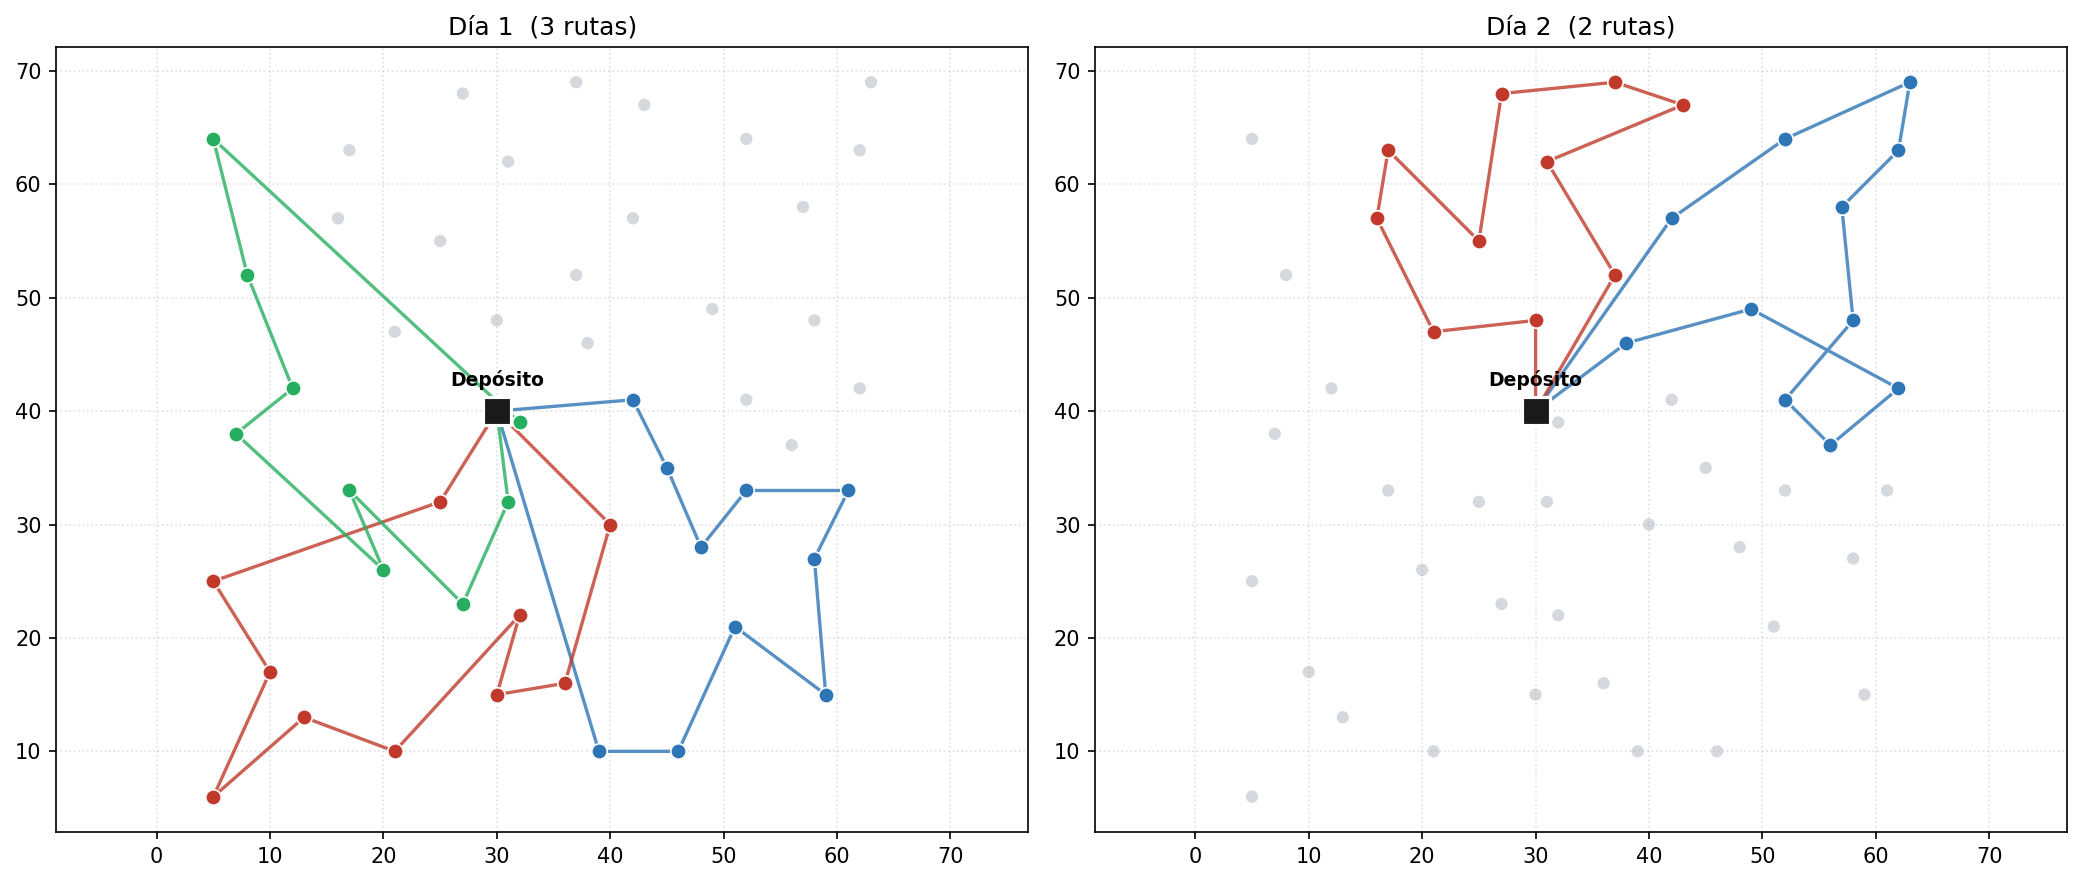
\includegraphics[width=\linewidth]{figures/rutas_p01_RL.png}
            \caption{Solución generada por el agente RL: Costo $617.4$, factible.}
        \end{subfigure}

        \begin{subfigure}{0.95\textwidth}
            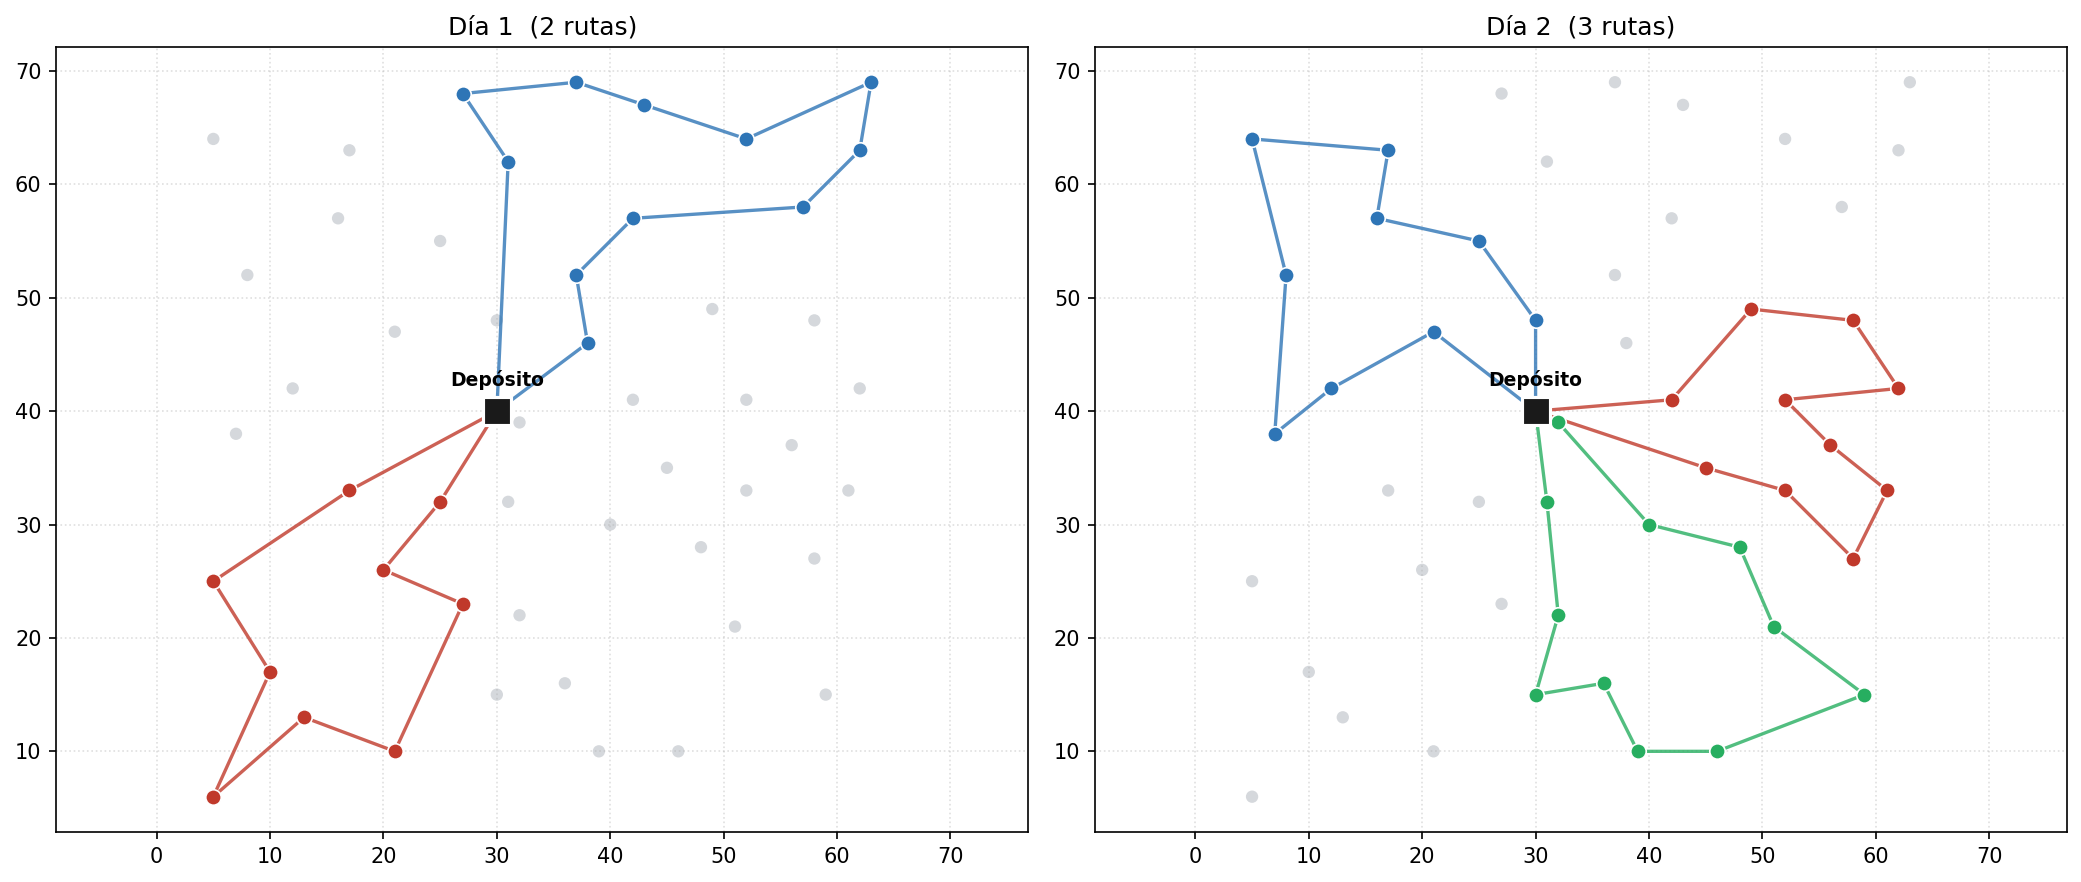
\includegraphics[width=\linewidth]{figures/rutas_p01_BKS.png}
            \caption{Mejor solución conocida BKS: Costo $524.6$.}
        \end{subfigure}
    \end{minipage}
    \caption{Rutas en la instancia $p01$.}
    \caption*{Fuente: Elaboración propia.}
    \label{fig:rutas-p01}
\end{figure}

Ambas soluciones logran agrupar a los clientes en zonas lógicas, pero la ruta del agente muestra algunos cruces de aristas que la mejor solución conocida logra evitar. Esto explica visualmente por qué existe ese gap. Tal como evidencia la figura, el agente es capaz de aprender la estructura global del problema, sabe qué clientes asignar a cada día y cómo agruparlos por vehículo, pero al construir la ruta paso a paso de forma secuencial, inevitablemente deja pequeños cruces que una heurística de mejora local sí limpiaría. Este patrón refleja una limitación inherente al enfoque constructivo puro y motiva las líneas de trabajo futuro.

\javi{Profe, respondo: (1) p01 es el caso principal porque fue la instancia sobre la que desarrollé y calibré el modelo, por su escala reducida y estructura simple. (2) El tiempo es de inferencia (agente ya entrenado construyendo la solución), no de entrenamiento. (3) La figura muestra una solución representativa del agente (costo 617,4), no la mejor; aclaré que está dentro del rango multi-semilla para que no se lea como cherry-picking. (4) Ya removí los títulos y ejes de los gráficos.}

%=============================================================%
\subsection{Resultados del escalamiento a $75$ y $100$ clientes} \label{sec:resultadosescalamiento}
%=============================================================%
Para evaluar si el método escala estructuralmente a instancias mayores, el agente se enfrentó a instancias de $75$ clientes ($p04$ de la familia A y $p06$ de la familia C) y de $100$ clientes ($p07$ de la familia A y $p09$ de la familia C), utilizando la configuración de red ampliada ($[512,512]$, $500\,000$ pasos). La Tabla~\ref{tab:escalamiento} consolida estos resultados, incluyendo también las instancias base de $50$ clientes ($p01$ y $p03$) para dimensionar el impacto del escalamiento. Esta tabla se centra deliberadamente en el contraste entre el agente RL y el VNS, su rival principal; los datos completos de la heurística Greedy, los costos absolutos, el BKS y los tiempos de ejecución para todas las instancias se reportan de forma integral en las Tablas~\ref{tab:consolidada} y~\ref{tab:tiempos} de la Sección~\ref{sec:comparacion-global}. \eli{¿no hay Greedy ni BKS ni tiempos?} \javi{Profe, esta tabla la dejé enfocada en RL vs VNS a propósito, para mostrar la degradación al escalar sin saturarla. Greedy, BKS y tiempos están completos en las tablas consolidadas de la Sección de comparación global (Tablas~\ref{tab:consolidada} y~\ref{tab:tiempos}).}

\begin{table}[H]
    \centering
    \caption{\label{tab:escalamiento} Resultados del escalamiento del agente a instancias de $75$ y $100$ clientes. Gap reportado como media $\pm$ desviación estándar sobre semillas factibles.}
    \caption*{Fuente: Elaboración propia.}
    \small
    \renewcommand{\arraystretch}{1.15}
    \setlength{\tabcolsep}{7pt}
    \begin{tabular}{@{}cccccc@{}}
        \toprule
        \textbf{Familia} & \textbf{Instancia} & \textbf{Clientes} & \textbf{Gap RL (\%)} & \textbf{Factibilidad} & \textbf{Gap VNS (\%)} \\
        \midrule
        \multirow{3}{*}{A} & $p01$ &  $50$ & $+19{,}7 \pm 6{,}5$ & $5/5$ & $+31{,}7$ \\
                           & $p04$ &  $75$ & $+53{,}9 \pm 5{,}4$ & $5/5$ & $+23{,}1$ \\
                           & $p07$ & $100$ & $+57{,}4 \pm 6{,}5$ & $5/5$ & $+27{,}3$ \\
        \midrule
        \multirow{3}{*}{C} & $p03$ &  $50$ & $+28{,}0 \pm 5{,}3$ & $5/5$ & $+83{,}8$ \\
                           & $p06$ &  $75$ & $+55{,}7 \pm 2{,}4$ & $4/5$ & $+104{,}7$ \\
                           & $p09$ & $100$ & $+66{,}7 \pm 5{,}7$ & $5/5$ & $+128{,}5$ \\
        \bottomrule
    \end{tabular}
\end{table}

El análisis de estos datos arroja tres observaciones clave. Primero, la factibilidad se mantiene en niveles sumamente altos en todas las escalas ($29$ de $30$ corridas factibles, logrando una tasa global del $97\%$), incluso al duplicar el número de clientes y aumentar el horizonte de planificación. Segundo, aunque la calidad respecto al BKS disminuye al crecer la instancia, esta degradación resulta suave y predecible: el mayor salto ocurre al pasar de $50$ a $75$ clientes, mientras que entre $75$ y $100$ el gap tiende a estabilizarse. Tercero, la pérdida de calidad es muy similar entre las familias A y C a igual escala, lo que demuestra que el rendimiento del modelo depende mucho más del tamaño del estado que de las restricciones temporales específicas de cada familia.

La Figura~\ref{fig:evolucion-gap} ilustra este patrón. El gráfico muestra la evolución del gap medio respecto al BKS en función del número de clientes, tanto para el agente RL (familias A y C) como para VNS (familia A). Aquí queda en evidencia que el agente RL experimenta un salto pronunciado en el gap entre $50$ y $75$ clientes, seguido de una estabilización hacia los $100$. En contraste, la heurística VNS logra mantener gaps casi constantes en la familia A a lo largo de las tres escalas.

\begin{figure}[H]
    \centering
    \begin{tikzpicture}
        \begin{axis}[
            width=10cm,
            height=6.6cm,
            xlabel={Número de clientes},
            ylabel={Gap medio respecto al BKS (\%)},
            xmin=45, xmax=105,
            ymin=0, ymax=75,
            xtick={50,75,100},
            ytick={0,10,20,30,40,50,60,70},
            grid=major,
            xmajorgrids=true,
            ymajorgrids=true,
            grid style={line width=0.3pt, draw=gray!30},
            axis line style={black!70},
            tick style={black!70},
            tick label style={font=\small},
            label style={font=\small},
            legend style={
                font=\small,
                draw=black!40,
                fill=white,
                rounded corners=2pt,
                at={(1.04,0.5)},
                anchor=west
            },
            legend cell align=left,
            clip=false
        ]
            \addplot[color=blue!70!black, thick, mark=*, mark size=2.8pt]
            coordinates {(50,19.7) (75,53.9) (100,57.4)};
            \addlegendentry{RL familia A}

            \addplot[color=red!70!black, thick, mark=square*, mark size=2.8pt]
            coordinates {(50,28.0) (75,55.7) (100,66.7)};
            \addlegendentry{RL familia C}

            \addplot[color=gray!65, thick, dashed, mark=triangle*, mark size=3pt]
            coordinates {(50,31.7) (75,23.1) (100,27.3)};
            \addlegendentry{VNS familia A}
        \end{axis}
    \end{tikzpicture}
    \caption{Evolución del gap medio respecto al BKS según el número de clientes.}
    \caption*{Fuente: Elaboración propia.}
    \label{fig:evolucion-gap}
\end{figure}

Para complementar los números con evidencia visual, las Figuras~\ref{fig:rutas-p03} a~\ref{fig:rutas-p09-bks} contrastan soluciones representativas construidas por el agente con las mejores soluciones conocidas, organizadas según el tamaño de la instancia ($50$, $75$ y $100$ clientes) para observar directamente el efecto del escalamiento.

Comenzando con la escala base de $50$ clientes, la Figura~\ref{fig:rutas-p03} expone la instancia $p03$ (familia C, horizonte de 5 días, un vehículo). En este escenario, el agente logra un gap de $+28{,}0\%$, superando por un amplio margen el $+83{,}8\%$ de VNS. Visualmente, se aprecia que el modelo RL genera agrupaciones sumamente limpias, con muy pocos cruces locales.

\begin{figure}[H]
    \centering
    \begin{minipage}{0.95\textwidth}
        \centering
        \begin{subfigure}{0.95\textwidth}
            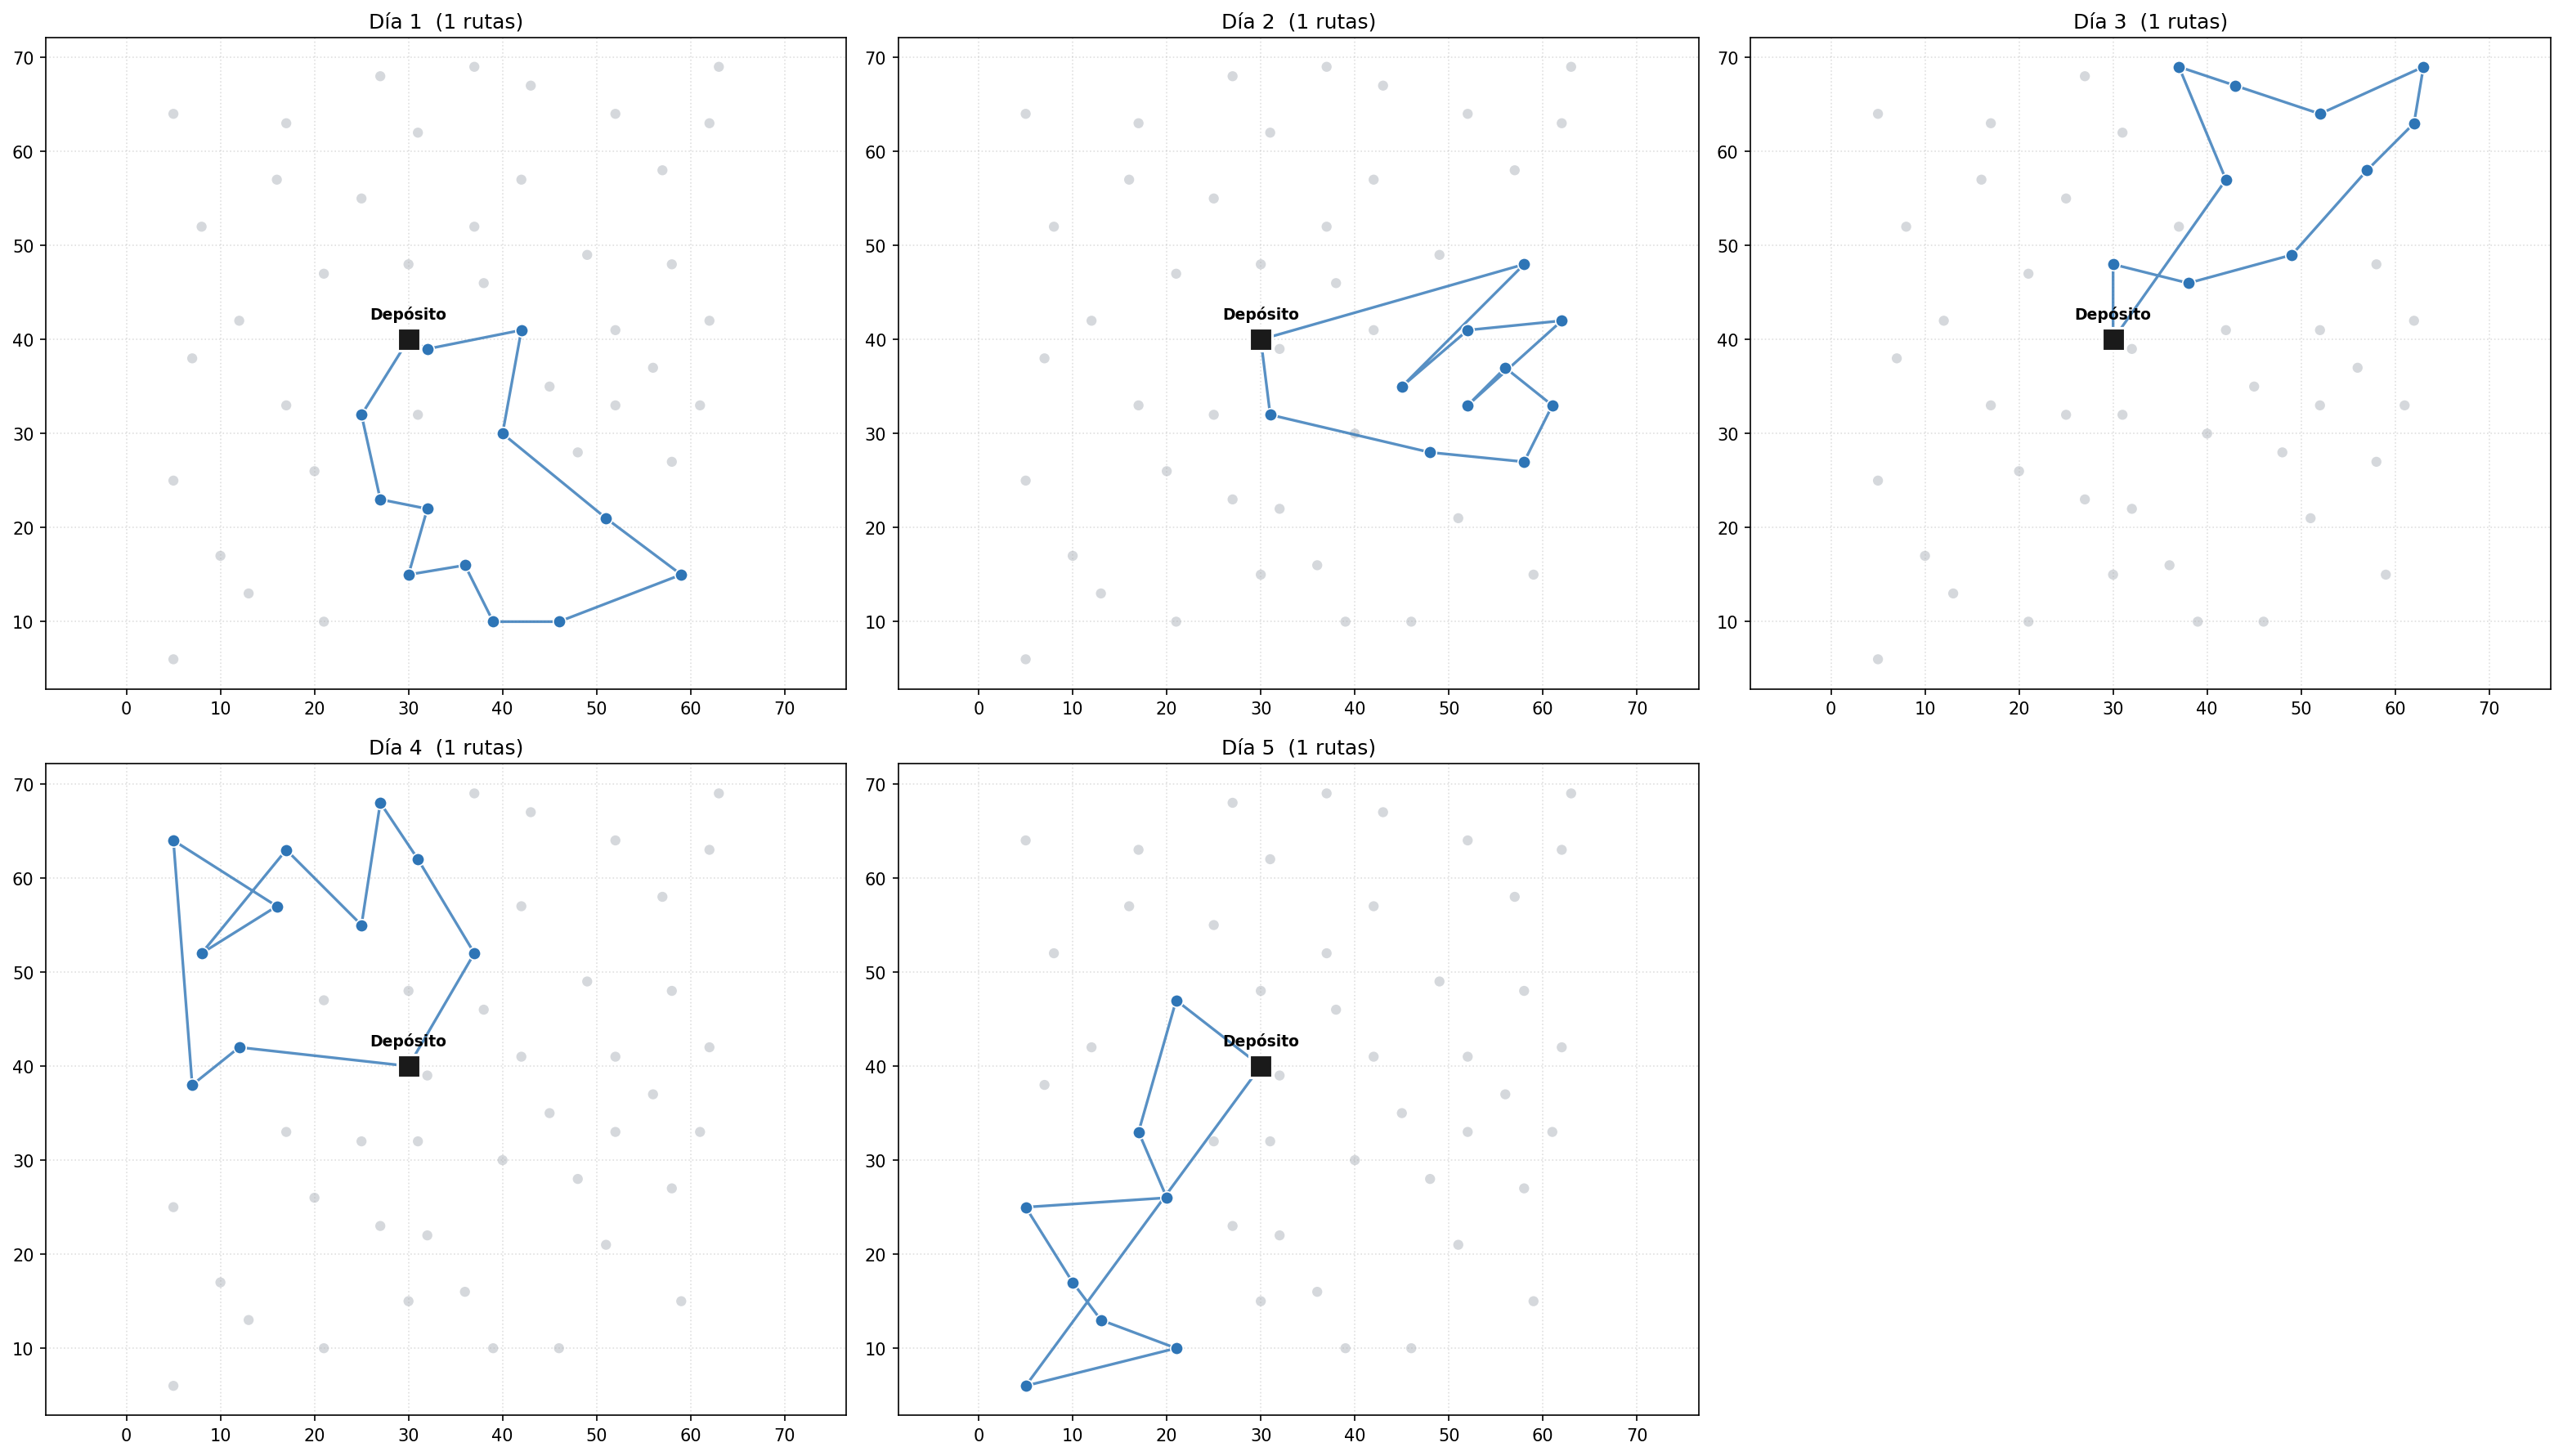
\includegraphics[width=\linewidth]{figures/rutas_p03_RL.png}
            \caption{Solución generada por el agente RL: Costo $636.5$, factible.}
        \end{subfigure}

        \begin{subfigure}{0.95\textwidth}
            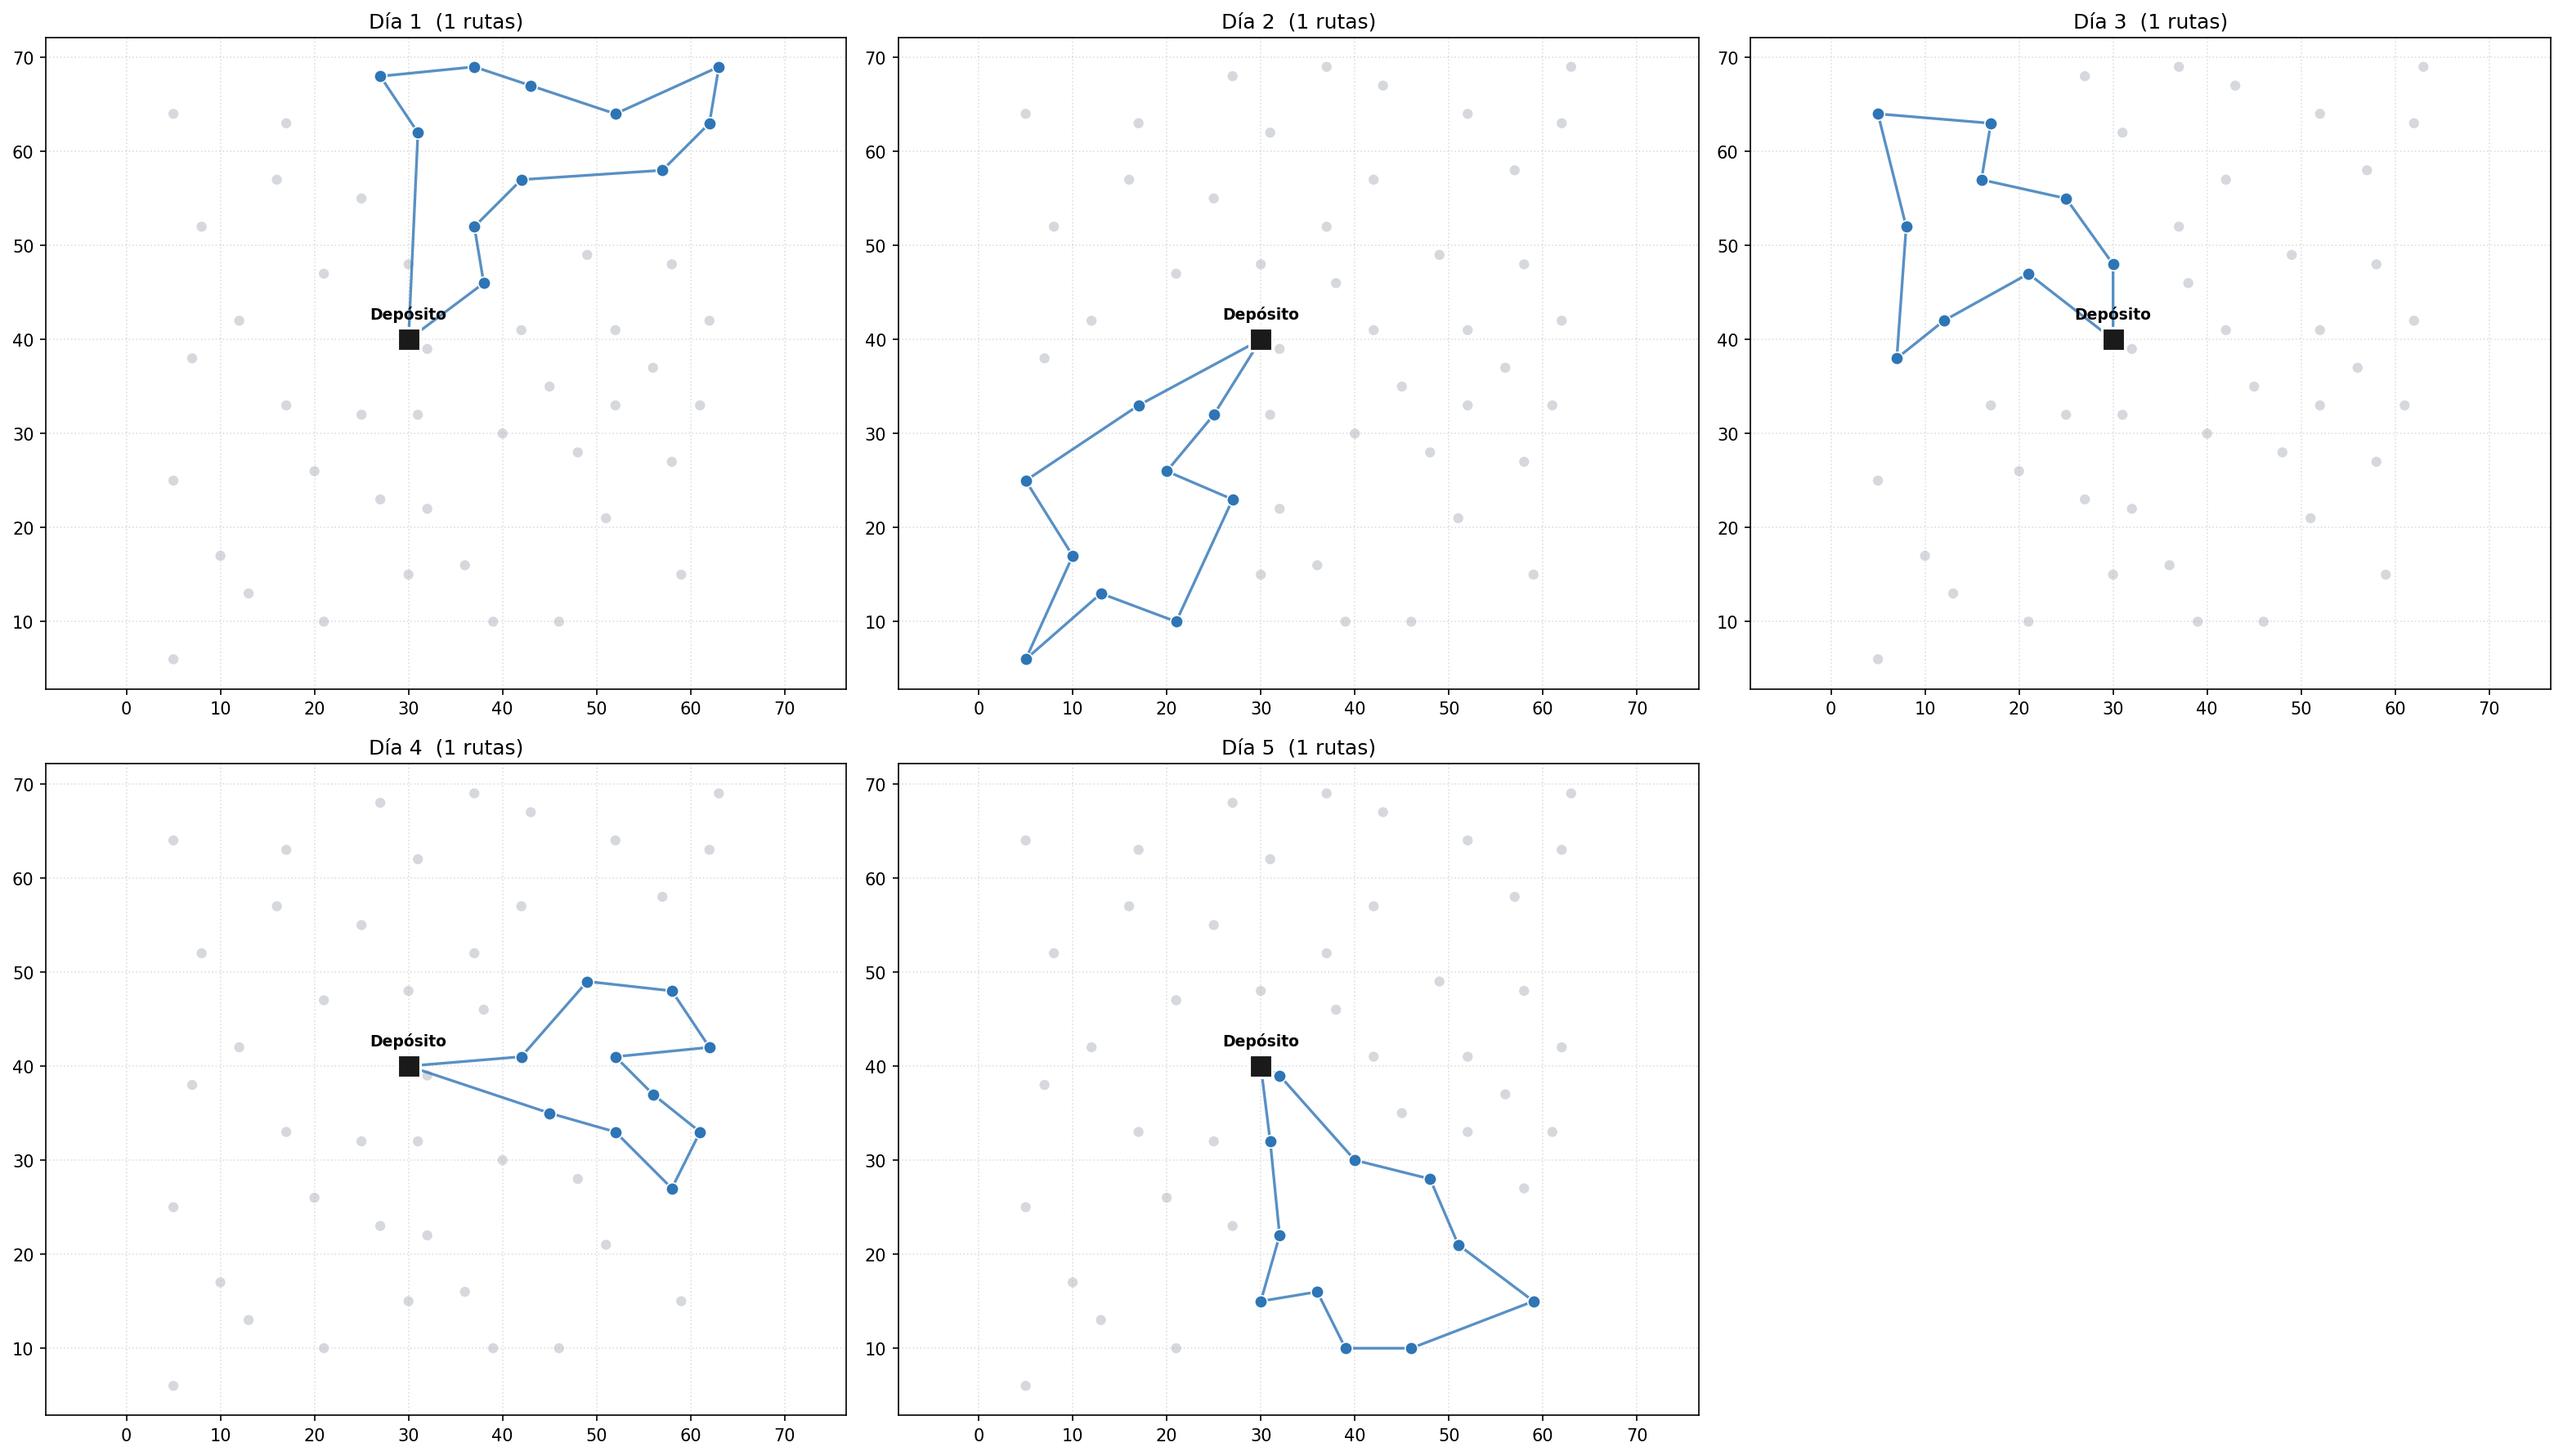
\includegraphics[width=\linewidth]{figures/rutas_p03_BKS.png}
            \caption{Mejor solución conocida BKS: Costo $524.6$.}
        \end{subfigure}
    \end{minipage}
    \caption{Rutas en la instancia $p03$.}
    \caption*{Fuente: Elaboración propia.}
    \label{fig:rutas-p03}
\end{figure}

Al subir a la escala de $75$ clientes, las Figuras~\ref{fig:rutas-p04} y~\ref{fig:rutas-p06-rl} muestran el comportamiento en las familias A y C, respectivamente. La Figura~\ref{fig:rutas-p04} presenta los resultados de la instancia $p04$ (familia A, horizonte de 2 días, cinco vehículos), donde la mayor densidad de puntos y la cantidad de vehículos por día introducen una complejidad combinatoria superior. Por su parte, las Figuras~\ref{fig:rutas-p06-rl} y~\ref{fig:rutas-p06-bks} ilustran los resultados de la instancia $p06$ (familia C, horizonte de 10 días, un vehículo), exigiendo al agente construir una secuencia temporal muy extensa. En ambos casos, el agente mantiene una zonificación global correcta, pero el aumento de puntos provoca que los cruces de aristas locales comiencen a acumularse.

\begin{figure}[H]
    \centering
    \begin{minipage}{0.95\textwidth}
        \centering
        \begin{subfigure}{0.95\textwidth}
            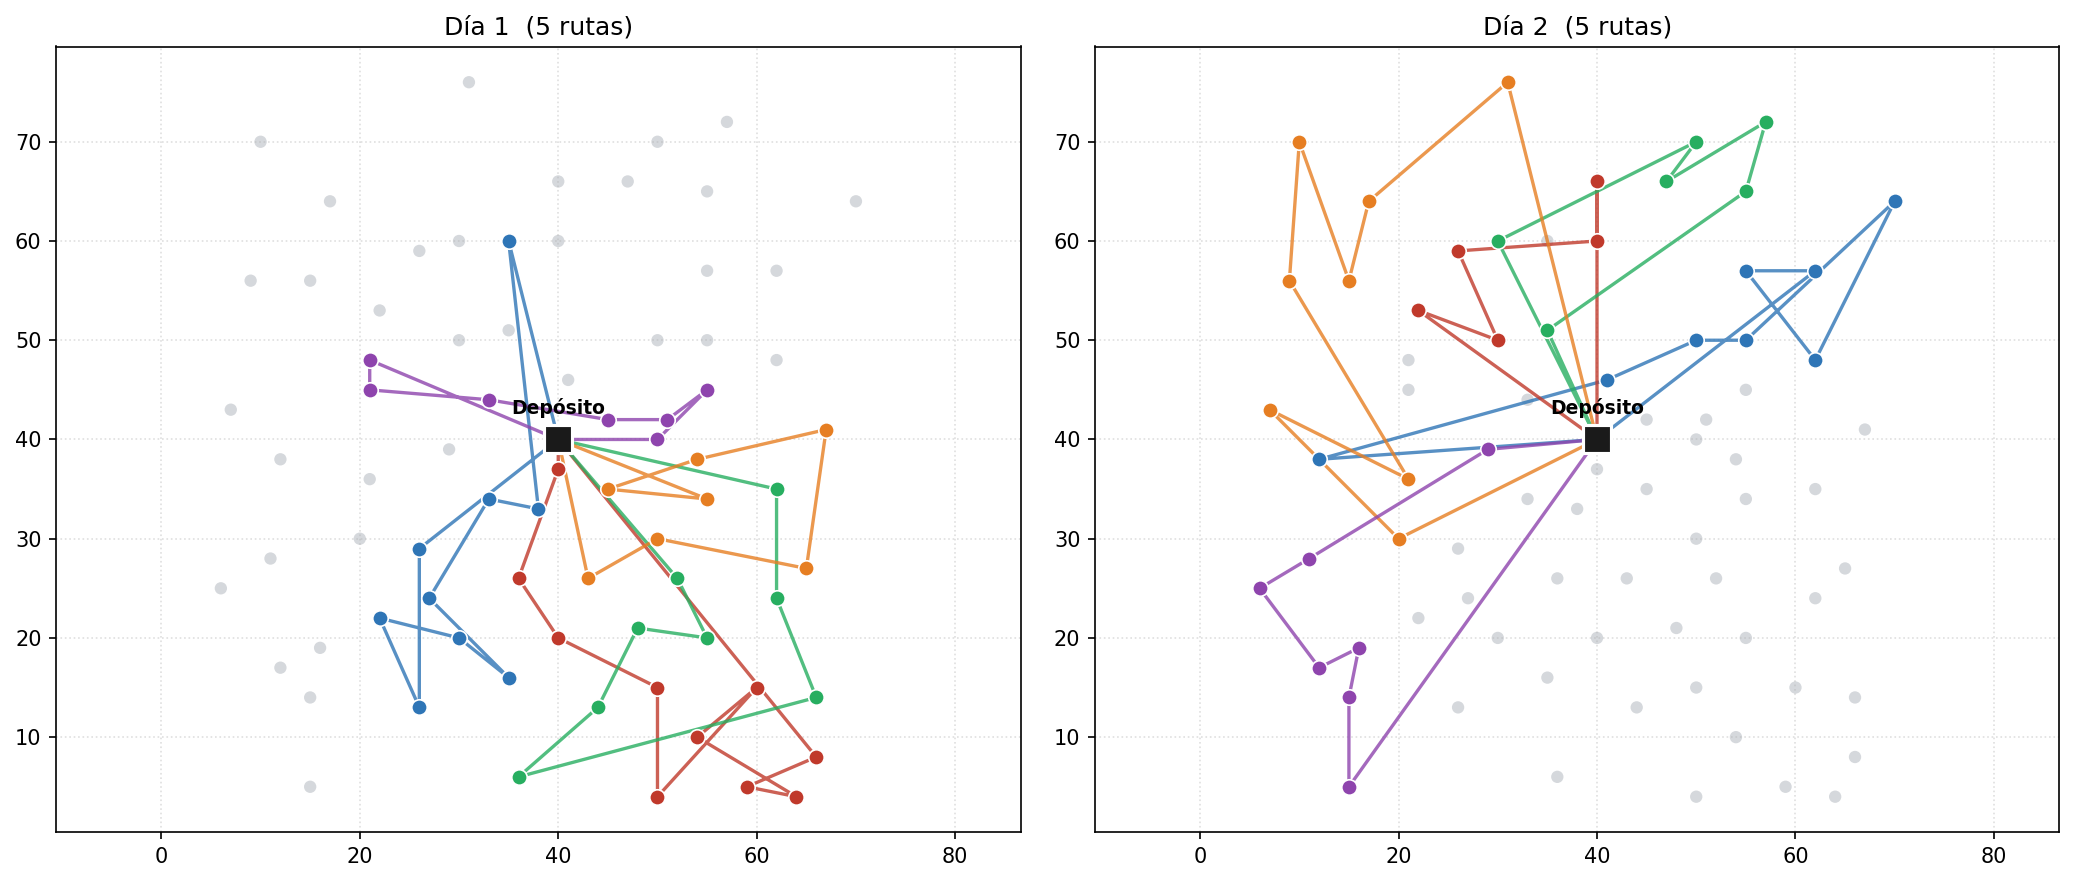
\includegraphics[width=\linewidth]{figures/rutas_p04_RL.png}
            \caption{Solución generada por el agente RL: Costo $1201.8$, factible.}
        \end{subfigure}

        \begin{subfigure}{0.95\textwidth}
            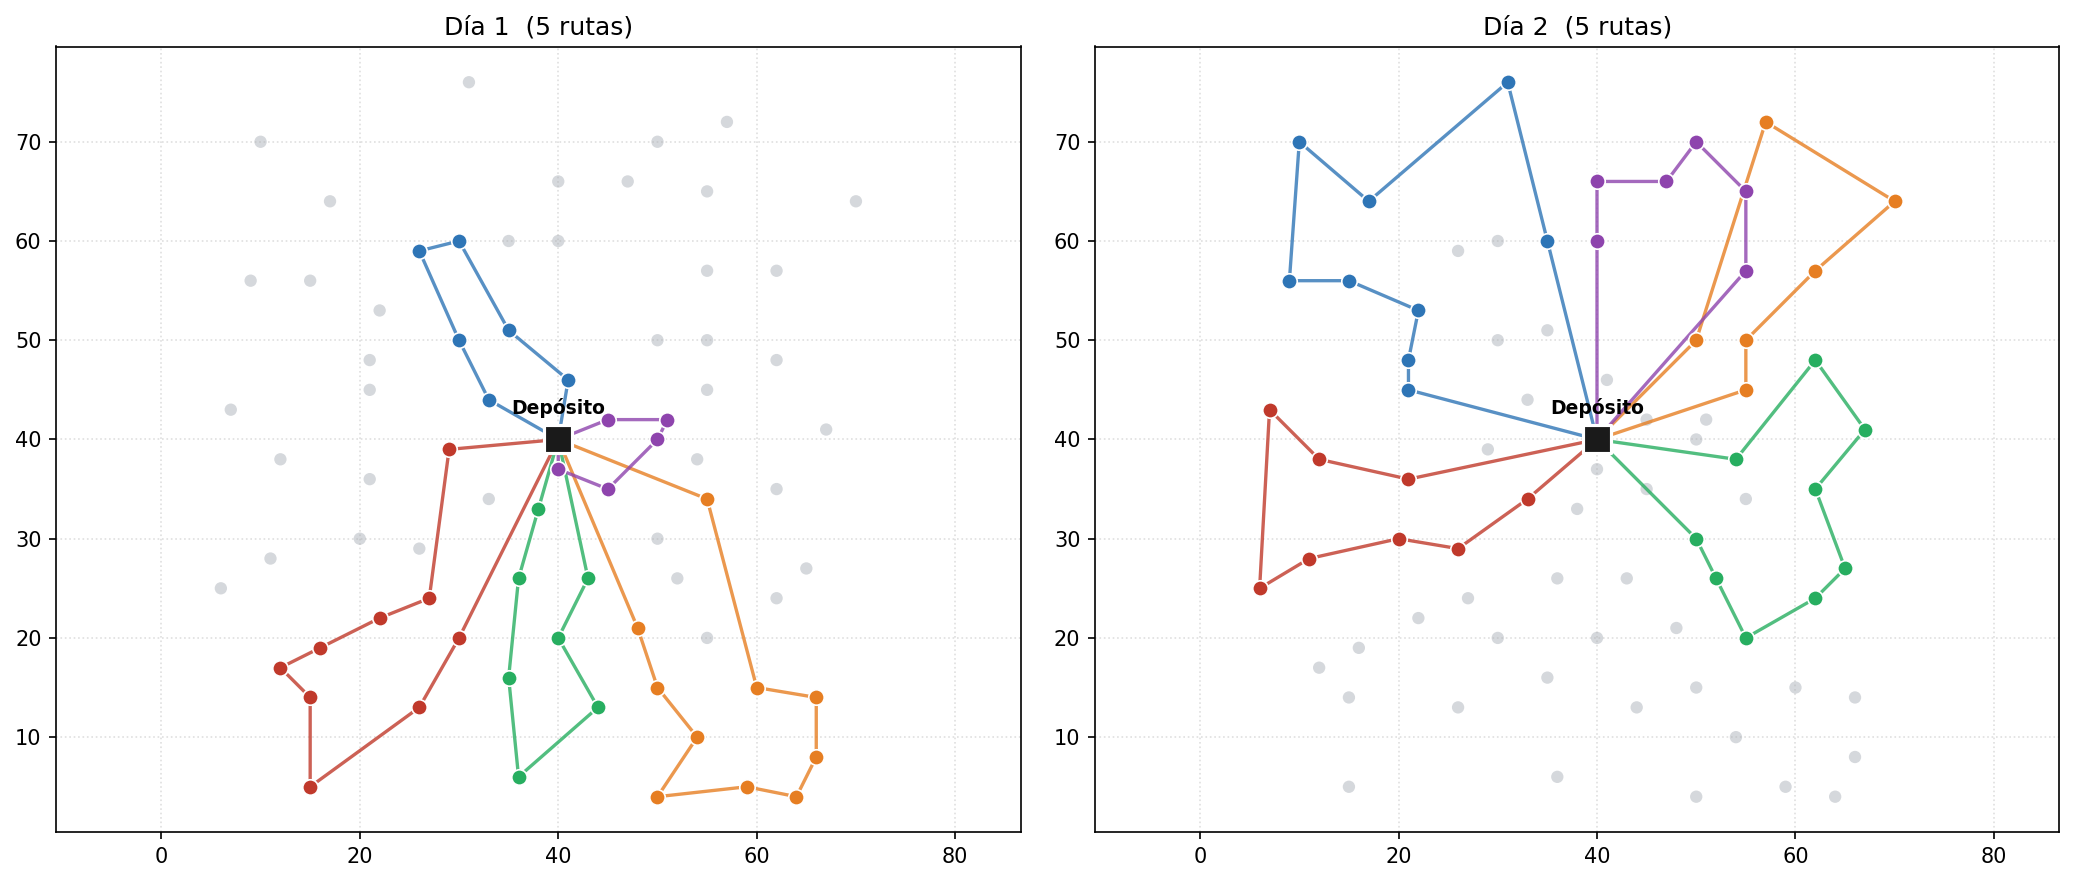
\includegraphics[width=\linewidth]{figures/rutas_p04_BKS.png}
            \caption{Mejor solución conocida BKS: Costo $835.4$.}
        \end{subfigure}
    \end{minipage}
    \caption{Rutas en la instancia $p04$.}
    \caption*{Fuente: Elaboración propia.}
    \label{fig:rutas-p04}
\end{figure}

\clearpage
\begin{figure}[H]
    \centering
    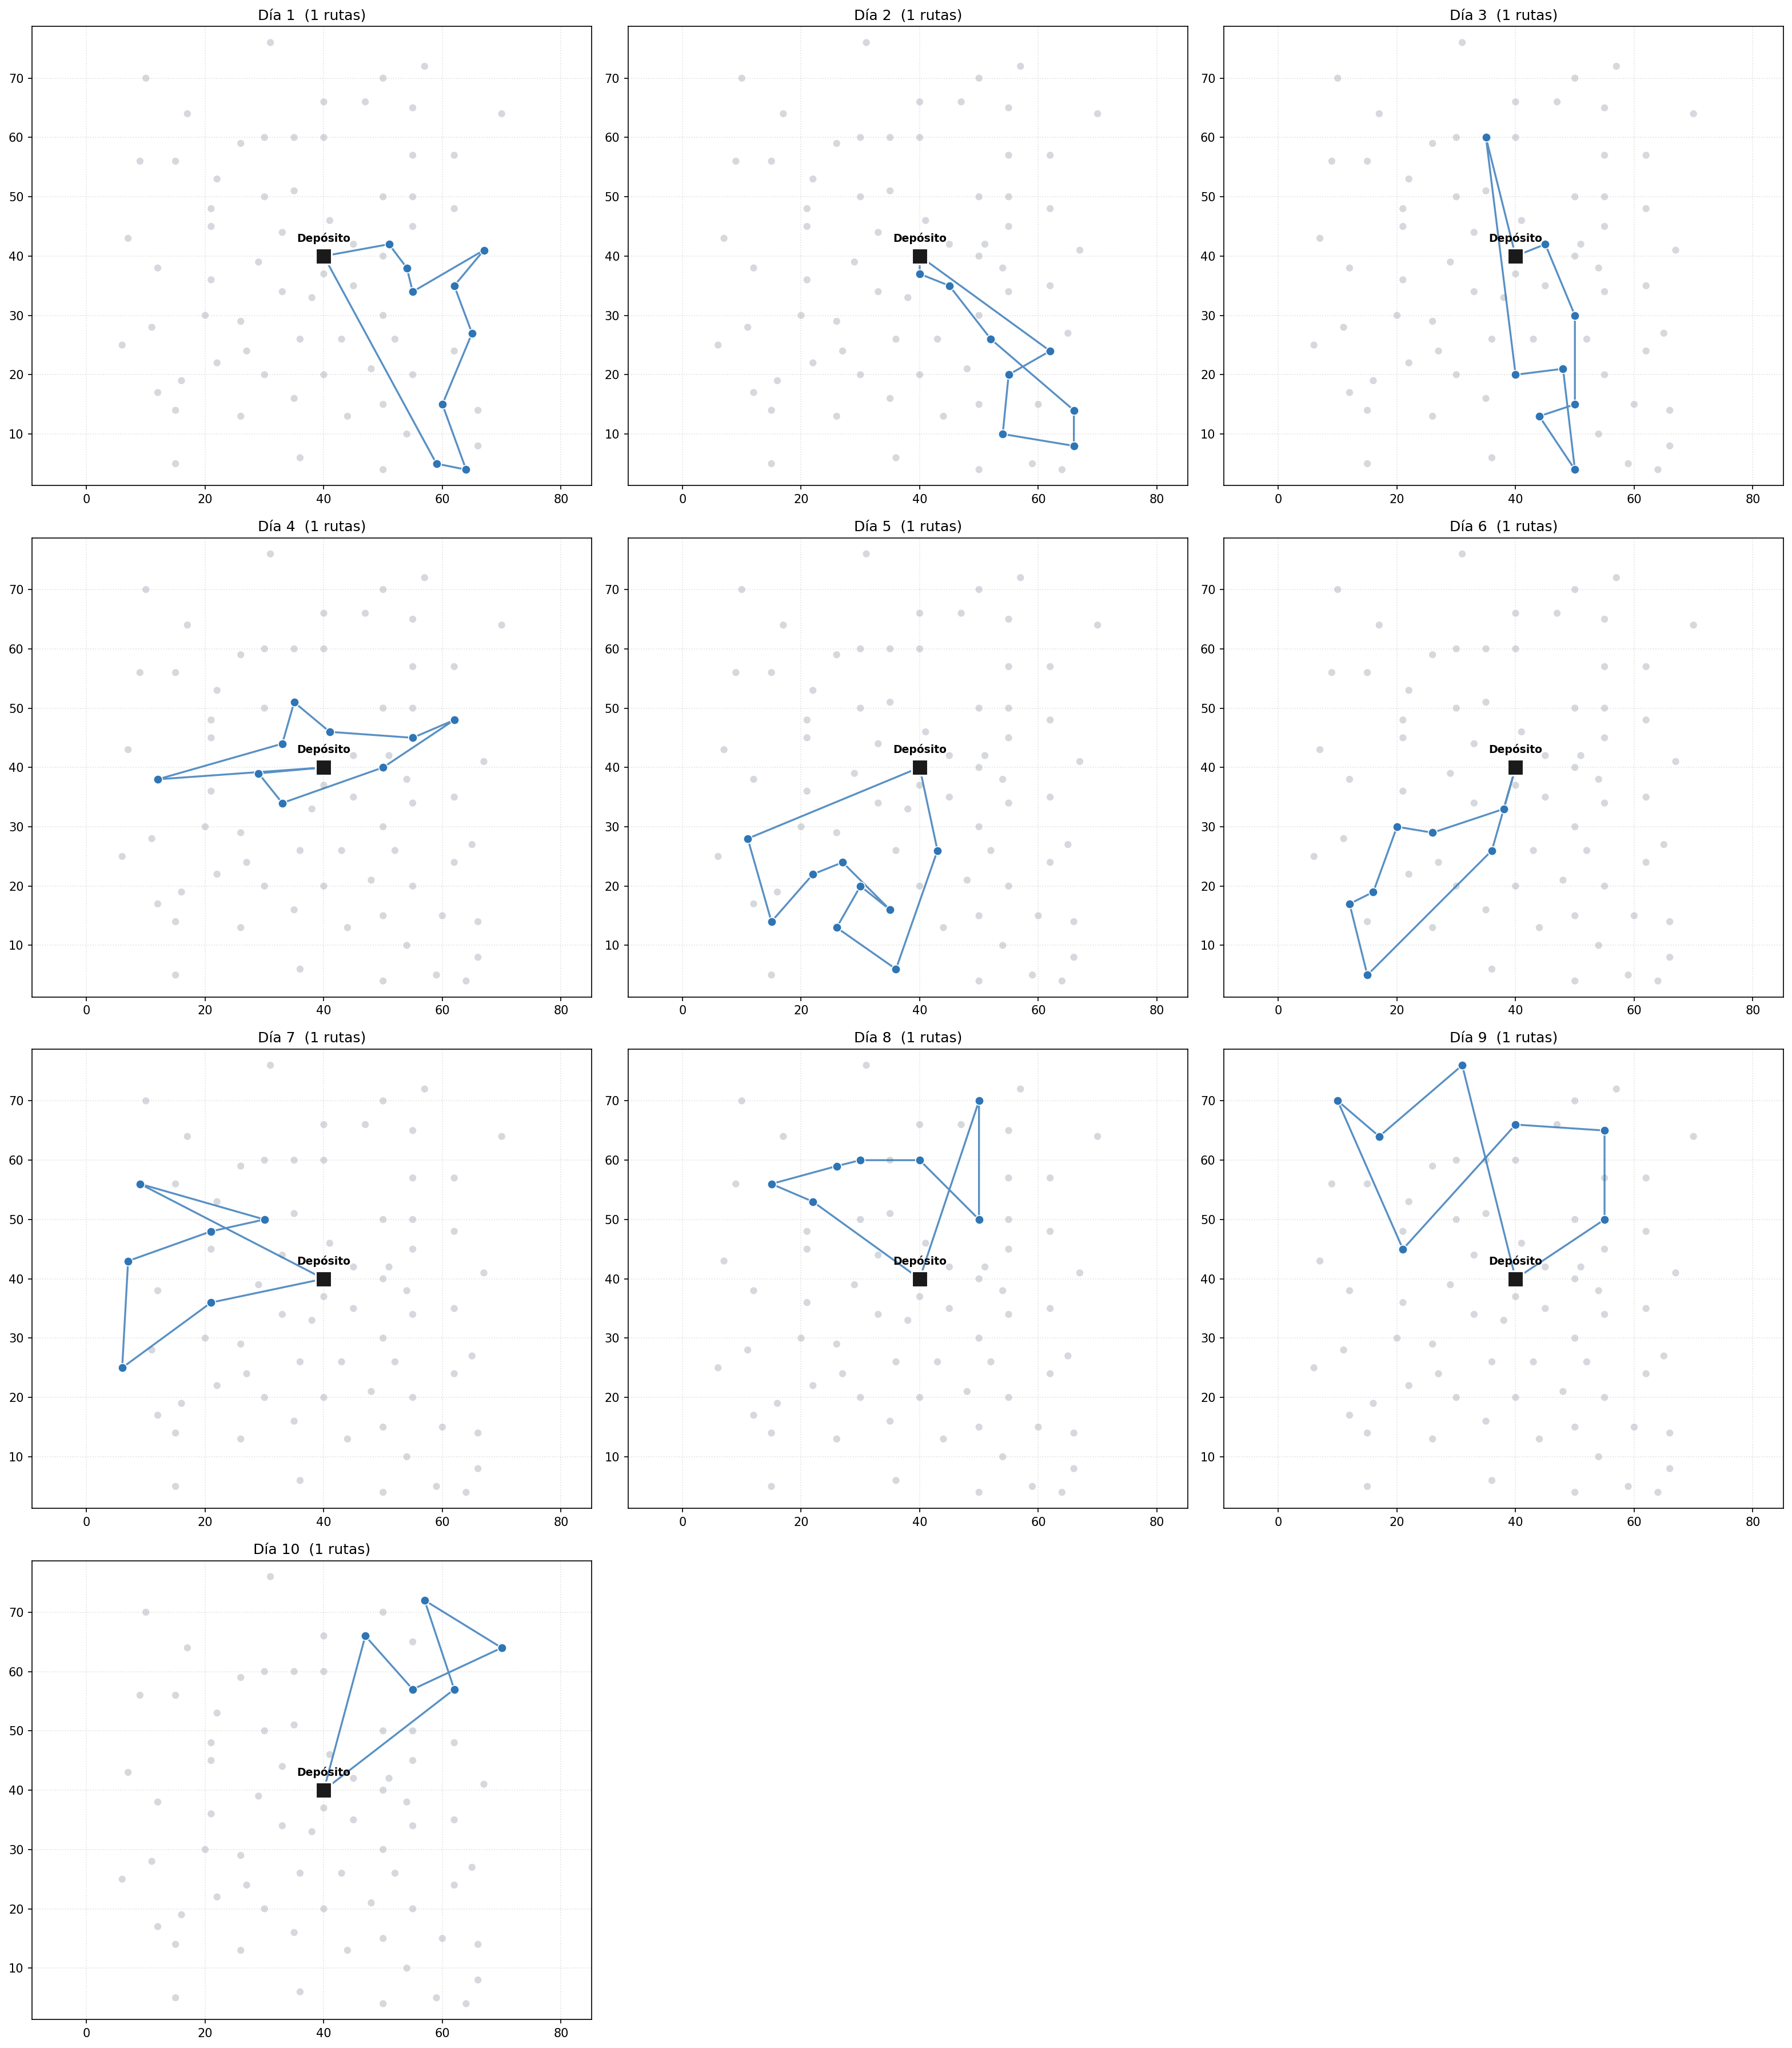
\includegraphics[
        width=\linewidth,
        height=0.80\textheight,
        keepaspectratio
    ]{figures/rutas_p06_RL.png}
    \caption{Rutas en la instancia $p06$ generadas por el agente RL: costo $1270{,}2$, factible.}
    \caption*{Fuente: Elaboración propia.}
    \label{fig:rutas-p06-rl}
\end{figure}

\clearpage
\begin{figure}[H]
    \centering
    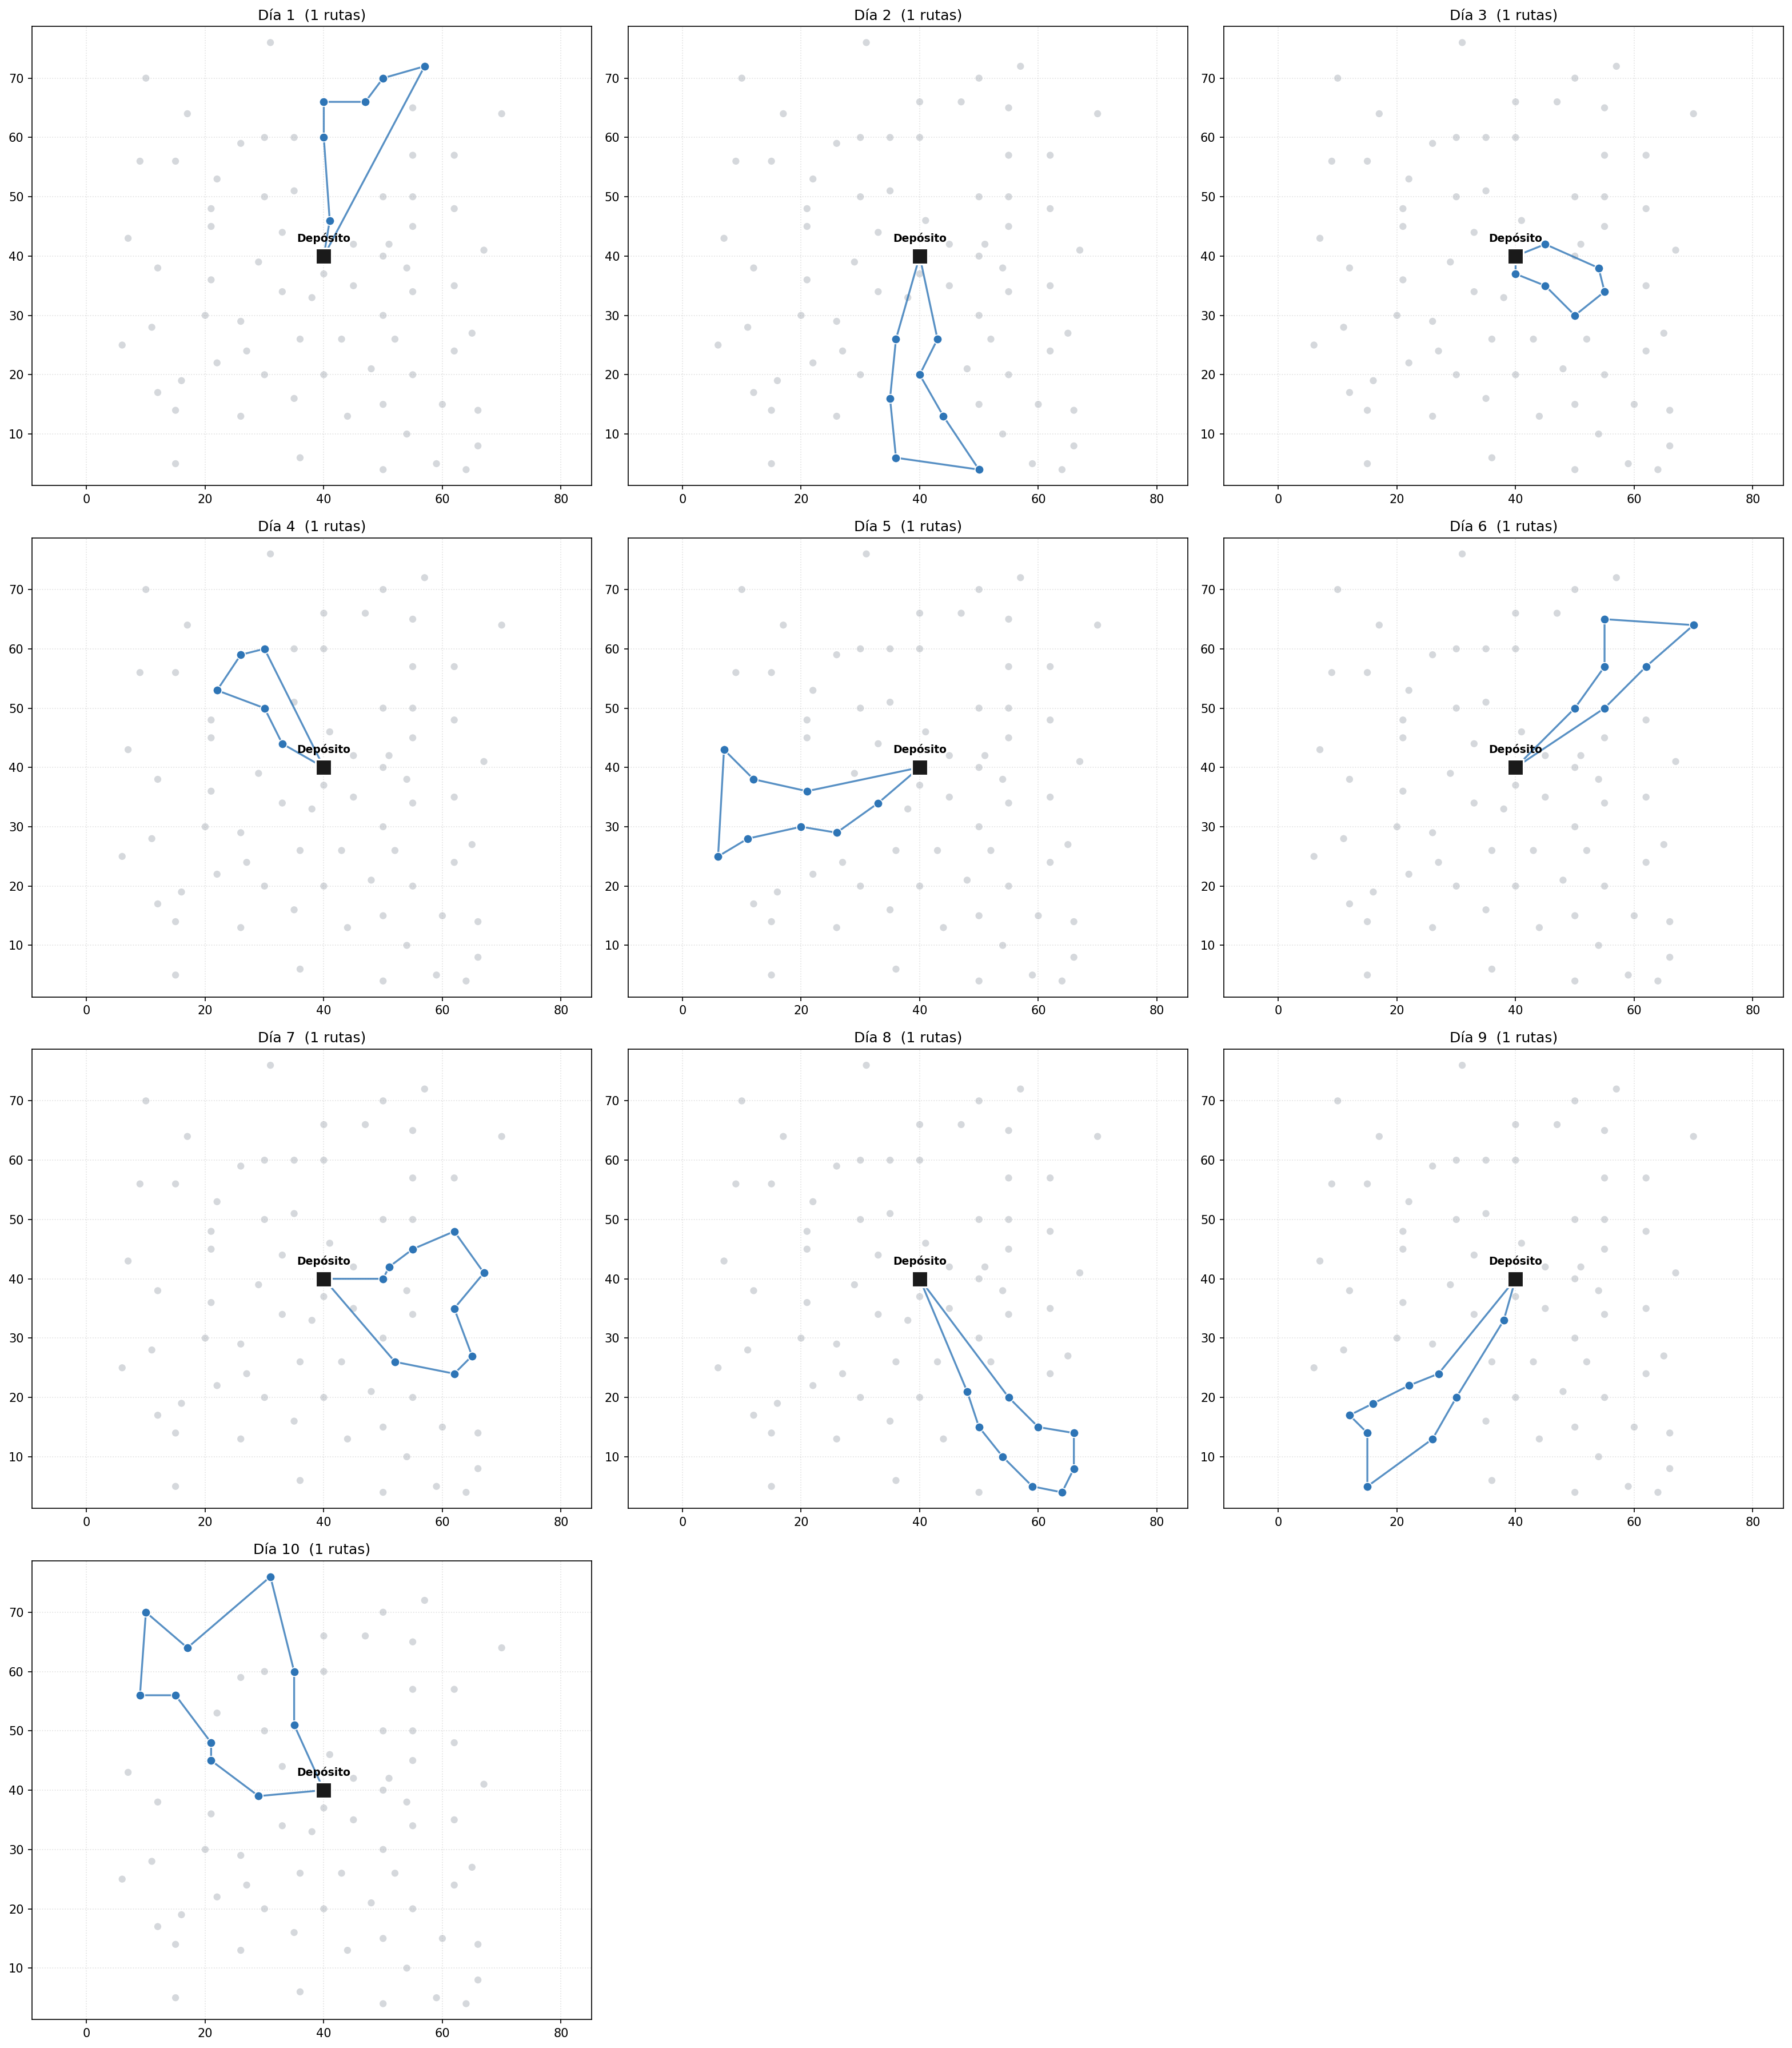
\includegraphics[
        width=\linewidth,
        height=0.80\textheight,
        keepaspectratio
    ]{figures/rutas_p06_BKS.png}
    \caption{Mejor solución conocida (BKS) para la instancia $p06$: costo $836{,}4$.}
    \caption*{Fuente: Elaboración propia.}
    \label{fig:rutas-p06-bks}
\end{figure}

Finalmente, al llegar a la escala máxima de $100$ clientes, las Figuras~\ref{fig:rutas-p07} y~\ref{fig:rutas-p09-rl} evidencian cómo el modelo maneja la mayor densidad geométrica posible del estudio. La Figura~\ref{fig:rutas-p07} presenta los resultados de la instancia $p07$ (familia A, horizonte de 2 días, cuatro vehículos), y las Figuras~\ref{fig:rutas-p09-rl} y~\ref{fig:rutas-p09-bks} presentan los resultados de la instancia $p09$ (familia C, horizonte de 8 días, un vehículo). A pesar de enfrentar la escala más exigente, el agente conserva su capacidad de generar soluciones factibles y reparte la demanda de forma coherente. Sin embargo, la falta de refinamiento local en un enfoque puramente constructivo se hace evidente: la densidad extrema de clientes multiplica las decisiones subóptimas a nivel de nodo, consolidando el gap documentado.

\begin{figure}[H]
    \centering
    \begin{minipage}{0.95\textwidth}
        \centering
        \begin{subfigure}{0.95\textwidth}
            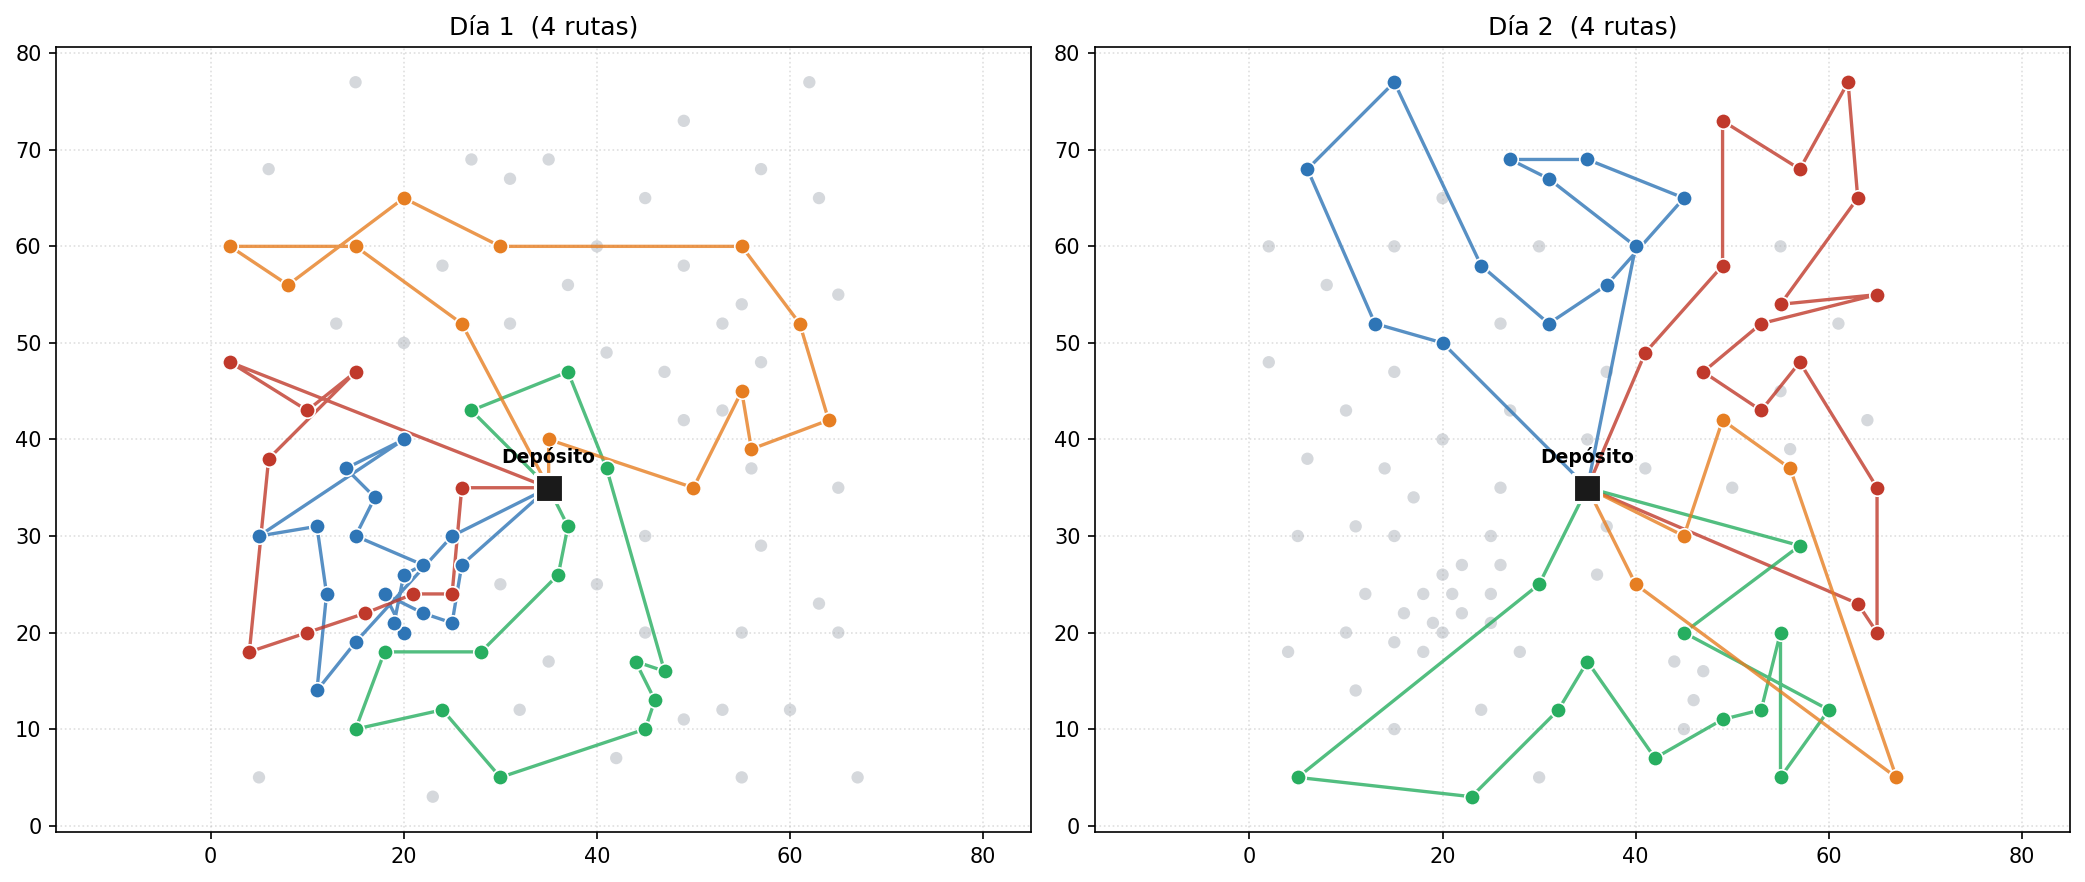
\includegraphics[width=\linewidth]{figures/rutas_p07_RL.png}
            \caption{Solución generada por el agente RL: Costo $1238.5$, factible.}
        \end{subfigure}

        \begin{subfigure}{0.95\textwidth}
            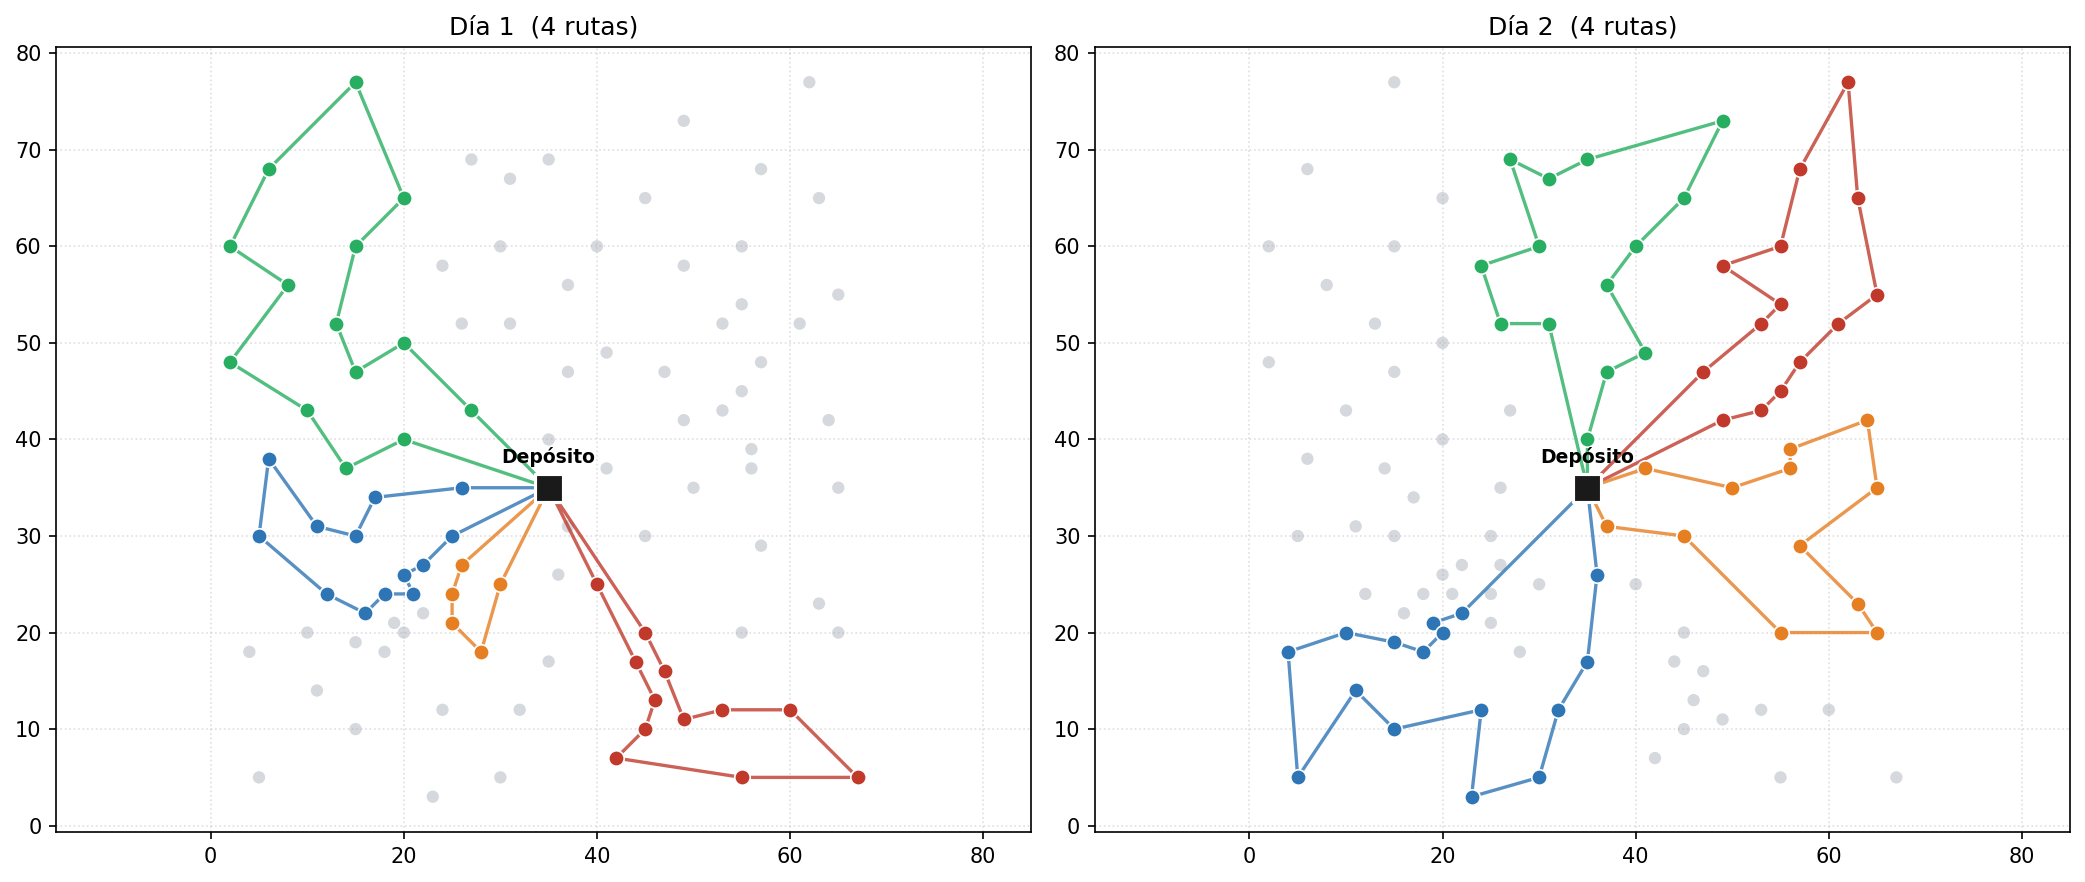
\includegraphics[width=\linewidth]{figures/rutas_p07_BKS.png}
            \caption{Mejor solución conocida BKS: Costo $826.1$.}
        \end{subfigure}
    \end{minipage}
    \caption{Rutas en la instancia $p07$.}
    \caption*{Fuente: Elaboración propia.}
    \label{fig:rutas-p07}
\end{figure}

\clearpage
\begin{figure}[H]
    \centering
    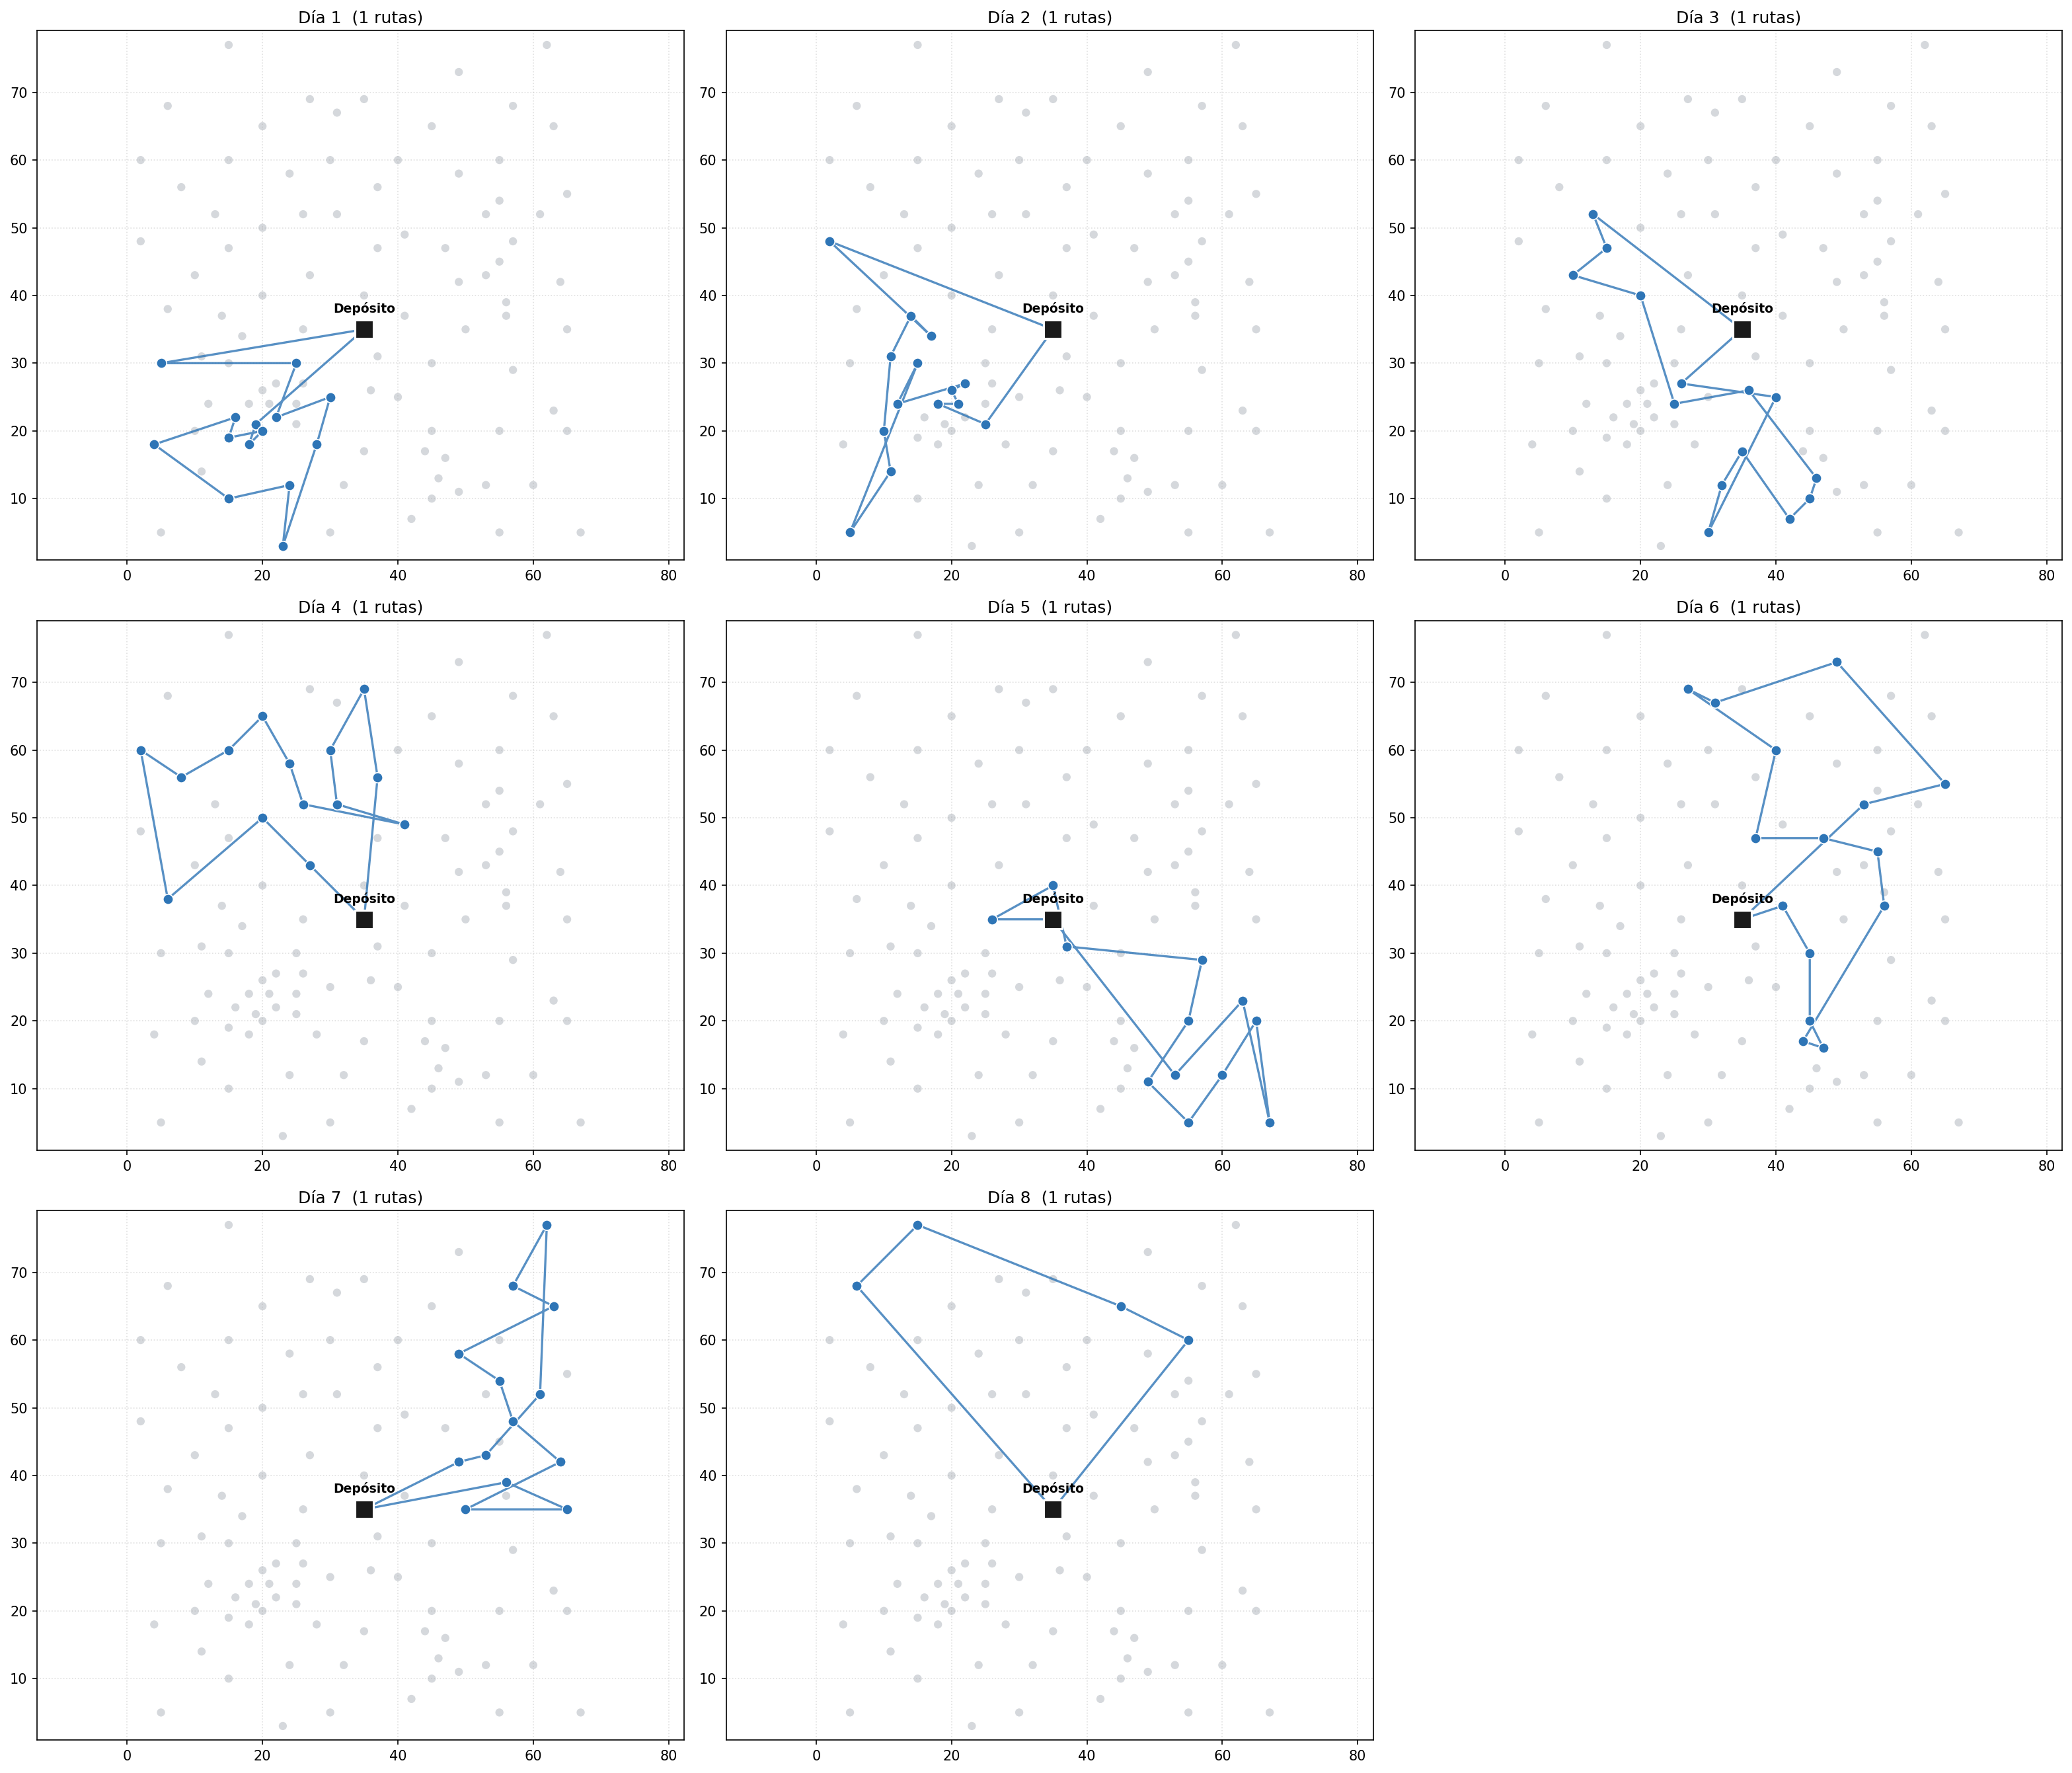
\includegraphics[
        width=\linewidth,
        height=0.80\textheight,
        keepaspectratio
    ]{figures/rutas_p09_RL.png}
    \caption{Rutas en la instancia $p09$ generadas por el agente RL: costo $1369{,}2$, factible.}
    \caption*{Fuente: Elaboración propia.}
    \label{fig:rutas-p09-rl}
\end{figure}

\clearpage
\begin{figure}[H]
    \centering
    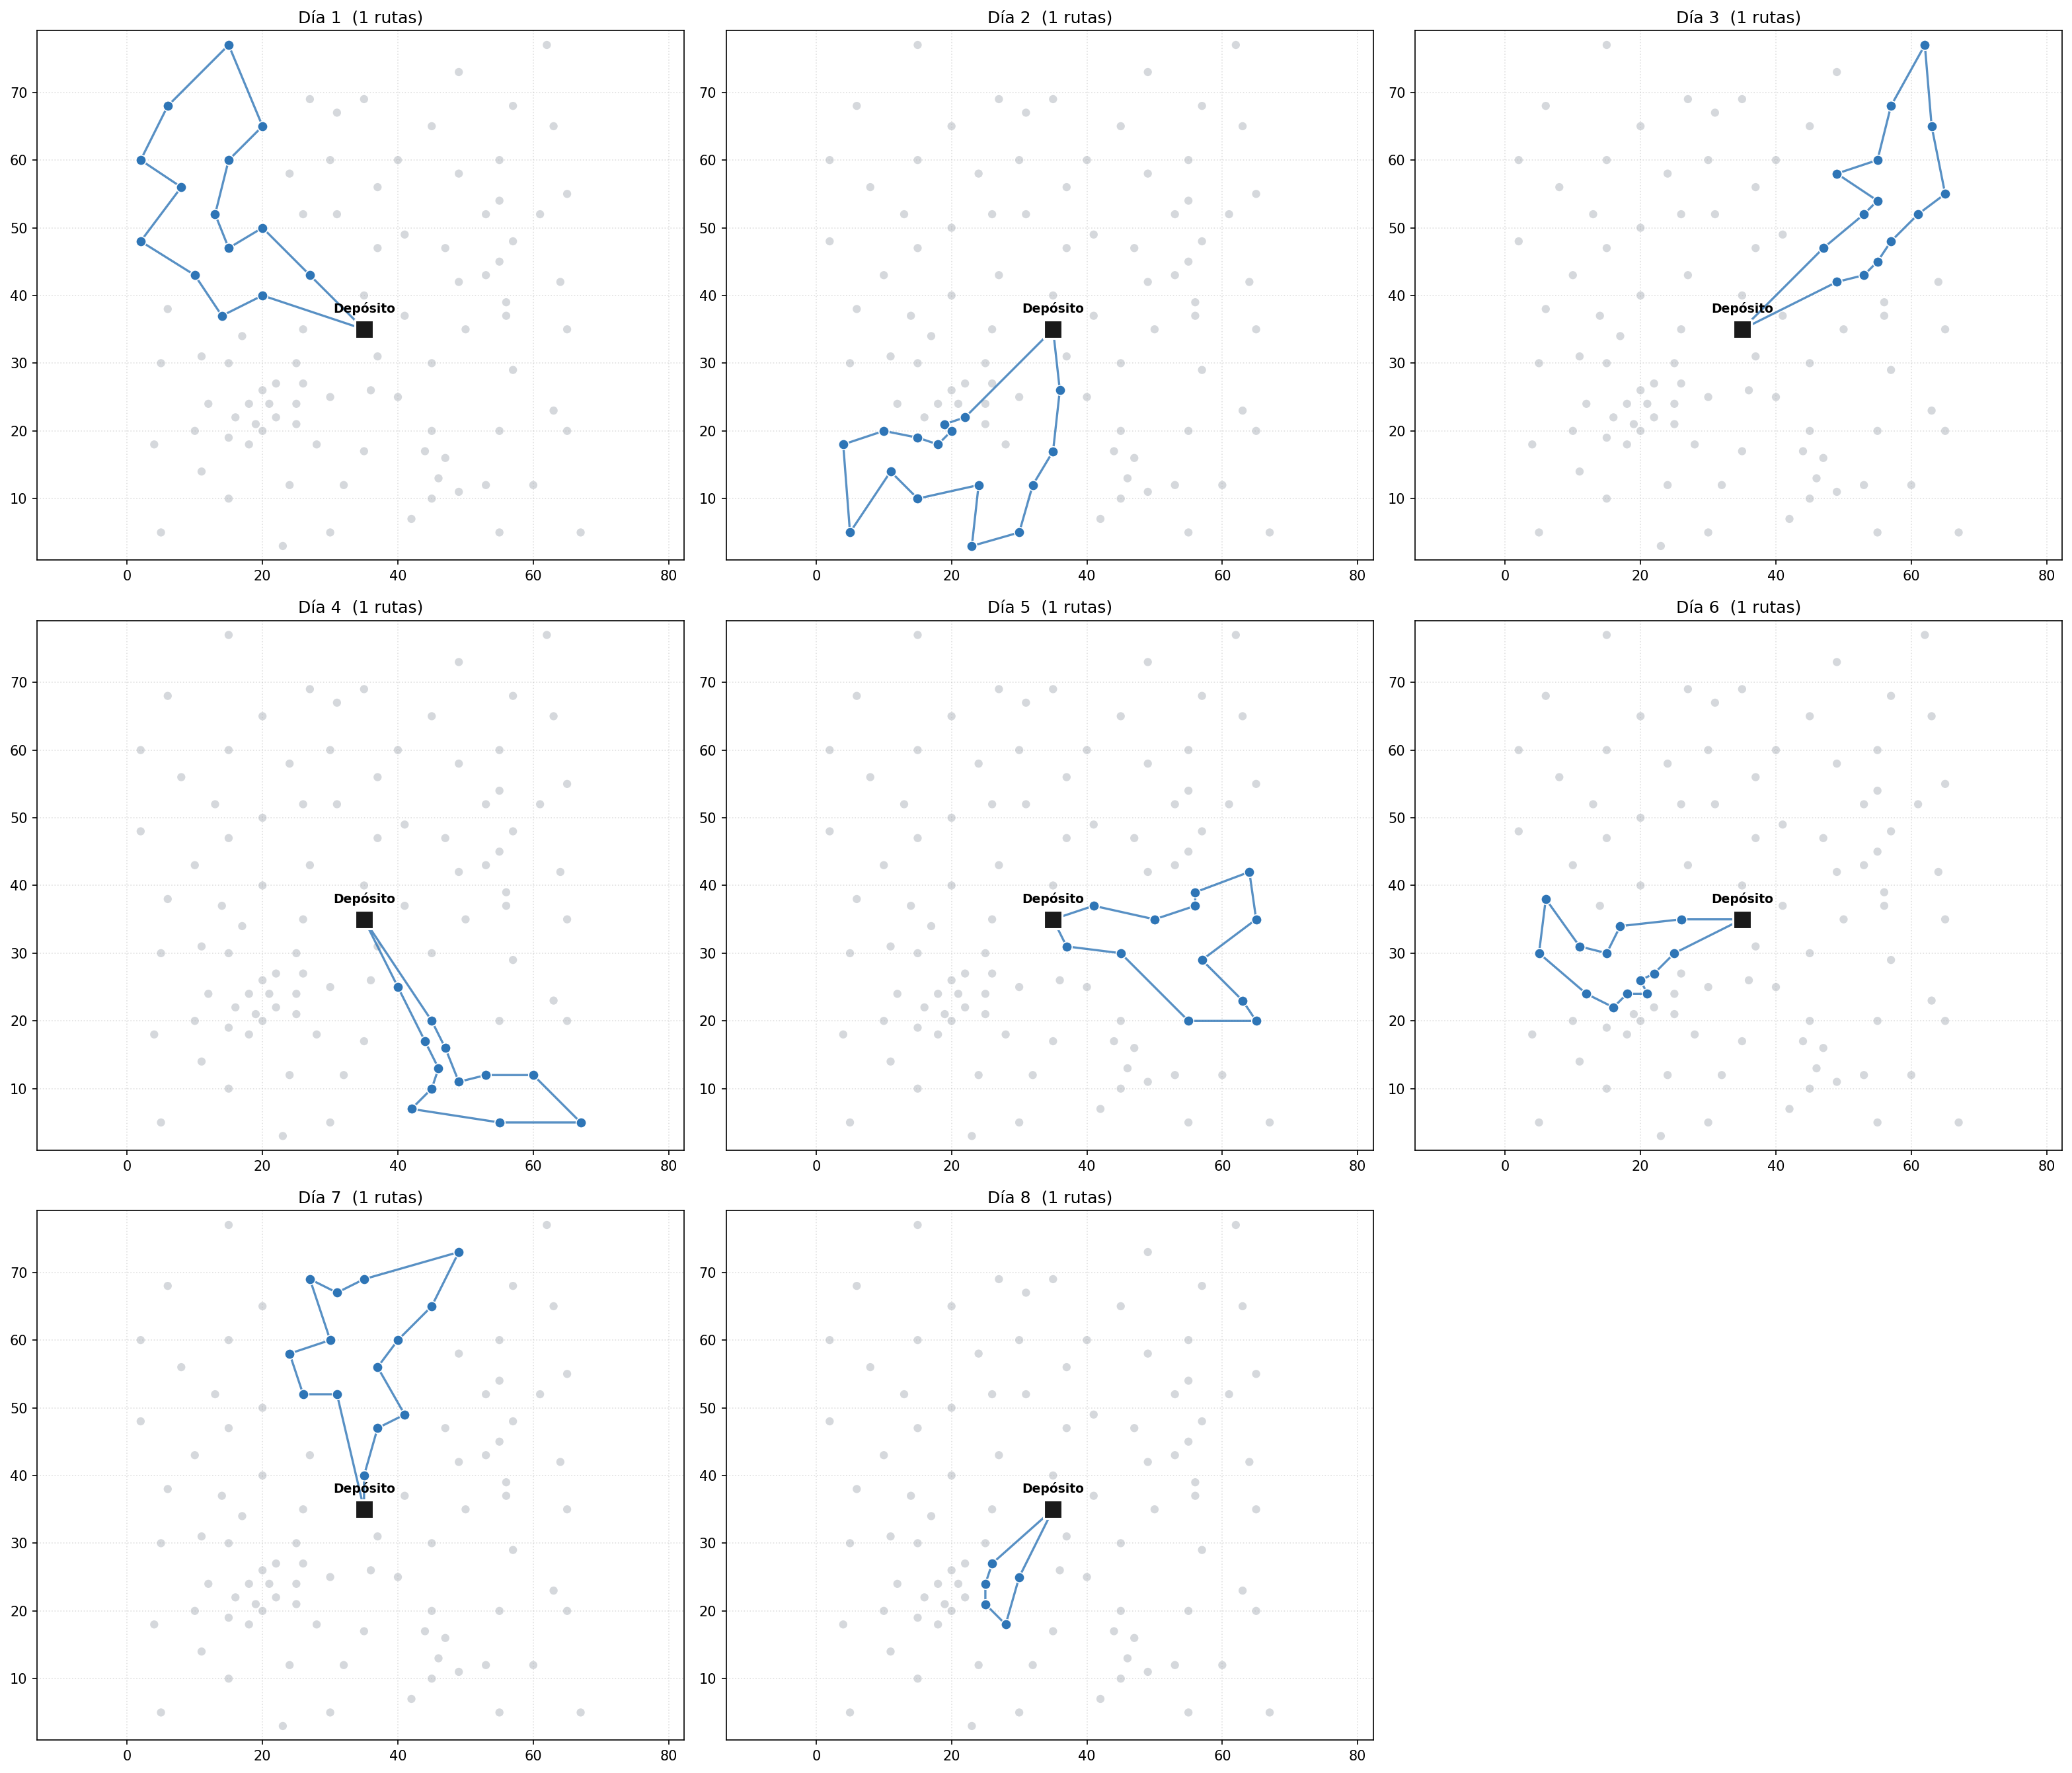
\includegraphics[
        width=\linewidth,
        height=0.80\textheight,
        keepaspectratio
    ]{figures/rutas_p09_BKS.png}
    \caption{Mejor solución conocida (BKS) para la instancia $p09$: costo $826{,}1$.}
    \caption*{Fuente: Elaboración propia.}
    \label{fig:rutas-p09-bks}
\end{figure}

\javi{Profe, arreglé los captions de p06 y p09: ahora cada parte (RL y BKS) tiene su propio caption y label, ninguna queda vacía. También cambié "mejores soluciones" por "soluciones representativas" para ser consistente con lo que aclaré en p01.}

%=============================================================%
\subsection{Identificación de los límites del método} \label{sec:limites}
%=============================================================%
Poner a prueba el modelo también implicó llevarlo hasta sus puntos de quiebre. Este proceso permitió identificar dos límites claros en el enfoque propuesto, los cuales se documentan y analizan a continuación.

%=============================================================%
\subsubsection{Límite combinatorio: familia B}
Al evaluar la instancia $p02$ (familia B, $50$ clientes, horizonte 5 días y 3 vehículos con multi-frecuencia), el patrón fue inequívoco: las cinco semillas entrenadas resultaron \emph{infactibles}, dejando clientes sin atender. La Tabla~\ref{tab:p02-detalle} muestra el detalle, incluyendo al VNS como referencia de un método que sí resuelve la instancia.

\begin{table}[H]
    \centering
    \caption{\label{tab:p02-detalle} Detalle multi-semilla sobre la instancia $p02$. Todas las semillas del agente resultan infactibles.}
    \caption*{Fuente: Elaboración propia.}
    \renewcommand{\arraystretch}{1.15}
    \setlength{\tabcolsep}{10pt}
    \begin{tabular}{@{}lccc@{}}
        \toprule
        \textbf{Semilla} & \textbf{Costo} & \textbf{Gap (\%)} & \textbf{Factibilidad} \\
        \midrule
        $0$ & $2038{,}28$ & $+54{,}1$ & infactible \\
        $1$ & $1955{,}38$ & $+47{,}8$ & infactible \\
        $2$ & $2068{,}85$ & $+56{,}4$ & infactible \\
        $3$ & $1961{,}22$ & $+48{,}3$ & infactible \\
        $4$ & $1514{,}45$ & $+14{,}5$ & infactible \\
        \midrule
        VNS (referencia) & $1587{,}71$ & $+20{,}0$ & factible \\
        \bottomrule
    \end{tabular}
\end{table}

A nivel técnico, es crucial aclarar que el costo y el gap reportados para estas semillas infactibles corresponden únicamente al costo de las rutas parciales que el agente logró construir, las cuales no cubren el total de la demanda. Por lo tanto, estos valores no se pueden comparar directamente con el gap de una solución completa como la de VNS. Por ejemplo, que la semilla $4$ tenga un gap aparentemente bajo ($+14{,}5\%$) no significa que sea una solución casi tan buena como VNS; es más barata simplemente porque omitió visitar a ciertos clientes. Para evitar interpretaciones erróneas, la columna de factibilidad siempre debe leerse en conjunto con el gap.

Tanto el VNS ($+20{,}0\%$, factible) como la heurística Greedy resuelven esta misma instancia sin dificultad, generando soluciones que cubren la totalidad de la demanda (sus resultados completos figuran en la Tabla~\ref{tab:consolidada}). Queda comprobado, entonces, que el problema sí admite una solución válida, y la falla es atribuible estrictamente a la naturaleza del agente y no a una imposibilidad estructural de la instancia.

El diagnóstico de la causa descarta una hipótesis inicial de saturación de capacidad: $p02$ tiene una saturación de $86\%$, menor que la de $p03$ ($97\%$), que sí se resuelve. La diferencia estructural relevante es la combinación de multi-frecuencia con múltiples vehículos por día: en $p02$ el agente debe coordinar simultáneamente qué clientes visitar, en qué días repetir las visitas y cómo distribuir la carga entre tres vehículos. Esta combinación de decisiones acopladas excede la capacidad del enfoque constructivo sin retroceso. \eli{¿Acá no hay BKS ó greedy?} \javi{Profe, dejé la tabla con RL + VNS para no saturarla, pero agregué en el texto que Greedy también resuelve p02 (sus datos completos, junto al BKS, están en la tabla consolidada). El punto clave es que ambos baselines la resuelven, así que la infactibilidad es del agente, no del problema.}

%=============================================================%
\subsubsection{Límite por saturación extrema: $p06$ semilla 4}
El segundo límite apareció en la instancia $p06$ (familia C, $75$ clientes, horizonte de 10 días, un vehículo y saturación $97\%$). En este caso, cuatro de las cinco semillas produjeron soluciones factibles con un desempeño muy consistente (gaps entre $+51{,}9\%$ y $+57{,}9\%$), pero la semilla $4$ resultó infactible. Es la única instancia del estudio donde la factibilidad cae del $100\%$ a un $4/5$.

A diferencia de lo que ocurre en $p02$, donde la falla es absoluta y sistemática, en $p06$ la infactibilidad es apenas ocasional. Esto indica un límite mucho menos rígido, provocado por la altísima exigencia de combinar una saturación extrema de capacidad con un horizonte de planificación muy largo (10 días). En estas condiciones de borde, el método mantiene su capacidad para encontrar rutas válidas en la gran mayoría de los intentos, pero pierde la garantía de factibilidad universal.

%=============================================================%
\subsection{Generalización} \label{subsec:generalizacion}
%=============================================================%
Como se definió en la Sección~\ref{sec:Metodosdeevaluacion}, el objetivo del eje de generalización es determinar si la política aprendida realmente captura principios de ruteo transferibles, o si simplemente se dedica a memorizar la secuencia de decisiones específica de la instancia con la que entrenó. Para responder a esta pregunta, se estructuraron dos experimentos utilizando las instancias de $50$ clientes ($p01$, $p02$, $p03$). Al compartir exactamente la misma dimensión de estado y de acciones, estas instancias permiten hacer una comparación controlada sin necesidad de recurrir a técnicas de relleno paramétrico.

Antes de interpretar los resultados, hay un detalle estructural clave a considerar: $p01$ (familia A) y $p03$ (familia C), pese a pertenecer a familias distintas, comparten exactamente la misma geometría de clientes. Tienen las mismas coordenadas, demandas y frecuencias de visita (todas iguales a 1). La única diferencia real entre ambas es el horizonte temporal y la cantidad de vehículos ($T{=}2, K{=}3$ en $p01$, frente a $T{=}5, K{=}1$ en $p03$). Esto convierte el cruce de modelos entre estas dos instancias en una prueba relevante, pues no se evalúa si el agente reconoce un mapa nuevo, sino si es capaz de adaptar su comportamiento a una configuración logística completamente distinta operando sobre el mismo espacio geográfico.

Es importante aclarar que los resultados de esta sección provienen de una única corrida por configuración, obtenida durante una fase exploratoria previa a la adopción del protocolo de cinco semillas del resto del capítulo. La razón es que estos experimentos de generalización tienen un carácter cualitativo: su objetivo no es cuantificar con precisión estadística el gap, sino inspeccionar el mecanismo de decisión del agente al enfrentarse a instancias no vistas. Como se detalla a continuación, las conclusiones se sustentan en el análisis directo de la secuencia de acciones paso a paso, y no en el valor agregado del costo, por lo que son robustas pese a provenir de una sola corrida. \eli{¿por qué?} \javi{Profe, aclaré el porqué: estos experimentos son cualitativos (miran el mecanismo de decisión paso a paso, no el número final), y por eso una corrida basta para la conclusión. La validación estadística con multi-semilla queda como trabajo futuro, lo menciono más abajo.}

Los hallazgos cualitativos que se describen a continuación son robustos, ya que se verificaron analizando directamente la secuencia de decisiones del agente paso a paso y no solo el costo agregado. No obstante, su validación estadística formal mediante múltiples semillas queda propuesta como trabajo futuro.

%=============================================================%
\subsubsection{Transferencia cero-shot}
La Tabla~\ref{tab:cero-shot} muestra qué ocurre al evaluar a los agentes especializados en $p01$ y en $p03$ directamente sobre las instancias que no vieron durante su entrenamiento, sin ningún tipo de reajuste o reentrenamiento previo. En palabras simples, esto corresponde a una evaluación cero-shot\footnote{En el ámbito del aprendizaje automático, la transferencia zero-shot o cero-shot consiste en someter a un modelo ya entrenado a un escenario o tarea completamente nueva, comprobando su capacidad de generalizar sin realizar ninguna actualización adicional en los parámetros de su red neuronal.}.

\begin{table}[H]
    \centering
    \caption{\label{tab:cero-shot} Transferencia cero-shot entre $p01$, $p02$ y $p03$. El agente evaluado sobre su propia instancia de entrenamiento se marca como referencia.}
    \caption*{Fuente: Elaboración propia.}
    \small
    \renewcommand{\arraystretch}{1.15}
    \setlength{\tabcolsep}{10pt}
    \begin{tabular}{@{}llcc@{}}
        \toprule
        \textbf{Agente} & \textbf{Evaluado en} & \textbf{Gap vs BKS} & \textbf{Factible} \\
        \midrule
        Especializado en $p01$ & $p01$ (referencia)     & $+17{,}7\%$ & sí \\
        Especializado en $p01$ & $p03$ (transferencia)  & $+17{,}7\%$ & sí \\
        Especializado en $p01$ & $p02$ (transferencia)  & $+25{,}6\%$ & NO \\
        \midrule
        Especializado en $p03$ & $p03$ (referencia)     & $+21{,}3\%$ & sí \\
        Especializado en $p03$ & $p01$ (transferencia)  & $+20{,}1\%$ & sí \\
        Especializado en $p03$ & $p02$ (transferencia)  & $+23{,}7\%$ & NO \\
        \bottomrule
    \end{tabular}
\end{table}

A simple vista, las transferencias cruzadas entre $p01$ y $p03$ parecen un éxito rotundo. En ambos casos la política mantiene la factibilidad y logra un gap casi idéntico al de su propia instancia de entrenamiento. Sin embargo, al revisar paso a paso las decisiones que tomó el agente (en lugar de mirar solo el costo final), se descubrió que detrás de estos números operan mecanismos completamente distintos, lo cual cambia drásticamente lo que se puede afirmar sobre la generalización del modelo.

Al llevar el agente especializado de $p01$ a $p03$, la secuencia completa de acciones que ejecutó resultó ser idéntica, paso a paso, a la que hizo en $p01$. Armó exactamente la misma partición de rutas y, por ende, obtuvo el mismo costo ($617{,}39$). Esto ocurre porque la estructura del entorno de simulación (el horizonte y el número de vehículos) limita el presupuesto máximo de rutas ($T \times K$), pero no impide al agente tomar sus decisiones habituales si no excede ese límite. La solución memorizada por el agente requería exactamente cinco rutas, lo cual cuadraba por mera casualidad con el presupuesto de ambas configuraciones (6 rutas posibles en $p01$, 5 rutas en $p03$). Por lo tanto, esta coincidencia no es evidencia de adaptación al contexto logístico. Es un caso de transferencia contingente, es decir, la política actuó de forma ciega ante el horizonte y los vehículos, y la solución resultó factible solo por \enquote{suerte} geométrica.

El caso inverso, el agente especializado en $p03$ evaluado en $p01$, es cualitativamente opuesto. Aquí, la secuencia de acciones diverge de su comportamiento original en $p03$ justo a partir del paso 22. Este es exactamente el instante en el que la variable de estado que codifica el vehículo activo comienza a ser distinta entre ambas instancias. $p01$ permite usar hasta tres vehículos por día, mientras que $p03$ obliga a cambiar de día tras usar uno. Al notar esta diferencia en el estado, el agente construye una configuración de rutas distinta, manteniendo la factibilidad y logrando incluso un mejor gap ($+20{,}1\%$ frente a $+21{,}3\%$). Esto sí constituye evidencia de adaptación genuina, es decir, la red neuronal leyó correctamente el contexto logístico del estado y modificó su estrategia sobre la marcha para ajustarse a las nuevas reglas.

Como era de esperarse, en ambos sentidos de transferencia la instancia $p02$ resultó infactible (gaps de $+25{,}6\%$ y $+23{,}7\%$). Esto refuerza el límite combinatorio documentado en la Sección~\ref{sec:limites}: ni siquiera un agente entrenado en otra instancia es capaz de sortear la barrera de coordinar multi-frecuencia con múltiples vehículos bajo esta arquitectura constructiva.

%=============================================================%
\subsubsection{Entrenamiento multi-instancia}
El segundo experimento consistió en entrenar a un solo agente sobre las tres instancias de $50$ clientes de forma simultánea. En la práctica, durante el entrenamiento el agente no se enfrenta siempre a la misma instancia, sino que estas se van rotando: en cada episodio se le presenta una de las tres ($p01$, $p02$ o $p03$), de modo que a lo largo del entrenamiento acumula experiencia sobre todas ellas. La hipótesis era que esta exposición a múltiples instancias produciría una política más robusta y generalizable que la de un agente especializado en una sola. La Tabla~\ref{tab:multi-instancia} muestra los resultados. \eli{esta parte no la entiendo.} \javi{Profe, reformulé la explicación: el entrenamiento multi-instancia significa que en cada episodio el agente entrena sobre una de las tres instancias (rotándolas), para que aprenda de todas a la vez. Antes decía "alternando cíclicamente" que era confuso.}

\begin{table}[H]
    \centering
    \caption{\label{tab:multi-instancia} Desempeño del agente entrenado bajo el esquema multi-instancia.}
    \caption*{Fuente: Elaboración propia.}
    \renewcommand{\arraystretch}{1.15}
    \setlength{\tabcolsep}{11pt}
    \begin{tabular}{@{}ccc@{}}
        \toprule
        \textbf{Instancia evaluada} & \textbf{Gap vs BKS} & \textbf{Factible} \\
        \midrule
        $p01$ & $+94{,}4\%$ & sí \\
        $p02$ & $+58{,}5\%$ & NO \\
        $p03$ & $+85{,}5\%$ & sí \\
        \bottomrule
    \end{tabular}
\end{table}

Los resultados contrastan drásticamente con los agentes especializados. En $p01$, el gap del agente multi-instancia se disparó a $+94{,}4\%$ (casi cinco veces peor que el $+17{,}7\%$ original). En $p03$, la caída es igual de severa ($+85{,}5\%$ frente a $+21{,}3\%$). La razón detrás de esta degradación radica en la heterogeneidad estructural del entrenamiento. Mientras $p01$ exige optimizar dos días con tres vehículos, $p03$ impone cinco días con un solo vehículo. Al obligar a una única red a asimilar dinámicas temporales tan dispares, la política termina diluyendo su capacidad de representación. En lugar de volverse experta en un problema, alcanza un desempeño mediocre en todos. Esto se confirma al revisar la tasa de episodios factibles durante su entrenamiento: el agente multi-instancia se estancó entre un $56\%$ y un $60\%$, muy por debajo del prácticamente $100\%$ que alcanzan rápidamente los agentes especialistas.

%=============================================================%
\subsubsection{Síntesis del eje de generalización}
La transferencia contingente, la adaptación genuina y el colapso del entrenamiento multi-instancia entregan una respuesta llena de matices. El agente efectivamente es capaz de generalizar su comportamiento a configuraciones logísticas nuevas cuando logra percibir la diferencia en su vector de estado (caso $p03 \rightarrow p01$). Sin embargo, también demostró que puede arrojar resultados aparentemente exitosos por motivos ajenos al aprendizaje (caso $p01 \rightarrow p03$), lo que subraya lo importante que es inspeccionar siempre los mecanismos de la red neuronal y no confiarse únicamente en un buen número en el costo final.

Por otro lado, obligar al agente a generalizar mediante un entrenamiento multi-instancia sacrificó fuertemente la calidad de sus soluciones, evidenciando una fuerte tensión entre especialización y generalización, algo muy característico del Aprendizaje por Refuerzo en optimización combinatoria~\cite{nazari2018reinforcementlearningsolvingvehicle}.

%=============================================================%
\subsection{Comparación global con los baselines} \label{sec:comparacion-global}
%=============================================================%
La Tabla~\ref{tab:consolidada} consolida los resultados de los tres métodos sobre las nueve instancias evaluadas, y la Figura~\ref{fig:barras-comparativo} permite visualizarlos de forma directa. En este gráfico y en la tabla, las instancias $p05$ y $p08$ figuran como \enquote{no evaluado} para el agente RL. Esta decisión se sustenta en dos motivos técnicos y prácticos. Primero, la evaluación previa de $p02$ ($50$ clientes, familia B) resultó infactible en sus cinco semillas, evidenciando un claro límite combinatorio. Como $p05$ y $p08$ comparten exactamente las mismas características estructurales (horizonte medio, múltiples vehículos por día y patrones multi-frecuencia coordinados), el resultado esperable sería análogo o peor. Segundo, el entrenamiento con la red ampliada ($[512, 512]$, $500\,000$ pasos) exige cerca de dos horas de cómputo por instancia para completar las cinco semillas. Por lo tanto, se priorizaron esos recursos para escalar las familias donde el método sí alcanza factibilidad ($p04$, $p06$, $p07$, $p09$) y entender mejor su verdadero rango de aplicabilidad. Por su parte, los métodos Greedy y VNS sí se ejecutaron en toda la familia B, confirmando que estas instancias admiten soluciones factibles mediante heurísticas clásicas.

\begin{table}[H]
    \centering
    \caption{\label{tab:consolidada} Resultados consolidados sobre las nueve instancias del conjunto NEO evaluadas. Gap respecto a la mejor solución conocida, en porcentaje. El agente RL se reporta como media sobre semillas factibles.}
    \caption*{Fuente: Elaboración propia.}
    \small
    \renewcommand{\arraystretch}{1.15}
    \setlength{\tabcolsep}{7pt}
    \begin{tabular}{@{}cccccc@{}}
        \toprule
        \textbf{Familia} & \textbf{Instancia} & \textbf{Greedy} & \textbf{VNS} & \textbf{RL} & \textbf{Factib. RL} \\
        \midrule
        \multirow{3}{*}{A} & $p01$ &  $+70{,}2\%$ &  $+31{,}7\%$ & $+19{,}7\%$  & $5/5$ \\
                           & $p04$ & $+212{,}8\%$ &  $+23{,}1\%$ & $+53{,}9\%$  & $5/5$ \\
                           & $p07$ &  $+75{,}1\%$ &  $+27{,}3\%$ & $+57{,}4\%$  & $5/5$ \\
        \midrule
        \multirow{3}{*}{B} & $p02$ &  $+44{,}0\%$ &  $+20{,}0\%$ & infactible   & $0/5$ \\
                           & $p05$ &  $+53{,}9\%$ &  $+17{,}0\%$ & no evaluado  & --- \\
                           & $p08$ &  $+52{,}9\%$ &  $+18{,}3\%$ & no evaluado  & --- \\
        \midrule
        \multirow{3}{*}{C} & $p03$ & $+100{,}2\%$ &  $+83{,}8\%$ & $+28{,}0\%$  & $5/5$ \\
                           & $p06$ & $+118{,}5\%$ & $+104{,}7\%$ & $+55{,}7\%$  & $4/5$ \\
                           & $p09$ & $+156{,}9\%$ & $+128{,}5\%$ & $+66{,}7\%$  & $5/5$ \\
        \bottomrule
    \end{tabular}
\end{table}

\begin{figure}[H]
    \centering
    \begin{tikzpicture}
        \begin{axis}[
            width=10.8cm,
            height=7cm,
            ybar=2pt,
            bar width=6pt,
            ylabel={Gap respecto al BKS (\%)},
            symbolic x coords={p01,p02,p03,p04,p05,p06,p07,p08,p09},
            xtick=data,
            ymin=0,
            ymax=230,
            ytick={0,50,100,150,200},
            grid=major,
            xmajorgrids=true,
            ymajorgrids=true,
            grid style={line width=0.3pt, draw=gray!30},
            axis line style={black!70},
            tick style={black!70},
            tick label style={font=\small},
            label style={font=\small},
            enlarge x limits=0.10,
            legend style={
                font=\small,
                draw=black!40,
                fill=white,
                rounded corners=2pt,
                at={(1.04,0.5)},
                anchor=west
            },
            legend cell align=left,
            clip=false
        ]
            \addplot[draw=greedyLine, fill=greedyFill] coordinates {
                (p01,70.2) (p02,44.0) (p03,100.2) (p04,212.8)
                (p05,53.9) (p06,118.5) (p07,75.1) (p08,52.9) (p09,156.9)
            };
            \addlegendentry{Greedy}

            \addplot[draw=vnsLine, fill=vnsFill] coordinates {
                (p01,31.7) (p02,20.0) (p03,83.8) (p04,23.1)
                (p05,17.0) (p06,104.7) (p07,27.3) (p08,18.3) (p09,128.5)
            };
            \addlegendentry{VNS}

            \addplot[draw=rlLine, fill=rlFill] coordinates {
                (p01,19.7) (p03,28.0) (p04,53.9)
                (p06,55.7) (p07,57.4) (p09,66.7)
            };
            \addlegendentry{RL}
        \end{axis}
    \end{tikzpicture}
    \caption{Comparación del gap respecto al BKS de los tres métodos sobre las instancias evaluadas. Las instancias $p02$, $p05$ y $p08$ (familia B) no presentan barra de RL por resultar infactibles o no evaluadas.}
    \caption*{Fuente: Elaboración propia.}
    \label{fig:barras-comparativo}
\end{figure}

El análisis global de estos datos revela tres escenarios operativos muy claros:

\begin{itemize}
    \item En $50$ clientes (familias A y C), el agente RL supera a VNS: logra $+19{,}7\%$ frente a $+31{,}7\%$ en $p01$, y un aplastante $+28{,}0\%$ frente a $+83{,}8\%$ en $p03$.

    \item En $75$ y $100$ clientes (familias A y C), VNS supera al RL: por ejemplo, logra un $+23{,}1\%$ frente al $+53{,}9\%$ del agente en $p04$. Esto ocurre porque el refinamiento local del VNS rinde mucho más al crecer la instancia, mientras que el enfoque puramente constructivo del RL pierde calidad geométrica.

    \item En la familia B, VNS logra resolver el problema mientras el RL no alcanza la factibilidad, un límite combinatorio que se mantiene incluso al intentar aplicar transferencia de aprendizaje desde otras instancias.
\end{itemize}

Sin embargo, este panorama cambia drásticamente al analizar los tiempos de inferencia, donde el agente RL demuestra una superioridad absoluta. La Tabla~\ref{tab:tiempos} y la Figura~\ref{fig:tiempos} resumen el tiempo de ejecución requerido por cada método en las distintas instancias.

\begin{table}[H]
    \centering
    \caption{\label{tab:tiempos} Tiempos de inferencia/ejecución de los tres métodos por instancia.}
    \caption*{Fuente: Elaboración propia.}
    \renewcommand{\arraystretch}{1.15}
    \setlength{\tabcolsep}{10pt}
    \begin{tabular}{@{}cccc@{}}
        \toprule
        \textbf{Instancia} & \textbf{Greedy} & \textbf{VNS} & \textbf{RL (inferencia)} \\
        \midrule
        $p01$ & $0{,}007$ s & $3{,}368$ s & $\sim 0{,}04$ s \\
        $p02$ & $0{,}010$ s & $5{,}110$ s & $\sim 0{,}04$ s \\
        $p03$ & $0{,}006$ s & $0{,}239$ s & $\sim 0{,}04$ s \\
        $p04$ & $0{,}019$ s & $5{,}346$ s & $\sim 0{,}06$ s \\
        $p05$ & $0{,}026$ s & $11{,}842$ s & --- \\
        $p06$ & $0{,}012$ s & $0{,}330$ s & $\sim 0{,}06$ s \\
        $p07$ & $0{,}036$ s & $21{,}897$ s & $\sim 0{,}08$ s \\
        $p08$ & $0{,}077$ s & $38{,}740$ s & --- \\
        $p09$ & $0{,}023$ s & $0{,}840$ s & $\sim 0{,}08$ s \\
        \bottomrule
    \end{tabular}
\end{table}

\begin{figure}[H]
    \centering
    \begin{tikzpicture}
        \begin{semilogyaxis}[
            width=10.8cm,
            height=7cm,
            ylabel={Tiempo (segundos, escala logarítmica)},
            symbolic x coords={p01,p02,p03,p04,p05,p06,p07,p08,p09},
            xtick=data,
            ymin=0.001,
            ymax=100,
            ytick={0.001,0.01,0.1,1,10,100},
            grid=major,
            xmajorgrids=true,
            ymajorgrids=true,
            grid style={line width=0.3pt, draw=gray!30},
            axis line style={black!70},
            tick style={black!70},
            tick label style={font=\small},
            label style={font=\small},
            enlarge x limits=0.10,
            legend style={
                font=\small,
                draw=black!40,
                fill=white,
                rounded corners=2pt,
                at={(1.04,0.5)},
                anchor=west
            },
            legend cell align=left,
            clip=false
        ]
            \addplot[color=greedyLine, thick, mark=square*, mark size=2.4pt]
            coordinates {
                (p01,0.007) (p02,0.010) (p03,0.006) (p04,0.019)
                (p05,0.026) (p06,0.012) (p07,0.036) (p08,0.077) (p09,0.023)
            };
            \addlegendentry{Greedy}

            \addplot[color=vnsLine, thick, mark=triangle*, mark size=2.8pt]
            coordinates {
                (p01,3.368) (p02,5.110) (p03,0.239) (p04,5.346)
                (p05,11.842) (p06,0.330) (p07,21.897) (p08,38.740) (p09,0.840)
            };
            \addlegendentry{VNS}

            \addplot[color=rlLine, thick, mark=*, mark size=2.8pt]
            coordinates {
                (p01,0.04) (p02,0.04) (p03,0.04) (p04,0.06)
                (p06,0.06) (p07,0.08) (p09,0.08)
            };
            \addlegendentry{RL}
        \end{semilogyaxis}
    \end{tikzpicture}
    \caption{Tiempos de inferencia de los tres métodos por instancia, en escala logarítmica.}
    \caption*{Fuente: Elaboración propia.}
    \label{fig:tiempos}
\end{figure}

Queda en evidencia que el agente entrega su solución entre uno y dos órdenes de magnitud más rápido que VNS. En instancias grandes (como $p07$), donde el VNS requiere decenas de segundos para terminar su proceso, el agente entrenado responde en menos de una décima de segundo. Esta ventaja resulta de suma importancia para escenarios operativos reales, donde el costo logístico de la ruta debe equilibrarse con la necesidad de obtener tiempos de respuesta casi inmediatos.

Los tiempos reportados hasta ahora corresponden a la fase de inferencia; el entrenamiento del agente constituye una inversión de cómputo previa y única por instancia. La configuración base ($300\,000$ pasos, red $[256,256]$) requirió aproximadamente $9$ minutos por semilla en CPU estándar, sumando cerca de $45$ minutos por instancia bajo el protocolo multi-semilla. La configuración escalada ($500\,000$ pasos, red $[512,512]$) requirió aproximadamente $20$ minutos por semilla, es decir, cerca de $100$ minutos por instancia. En agregado, los siete análisis multi-semilla completos totalizaron alrededor de $7$ horas de cómputo. Es relevante destacar que este costo se paga una única vez: una vez entrenado, el agente resuelve nuevas ejecuciones de la misma instancia en fracciones de segundo, lo que sostiene su ventaja operativa frente a VNS en escenarios de uso repetido o de respuesta rápida. Cabe subrayar, además, que todo el entrenamiento se ejecutó sin aceleración por GPU, lo que refuerza la accesibilidad del método en infraestructura de cómputo convencional. 

\eli{Hablar de tiempos de entrenamiento.} 
\javi{Profe, agregué el párrafo de tiempos de entrenamiento con datos reales: ~9 min/semilla en config base, ~20 min/semilla en escalada, ~7 horas agregadas, todo en CPU sin GPU. El punto clave es que es un costo único (se entrena una vez y luego infiere instantáneo), a diferencia de VNS que repite su búsqueda cada vez.}

%=============================================================%
\subsection{Síntesis de la validación} \label{sec:sintesis-validacion}
%=============================================================%
La Tabla~\ref{tab:sintesis-familias} resume los hallazgos agrupados por familia estructural, incorporando además las observaciones del eje de generalización.

\begin{table}[H]
    \centering
    \caption{\label{tab:sintesis-familias} Síntesis de los resultados por familia estructural.}
    \caption*{Fuente: Elaboración propia.}
    \small
    \renewcommand{\arraystretch}{1.18}
    \setlength{\tabcolsep}{7pt}
    \begin{tabularx}{\textwidth}{@{}>{\centering\arraybackslash}p{1.5cm}XX@{}}
        \toprule
        \textbf{Familia} & \textbf{Calidad y robustez} & \textbf{Generalización} \\
        \midrule
        A & Factibilidad universal ($15/15$ corridas). Supera a VNS en $50$ clientes ($p01$); VNS supera al RL en $75$ y $100$ clientes ($p04$, $p07$). Degradación predecible al escalar. & Transferencia hacia $p03$ (familia~C, misma geometría): contingente en un sentido, genuina en el otro. \\
        \midrule
        B & Infactibilidad sistemática en $p02$ ($0/5$ corridas factibles). Límite combinatorio identificado: el enfoque constructivo no coordina visitas multi-frecuencia entre múltiples vehículos. & Infactibilidad persiste bajo transferencia desde $p01$ y $p03$; el límite combinatorio es robusto a la estrategia de entrenamiento. \\
        \midrule
        C & Factibilidad alta ($14/15$ corridas). Supera a VNS en todas las escalas evaluadas con factibilidad ($p03$, $p06$, $p09$). Una infactibilidad ocasional en $p06$ semilla $4$. & Transferencia hacia $p01$ (familia~A, misma geometría): adaptación genuina verificada a nivel de secuencia de decisiones. \\
        \bottomrule
    \end{tabularx}
\end{table}

A partir de toda la evidencia recolectada a lo largo de este capítulo, se concluyen seis afirmaciones sobre el desempeño del modelo:

\begin{enumerate}
    \item \textbf{Superioridad inicial:} El agente supera al VNS en instancias de $50$ clientes (familias A y C), entregando mejores rutas en tiempos de inferencia que resultan ser entre uno y dos órdenes de magnitud menores.

    \item \textbf{Escalamiento robusto:} El método logra escalar a problemas de $75$ y $100$ clientes manteniendo una factibilidad casi universal ($29/30$ corridas factibles). Sin embargo, tal como evidencian los gráficos de rutas, pierde calidad geométrica relativa frente a la heurística de mejora local al aumentar la densidad de clientes.

    \item \textbf{Estabilidad operativa:} El comportamiento de la red neuronal es reproducible y predecible. La desviación estándar del gap entre las distintas semillas se mantuvo siempre acotada entre un $\pm 5\%$ y un $\pm 7\%$ en todas las configuraciones evaluadas.

    \item \textbf{Límite combinatorio transparente:} Se identificó una barrera técnica clara en la familia B. El agente puramente constructivo no logra coordinar decisiones de multi-frecuencia entre múltiples vehículos de forma simultánea, fallando en alcanzar la factibilidad en escenarios que el VNS resuelve con facilidad.

    \item \textbf{Velocidad de respuesta:} El agente ofrece una ventaja operativa sustancial en el tiempo de inferencia. En las instancias más grandes resuelve todo el ruteo en fracciones de segundo, posicionándolo como una alternativa altamente competitiva para entornos reales que exigen respuestas rápidas.

    \item \textbf{Generalización con matices:} Se comprobó que el agente no solo memoriza, sino que puede adaptar genuinamente su comportamiento a un nuevo contexto logístico si el vector de estado lo refleja ($p03 \rightarrow p01$). No obstante, también se descubrió que puede generar resultados \enquote{exitosos} por pura coincidencia geométrica ciega ($p01 \rightarrow p03$). Además, se confirmó que el entrenamiento multi-instancia genera una fuerte tensión con la especialización, degradando fuertemente el desempeño global del agente.
\end{enumerate}

Con esta validación, se demostró empíricamente que el enfoque basado en Aprendizaje por Refuerzo es competitivo, estable y extremadamente veloz dentro de su régimen de aplicabilidad. Al mismo tiempo, se delimitó con total transparencia las fronteras donde el modelo falla y requiere apoyo. Estos hallazgos preparan el terreno para el siguiente Capítulo, donde se plantearán las conclusiones finales de la memoria y se propondrán las líneas de trabajo futuro.
\newpage
\secnumbersection{CONCLUSIONES}

\javi{Profe! no se como citar los capítulos, intente colocando label al lado pero me cita la ultima seccion del capitulo anterior}
\eli{Me parece que es por cómo está redefinido el entorno. No rabees más con eso y déjalo fijo.}


Esta memoria abordó el desarrollo y la evaluación de un modelo basado en Aprendizaje por Refuerzo (RL) para la resolución del Problema de Ruteo de Vehículos Periódico (PVRP), planteado como una alternativa data-driven a las metaheurísticas clásicas que tradicionalmente han dominado la resolución de esta familia de problemas. El trabajo se estructuró en torno a la reformulación del PVRP como un Proceso de Decisión de Markov (MDP), permitiendo que un agente construya soluciones de manera secuencial mediante la interacción con un entorno de simulación, en lugar de depender de reglas de decisión diseñadas manualmente. La propuesta contempló cuatro componentes de diseño principales: 

\begin{itemize}
    \item La representación del estado como un vector de dimensión fija que integra información espacial y temporal.
    
    \item Un espacio de acciones discreto que incluye explícitamente la decisión de cerrar la ruta actual, otorgando al agente control directo sobre la estructura de la solución.
    
    \item Una función de recompensa con penalización proporcional al número de clientes no atendidos.
    
    \item Un mecanismo de enmascaramiento de acciones que garantiza la factibilidad local en cada paso de decisión, reduciendo el espacio de exploración durante el entrenamiento.
\end{itemize}
 
Sobre esta formulación se implementó un agente basado en el algoritmo Maskable PPO, entrenado y evaluado sobre nueve instancias del conjunto NEO~\cite{NEO2013} agrupadas en tres familias estructurales, con evaluación estadísticamente rigurosa mediante análisis multi-semilla sobre siete de esas instancias (cinco semillas cada una, para un total de treinta y cinco entrenamientos independientes), contrastada con dos métodos de referencia: una heurística voraz (Greedy) y la metaheurística Variable Neighborhood Search (VNS), reconocida en la literatura como uno de los métodos más efectivos para el PVRP~\cite{HEMMELMAYR2009791}. Adicionalmente, se evaluó la transferencia directa entre instancias y el entrenamiento conjunto sobre múltiples instancias, ejes que en conjunto permiten caracterizar no solo la calidad de las soluciones obtenidas, sino también la robustez estadística del método y su capacidad de generalización más allá de la instancia específica de entrenamiento.

Para evaluar el éxito de esta memoria, resulta fundamental contrastar los resultados obtenidos con los compromisos metodológicos iniciales. A lo largo del desarrollo, se cumplió con el objetivo general planteado en la propuesta original: desarrollar y evaluar un modelo basado en Aprendizaje por Refuerzo para la resolución del PVRP, con el propósito de determinar políticas de ruteo eficientes y adaptativas. Asimismo, se abordaron con éxito los cinco objetivos específicos comprometidos, logrando en varios casos superar ampliamente el alcance mínimo estipulado.

A continuación, se detalla el cumplimiento metodológico de cada uno de estos hitos:

\begin{itemize}
    \item \textbf{Revisión del estado del arte:} Este primer objetivo se realizó en el Capítulo~1 mediante una investigación bibliográfica profunda. Esta revisión abarcó desde los métodos exactos y heurísticos clásicos hasta los enfoques híbridos más recientes de Aprendizaje por Refuerzo aplicados al ruteo, lo que permitió situar la propuesta de esta memoria dentro de una línea de investigación científica altamente activa y en constante desarrollo.
    
    \item \textbf{Creación del entorno de simulación:} El segundo objetivo demandaba modelar adecuadamente las características y restricciones del PVRP. Para esto se materializó esta meta construyendo un entorno completamente funcional que reproduce de manera fiel el Proceso de Decisión de Markov descrito en el Capítulo~2. Con el fin de garantizar la robustez del software, se validó mediante $142$ pruebas automatizadas. Estas pruebas verifican estrictamente tanto las invariantes locales de factibilidad como la coherencia absoluta entre el costo acumulado y el costo oficial reportado por el conjunto NEO.
    
    \item \textbf{Desarrollo del agente funcional:} El tercer objetivo exigía un agente capaz de interactuar con el entorno y completar un ciclo de entrenamiento. Se realizó este hito implementando un agente basado en el algoritmo Maskable PPO. Calibrando este modelo de forma sistemática sobre la instancia base y, posteriormente, se recalibró para abordar escalas mayores. En esta etapa se superó el alcance mínimo estipulado en la propuesta original, ya que se diseñaron e incluyeron experimentos adicionales de transferencia y entrenamiento multi-instancia que no formaban parte de los compromisos iniciales.
    
    \item \textbf{Evaluación del modelo entrenado:} El cuarto objetivo apuntaba a medir el gap porcentual del modelo respecto al mejor resultado conocido (BKS). Esta tarea se abordó evaluando el agente sobre nueve instancias del conjunto NEO, cubriendo tres escalas de tamaño y tres familias estructurales distintas. Para otorgar un respaldo estadístico riguroso a los resultados, se utilizó una metodología multi-semilla, lo que permitió distinguir claramente el comportamiento reproducible del método frente a la variabilidad aleatoria propia de una corrida individual.
    
    \item \textbf{Comparación con baselines de la literatura:} Finalmente, el quinto objetivo requería contrastar la propuesta con métodos de resolución ya reportados. Este requisito se satisfizo mediante la implementación y ejecución de una heurística Greedy y de la metaheurística VNS sobre las nueve instancias de prueba. Con esto, se logró contrastar de forma exhaustiva la calidad de las soluciones, los tiempos de ejecución y las tasas de factibilidad en todos los escenarios, yendo mucho más allá de una simple validación sobre la instancia base.
\end{itemize}

Los experimentos realizados permiten exponer un conjunto de hallazgos centrales, todos sustentados estrictamente en la evidencia empírica reportada en el Capítulo~4. En primer lugar, destaca el rendimiento obtenido en las instancias de $50$ clientes pertenecientes a las familias A y C, donde el agente propuesto supera con claridad a la metaheurística VNS. Específicamente, en la instancia $p01$ el modelo de RL logra un gap medio de $+19{,}7\%$ (con una desviación de $\pm 6{,}5\%$ sobre cinco semillas), superando el $+31{,}7\%$ alcanzado por VNS. Esta superioridad se acentúa en la instancia $p03$, donde el gap del agente se sitúa en $+28{,}0\%$, marcando una diferencia notable frente al $+83{,}8\%$ de la metaheurística. Por su parte, la heurística voraz queda relegada a márgenes muy inferiores, registrando $+70{,}2\%$ y $+100{,}2\%$ en dichas instancias. Esta brecha de rendimiento confirma que el aprendizaje de una política basada en la experiencia acumulada aporta un valor analítico sustancial por sobre una regla de construcción miope. En consecuencia, se evidencia el alto valor de un enfoque aprendido para la construcción de rutas en escenarios de tamaño reducido.

Más allá de la calidad geométrica de las soluciones, el resultado más innovador de la evaluación radica en la eficiencia computacional durante la fase de inferencia. El agente entrega rutas completas entre uno y dos órdenes de magnitud más rápido que los métodos iterativos de comparación. Mientras que VNS requiere tiempos de ejecución que oscilan entre décimas de segundo y $38{,}7$ segundos dependiendo de la complejidad de la instancia, el modelo entrenado responde de manera consistente en apenas fracciones de segundo. Esta ventaja operativa trasciende el análisis académico y cobra particular relevancia en contextos operativos reales, donde la rapidez de respuesta condiciona directamente la viabilidad del despliegue tecnológico. En sistemas de planificación diaria en logística de distribución, la capacidad de recalcular rutas de forma instantánea ante cambios de última hora o contingencias en terreno resulta crítica, exigiendo tiempos de respuesta muy inferiores a los que una metaheurística iterativa tradicional puede ofrecer.

El método también escala estructuralmente a instancias de $75$ y $100$ clientes, manteniendo factibilidad en veintinueve de treinta corridas evaluadas (tasa global del $97\%$ en las familias A y C), aunque la calidad relativa al BKS se degrada con el tamaño: en la familia A, el gap medio pasa de $+19{,}7\%$ en $p01$ ($50$ clientes) a $+53{,}9\%$ en $p04$ ($75$ clientes) y $+57{,}4\%$ en $p07$ ($100$ clientes), con un patrón análogo en la familia C. El salto se produce principalmente entre $50$ y $75$ clientes, mientras que entre $75$ y $100$ la degradación se mitiga, sugiriendo una estabilización del método en esas escalas más que un deterioro indefinido a medida que crece la instancia. Este comportamiento es, además, reproducible: la desviación estándar del gap entre semillas se mantiene en el rango $\pm 5\%$ a $\pm 7\%$ en todas las configuraciones evaluadas, independientemente de la escala, lo que indica que los resultados observados no son producto del azar de una ejecución en particular sino una propiedad estable del método bajo la configuración adoptada, y permite descartar interpretaciones triunfalistas o pesimistas basadas en corridas individuales.

Junto a estas fortalezas, la evaluación identificó un límite combinatorio claro en la familia B: el agente no alcanza factibilidad en $p02$, instancia que el VNS resuelve sin dificultad ($+20{,}0\%$, factible; Sección~\ref{sec:limite-familiaB}). Descartada la saturación de capacidad como causa, dado que $p03$ posee saturación mayor y sí se resuelve, el fenómeno se atribuye a la naturaleza secuencial del enfoque constructivo sin retroceso, incapaz de coordinar simultáneamente la asignación multi-frecuencia y el reparto de carga entre múltiples vehículos. Los experimentos de transferencia confirmaron que este límite es robusto a la estrategia de entrenamiento, ya que persiste al evaluar sobre $p02$ agentes entrenados en otras instancias.

Los experimentos de transferencia directa (Sección~\ref{sec:transferencia}) entregaron uno de los hallazgos más matizados de esta investigación. Al evaluar cruzadamente los agentes especializados en $p01$ y $p03$, que comparten la geometría de clientes pero difieren en horizonte temporal y número de vehículos, se observaron dos regímenes opuestos. En el sentido $p01 \rightarrow p03$, la política reprodujo su solución paso a paso de forma ciega al nuevo contexto, produciendo el mismo costo ($617{,}39$) y resultando factible solo por coincidencia estructural entre el presupuesto de rutas de ambas configuraciones, lo que constituye una transferencia contingente y no una adaptación real. En el sentido inverso $p03 \rightarrow p01$, en cambio, la secuencia de decisiones divergió al percibir el cambio en la variable de estado que codifica el vehículo activo, construyendo una partición distinta que resultó factible e incluso mejoró el gap base ($+20{,}1\%$ frente a $+21{,}3\%$), lo que sí evidencia una adaptación genuina.

En conjunto, ambos experimentos demuestran que el agente es capaz de generalizar su comportamiento siempre y cuando la diferencia de contexto sea percibida correctamente por su representación de estado. Asimismo, dejan una lección metodológica de gran relevancia para la evaluación de sistemas de aprendizaje aplicados a la optimización combinatoria: resulta obligatorio inspeccionar el mecanismo secuencial detrás del costo final antes de catalogarlo como un aprendizaje transferible. Finalmente, a estos hallazgos se suma el análisis del entrenamiento conjunto sobre las tres instancias, denominado \texttt{ppo\_multi\_p01\_p02\_p03}. Si bien este enfoque produjo soluciones factibles en las familias A y C, experimentó una degradación de calidad muy significativa respecto a los agentes especializados, arrojando gaps que oscilaron entre el $+58\%$ y el $+94\%$. Esta caída en el rendimiento, equivalente a resultados aproximadamente cuatro veces peores, pone en evidencia la fuerte tensión existente entre la especialización y la generalización, una característica recurrente al aplicar algoritmos de RL en problemas de alta complejidad combinatoria.

Más allá de los resultados numéricos de calidad y generalización, el proceso de desarrollo del agente dejó dos lecciones metodológicas que resulta fundamental registrar explícitamente, pues ilustran la alta sensibilidad del comportamiento de un agente de Aprendizaje por Refuerzo frente a decisiones de diseño aparentemente secundarias. La primera de ellas se refiere a la calibración de hiperparámetros. Al utilizar los valores por defecto del algoritmo, consistentes en un coeficiente de entropía de $0{,}01$ y una red neuronal de $[128, 128]$ neuronas, la política convergía prematuramente hacia soluciones de baja calidad, quedando atrapada en óptimos locales tempranos. Fue necesario aumentar el coeficiente de entropía a $0{,}05$ para incentivar una exploración más prolongada, junto con ampliar la red a $[256, 256]$ neuronas para otorgar una mayor capacidad de representación al procesar el vector de estado del PVRP, logrando así la configuración que finalmente permitió superar a los métodos de referencia clásicos. Esta sensibilidad algorítmica confirma que, en la aplicación de modelos de aprendizaje a problemas de optimización combinatoria, la calibración de hiperparámetros trasciende de ser un detalle de afinación menor para convertirse en una condición estrictamente necesaria en la obtención de resultados competitivos. La segunda lección, de una relevancia aún mayor, surgió durante el desarrollo del entrenamiento multi-instancia y constituye un caso claro de vulneración de la recompensa o reward hacking. La función de recompensa original penalizaba la infactibilidad con un valor fijo, independientemente de la cantidad de clientes que quedaran sin atender, provocando que abandonar a un solo cliente costara computacionalmente lo mismo que abandonar a la totalidad de la demanda. El agente descubrió y explotó rápidamente este atajo, colapsando hacia soluciones triviales compuestas por una sola ruta y un único cliente visitado, lo que generaba un costo aparente mínimo pero producía una tasa de factibilidad que se desplomaba a cero. La corrección metodológica consistió en estructurar una penalización estrictamente proporcional al número de clientes no visitados, ajuste tras el cual la tasa de episodios factibles del entrenamiento multi-instancia ascendió y se estabilizó de forma sostenida, sin registrar nuevos colapsos. Este episodio ilustra un principio general crítico en el diseño de funciones de recompensa: el agente optimiza de manera literal la señal matemática que se le entrega y no la intención subyacente del diseñador, por lo que una penalización que no logra distinguir los grados de severidad frente a la violación de una restricción invita invariablemente al modelo a explotar el camino más barato para evadirla.

La rigurosidad científica exige delimitar con precisión los alcances de esta investigación y reconocer explícitamente las limitaciones del trabajo desarrollado. En términos de alcance empírico, se logró una caracterización estadísticamente robusta del agente sobre nueve instancias del conjunto NEO, abarcando tres escalas de tamaño y tres familias estructurales distintas bajo una implementación completamente reproducible. Esta reproducibilidad se garantiza mediante la disponibilidad de los modelos entrenados, un código de software respaldado por $142$ pruebas automatizadas y la capacidad de ejecutar la totalidad de los experimentos sobre hardware estándar sin requerir aceleración gráfica mediante GPU, lo que facilita la replicación del estudio sin depender de infraestructura computacional especializada. En cuanto a las limitaciones metodológicas, se constata que el agente construye las soluciones de forma estrictamente incremental sin contemplar una fase de mejora posterior. Esta carencia algorítmica se manifiesta visualmente en cruces de aristas que una optimización tradicional de tipo $2$-opt eliminaría con facilidad, lo que explica en gran medida la pérdida de calidad frente a la metaheurística VNS al escalar el tamaño de la red. Además, la arquitectura de la red neuronal opera sobre vectores de estado cuya dimensión está rígidamente ligada al número de clientes, impidiendo la transferencia directa de políticas aprendidas entre instancias de distinto tamaño sin someter al modelo a un reentrenamiento previo. Asimismo, la evaluación empírica se restringió al conjunto NEO estándar, marginando variantes más complejas que incluyen demandas estocásticas, ventanas de tiempo u otras restricciones dinámicas que son habituales en escenarios logísticos reales. Respecto a las limitaciones inherentes al enfoque de resolución propuesto, destaca el hecho de que el agente no logró alcanzar la factibilidad en la única instancia evaluada de la familia B, correspondiente a $p02$. Aunque las instancias $p05$ y $p08$ de esa misma categoría estructural no fueron entrenadas explícitamente debido al elevado costo computacional que demanda el protocolo multi-semilla a esa escala, resulta altamente razonable que el enfoque constructivo puro enfrente dificultades operativas análogas, configurando una limitación estructural del método y no un simple defecto de implementación. De igual forma, en las instancias de $75$ y $100$ clientes, el VNS supera al agente en la calidad de la ruta, evidenciando que la aproximación constructiva no representa la estrategia óptima en dichas escalas si el objetivo es la estricta minimización del costo, aun conservando su ventaja competitiva en el tiempo de inferencia. Adicionalmente, el esquema de entrenamiento multi-instancia exhibió un rendimiento considerablemente inferior al de los agentes especializados, lo que restringe por el momento la utilidad práctica de un modelo único de propósito general bajo la arquitectura actual. Finalmente, es necesario señalar que los experimentos pertenecientes al eje de generalización se ejecutaron utilizando una única semilla por configuración, apartándose del protocolo de cinco semillas aplicado en el resto de la evaluación formal. Si bien los hallazgos cualitativos derivados de esta fase exploratoria se consideran metodológicamente robustos al ser verificados a nivel de mecanismo interno de decisión y no solo mediante el resultado agregado, su validación estadística formal con múltiples semillas se establece como una tarea pendiente para futuras iteraciones del trabajo.

En consecuencia, la presente investigación consolida cuatro contribuciones fundamentales al estudio del Problema de Ruteo de Vehículos Periódico mediante la aplicación de técnicas de Aprendizaje por Refuerzo. La primera de ellas radica en el desarrollo de una formulación matemática completa y plenamente funcional del PVRP estructurado como un proceso de decisión de Markov. Esta formulación integra un diseño de representación de estado holístico, un espacio de acciones discreto que incorpora de manera explícita la decisión operativa de cerrar una ruta, y un robusto mecanismo de enmascaramiento que garantiza la factibilidad local en cada iteración. En conjunto, este diseño demuestra que los enfoques basados en datos poseen la capacidad de abordar variantes del VRP que incluyen una dimensión temporal compleja, todo ello sin la necesidad de recurrir a arquitecturas de red altamente especializadas ni requerir un rediseño exhaustivo de los algoritmos de aprendizaje subyacentes. 

La segunda contribución consiste en la identificación y caracterización empírica respecto a la importancia crítica que reviste el diseño de la función de recompensa. Se comprobó que la adopción de una penalización estrictamente proporcional a la cantidad de clientes no atendidos, en contraposición a la aplicación de una penalización de magnitud estática, resultó ser un factor determinante para orientar al agente neuronal hacia la construcción de soluciones operativas completas. El episodio de vulneración de recompensa documentado durante la fase de desarrollo constituye una evidencia concreta y verificable de este principio rector, el cual resulta metodológicamente transferible a otros problemas de optimización combinatoria que presenten restricciones globales análogas. 

Como tercera contribución, se destaca la caracterización sistemática del comportamiento algorítmico del método segmentado por familia estructural del PVRP. La identificación formal de las tres familias analizadas y su posterior evaluación intensiva permiten establecer una discusión profunda sobre las capacidades y los límites del enfoque en términos de complejidad combinatoria pura, trascendiendo el análisis simplista basado únicamente en el tamaño de la red de clientes. Este nivel de categorización analítica resulta de gran utilidad para encauzar futuros trabajos de investigación que busquen posicionar sus avances dentro de un régimen operativo específico, evitando así la presentación de mejoras algorítmicas genéricas que carezcan de un alcance debidamente acotado. 

Finalmente, la cuarta contribución aporta evidencia empírica novedosa, obtenida mediante un análisis a nivel de mecanismo interno y no limitada a la simple observación del resultado final agregado, respecto a la tensión existente entre la especialización y la generalización en modelos de RL. Los experimentos diseñados en torno a la transferencia directa de políticas y al entrenamiento multi-instancia demuestran de forma cuantitativa y verificable las condiciones exactas bajo las cuales el aprendizaje se transfiere de manera genuina. Asimismo, exponen con claridad los escenarios en los que un resultado numéricamente favorable puede resultar estadísticamente engañoso, o bien, evidencian cómo la generalización forzada termina por degradar severamente el desempeño global del modelo.

Los hallazgos de esta investigación abren diversas líneas de trabajo futuras concretas y accionables a partir de la infraestructura tecnológica ya desarrollada. La proyección más directa consiste en el diseño de un esquema híbrido que combine la fase constructiva del agente con un refinamiento local, siguiendo la línea propuesta por~\cite{Chen}. Este enfoque abordaría simultáneamente los cruces de aristas mediante operadores heurísticos de tipo $2$-opt y repararía las soluciones incompletas de la familia B reinsertando a los clientes abandonados, aprovechando al agente ya entrenado como generador inicial sin requerir un reentrenamiento desde cero. Asimismo, la degradación observada en el entrenamiento multi-instancia sugiere que la arquitectura densa actual no captura eficientemente la variabilidad simultánea entre configuraciones. Por lo tanto, la incorporación de arquitecturas atencionales, tales como transformers o redes neuronales sobre grafos, podría representar de mejor manera la estructura relacional del problema, permitiendo consolidar un agente único y competitivo frente a los modelos especializados. El alcance metodológico también podría ampliarse evaluando el sistema sobre variantes del problema que incluyan ventanas de tiempo, demandas estocásticas o múltiples depósitos, extensiones que el entorno de simulación admite de forma natural gracias a su diseño modular. Por otra parte, la infactibilidad detectada en $p02$ motiva la realización de un estudio dedicado exclusivamente a la familia B que evalúe las instancias $p05$ y $p08$. Esto permitiría analizar qué configuraciones paramétricas específicas provocan el quiebre del modelo, caracterizando con precisión el umbral de factibilidad del método. Finalmente, el episodio de vulneración de recompensa documentado sugiere que el diseño de la señal de refuerzo merece una investigación independiente. La exploración de formulaciones alternativas, como recompensas intermedias basadas en la cobertura acumulada o penalizaciones dependientes de la restricción violada, podría mejorar sustancialmente el rendimiento del agente en escenarios de alta complejidad y aportar a una comprensión sistemática sobre el diseño de señales robustas en optimización combinatoria.

En definitiva, la presente investigación demuestra que el aprendizaje por refuerzo constituye una alternativa competitiva para la resolución del PVRP dentro de un régimen específico y bien caracterizado. En instancias de tamaño moderado con una estructura combinatoria simple, el agente propuesto supera a métodos clásicos reconocidos logrando tiempos de respuesta órdenes de magnitud menores. Al mismo tiempo, la evaluación exhaustiva reveló que el enfoque constructivo puro pierde competitividad al escalar la red, que existen configuraciones combinatorias donde el método no alcanza la factibilidad, y que la capacidad de generalización del modelo no puede asumirse exclusivamente a partir de un resultado numérico favorable sin antes inspeccionar el comportamiento algorítmico que lo produjo. Más allá de las cifras, el desarrollo de este trabajo sugiere que el verdadero valor de los enfoques data-driven en la optimización combinatoria no reside en su capacidad de reemplazar por completo a las metaheurísticas clásicas, sino en su enorme potencial para complementarlas. En este sentido, los sistemas híbridos que logran acoplar la construcción rápida de un agente inteligente con el refinamiento riguroso de la búsqueda local constituyen el camino más productivo para las próximas generaciones de plataformas de planificación logística. Frente a un contexto de creciente complejidad y dinamismo dentro de las cadenas de suministro globales, la contribución final de esta memoria consiste en exponer con rigor empírico y transparencia científica tanto lo que un modelo de aprendizaje puede aportar hoy al problema del ruteo periódico como las direcciones concretas hacia las cuales debe evolucionar, documentando con detalle sus aciertos operativos, sus límites estructurales y las valiosas lecciones metodológicas adquiridas durante el proceso.

\newpage
\secnumberlesssection{ANEXOS}

\subsection*{Material gráfico complementario} 
Las figuras de comparación de rutas correspondientes al Capítulo 4 se presentan en el cuerpo del documento con una resolución ajustada. Las versiones originales en alta resolución se encuentran alojadas en un repositorio digital.

Puede acceder a este material a través del siguiente enlace: \href{https://drive.google.com/drive/folders/1To0hSq6JNbGpOdTNMWV4x9MXLiccRwF7?usp=sharing}{\textbf{Repositorio de Material Gráfico Complementario}}

\newpage
% Bibliografía estilo APA:
\bibliographystyle{apalike-es}
\bibliography{bibliografia}{}

\end{document}
